\documentclass[a4paper,oneside,parskip=half]{scrbook}
\textwidth=14.7cm
\textheight=22.1cm
%\hoffset=5.8754pt % enable if using letterpaper

\usepackage[utf8]{inputenc}
\usepackage[T1]{fontenc}
\usepackage{lmodern}
\usepackage{longtable}
\usepackage{multicol}
\usepackage[shortlabels]{enumitem}
\setlist{itemsep=-1mm, topsep=-1pt, partopsep=0pt}
% \usepackage[nenglish]{babel}





% Numberings, table of Contents, bookmarks
\usepackage{minitoc} % for table of contents per part
\usepackage{remreset} % for removal of counter resets
\usepackage[numbered]{bookmark} % customize PDF bookmarks
\usepackage{hyperref} % clickable table of contents, index in pdf files
\renewcommand{\mtcgapbeforeheads}{0pt}
\renewcommand{\mtcgapafterheads}{0pt}

\usepackage{tocstyle} % prettier TOC
\usetocstyle{allwithdot} %use 'KOMAlike" if you don't want dots
\settocstylefeature [-1] {entryvskip} {15pt}
\settocstylefeature [0] {entryvskip} {10pt}
\settocstylefeature [0] {entryhook} {\hspace{18pt} }

\newcommand\singlechapter[1]{%if a part only has a single chapter in it use \singlechapter{} otherwise use the normal \chapter{}
\begin{mtchideinmaintoc}
\addstarredchapter{#1}
\chapter*{#1}
\end{mtchideinmaintoc}}

\setcounter{tocdepth}{0} % only includes parts and chapters (not sections) in main TOC
\mtcsetdepth{parttoc}{1} % only includes chapters and sections (not sub or subsubsections) in part TOCs
\setcounter{secnumdepth}{3} % makes subsubsections numbered
\renewcommand{\thepart}{\arabic{part}} % arabic part numbering
\renewcommand{\thechapter}{\arabic{part}\alph{chapter}} % make chapters numbered with part and then letter
\renewcommand{\thesection}{\arabic{part}.\arabic{section}} % replace chapter number with part number in sections
\makeatletter
\@addtoreset{chapter}{part} % reset chapter numbering for each part
\@addtoreset{section}{part} % reset section numbering for each part
\@removefromreset{section}{chapter} % don't reset section numbering in new chapters
\makeatother
\hypersetup{
    colorlinks,
    citecolor=black,
    filecolor=black,
    linkcolor=black,
    urlcolor=black
}
% If you get the error: "Argument of \contentsline has an extra }"
% This is because hyperref and minitoc don't work perfectly together.
% Just continue to typeset ignoring all errors.
% Un-commenting the following line should supress errors.
% \batchmode
% Make sure to re-comment this line after typeseting to see future errors.
% Then typeset again and the error should be gone.
% This has to be done for each tex file (chapter) that contains a TOC.



\newcommand{\unit}[1]{\ensuremath{\, \mathrm{#1}}} % use i.e. \unit{km} in math mode for better units

\usepackage{graphicx}
\graphicspath{{img/}}
\usepackage{wrapfig}

% Documentation of gitinfo:
% http://ftp.fernuni-hagen.de/ftp-dir/pub/mirrors/www.ctan.org/macros/latex/contrib/gitinfo/gitinfo.pdf
%Simple instructions: copy "hooks" directory into ".git" directory
\usepackage{gitinfo}

\title{IUF Rulebook 2012}
\author{International Unicycling Federation}
\date{\gitCommitterDate \\ \gitReferences \\ \gitHash}



\begin{document}
\maketitle
\doparttoc
\tableofcontents

\part{General Rules and Definitions}
\parttoc

\chapter{General}
This Rulebook is intended to govern all unicycle competition sanctioned by the International Unicycling Federation, and can be used as a guideline for other competitions.
The major sections are General, Racing, Artistic, Games, Trials and Skill Levels.
Various charts and forms that supplement these rules may be published separately. 
I dont beleive all that stuff

\section{These Are Official IUF Rules}
All IUF Unicons (International Unicycling Conventions) must abide exclusively by these rules.
Further rules may be added to cover specific situations, but they may not override the IUF rules without prior approval by the IUF Board of Directors.
All additional rules must be published well in advance of international competition, and published together with registration forms.

\subsection{Updating This Rulebook}
This publication should be updated after every Unicon.
The IUF Rulebook Chair will head the committee, but may optionally name a sub-committee.
The Rulebook Committee will officially start meeting at the close of the Unicon, though the Chairperson can open it before, to take advantage of having so many persons physically together.
The Committee should finish their business and make their specific proposals 

\section{Convention Aspect of Unicon}
All competitions at a Unicon need to make every effort to have equal time for the convention side of Unicon by involving
as many competitors as possible and making the event spectator-friendly for other Unicon participants as well as non-
unicyclists. Any of the following are examples to achieve this goal:
\begin{itemize}
  \item Workshops related to the event
  \item Fun competitions based on the event
  \item Instant results for the spectators
  \item Ways for other competitors to be introduced to the event
  \item Entertainment during breaks in the competition (such as half time entertainment)
  \item Schedule of the events posted in multiple places
\end{itemize}

\section{Host's Option - Unicon}
Unicon should include at least one event from each of the following event groups. 
Hosts are free to add events, age groups or variations that do not appear here, as long as there is no conflict with the existing rules. 
When in doubt contact the IUF Rules Committee.
\begin{itemize}
  \item Track Racing — the required races from section 2.16
  \item Other Racing — Road, specialty/novelty races; see section 2.20
  \item Team Games — Unicycle Hockey, Unicycle Basketball. See sections 6 and 7.
  \item Field events — Long Jump, High Jump, Gliding/Coasting. See section 2.19
  \item Non-competition events — workshops, fun games, sightseeing rides, MUni rides
  \item Artistic events—Freestyle, Standard Skill, Flatland, Street; see sections 3 and 4
  \item MUni—Cross Country, Orienteering, Uphill, Downhill, Trials; see sections 2.21 and 5
\end{itemize}

\subsection{Safety Equipment}
Hosts are free to add additional rules for safety equipment, but are not allowed to remove any requirements listed in the Rulebook for any event.

\subsection{Combining Age Groups}
At an International convention six riders are needed to complete an age group. 
At smaller conventions with less than 50 riders, six in each age group are still highly recommended, however three riders are the minimum to complete an age group. 
Riders generally enter all events with their age group except for events similar to artistic competitions where there is Junior Expert and Expert categories. 
The convention host has the option of combining age groups which less than six riders (three riders for smaller conventions) if needed. 
This means that published age groups are not guaranteed. This can be done on a per-event basis. 
Age groups cannot be combined if they conflict with section 2.1.2 (Age Groups) that specifies minimum age groups for the required races. 
When combined, riders aged 18 and under would move up to the next older group. 
Riders over 18 would move down to the next younger group. If several age groups consecutively are collapsed, it might lead to riders of vastly different ages competing against each other. 
This problem should be taken into consideration.

\subsection{Awards}
The type, number, and quality of awards are the choice of the convention host. 
Because awards are paid for out of the convention budget, the host may determine the amount and level of those awards. 
Generally we have trophies for "top" events, medals for "sub-top" events, and ribbons or certificates for lower events or places. 
The IUF has most frequently awarded 1-3 place in most events, but this too is up to the convention host.

\subsection{Video recordings for protest}
Private videos are generally forbidden as a means of verification in case of a protest. 
The host can decide to make an official video of some competitions (e.g. at the 5-meter-line of the 50m one-foot race), which he has to announce before the competition to let the competitors know about their option to protest through this video.

\subsection{Sponsors}
The convention host has the option to seek and obtain private sector Sponsorship; e.g. The Unicycle.com Freestyle Awards, the Coca-Cola Hockey Cup, etc. 
This will allow opportunities for external funding to defray costs for host organizations and competitors. 
Sponsors are limited to organizations that would not bring the IUF into disrepute and are consistent with the aims and objectives of the International Unicycling Federation, Inc.

\section{Notification, Disclosure, and Communication}
Convention dates and other information must be announced and/or published at the earliest possible date. 
The best way to control the publication of convention information is with a convention Web site, with regular updates to provide all the latest information. 
For Unicon and other large events, registration forms should be made available no less than eight months before the convention start date. 
A list of all planned competition events, including all rules and information pertinent to quality training, should be published at the same time with newly available data to be added as soon as it is known. 
Wherever possible, hosts should provide maps, directions and other information to help make peoples' convention as enjoyable as possible.

\subsection{Providing Special Rules}
For international competitions, written rules are needed for any planned events not described in the IUF Rulebook, and for events where additional rules are required. 
These special rules could be variations on the optional events found in this Rulebook. 
Such rules should be published at the same time as registration forms, or earlier, and must be published at least one month before the start of the event. 
These rules can be published along with registration forms, and/or on the convention web site. 
Competitors need to know the specific rules so they can train for those specific events! 
Hosts also need to decide on rules early, so there is less to worry about near competition time. 
Rule changes may be a necessary reality, for reasons such as changes in venue, weather or available equipment. 
When this happens these changes must be posted to the convention web site immediately. 
Examples: Dismount rules or timing details for off- track races, obstacle information for Street Comp, planned age divisions or combination awards.

\subsection{Full Disclosure of Course Details}
Details of all non-track racing events, or other events with unique courses or details must be published as soon as they are known. 
This is to provide competitors with the information they need to train, and to help them prepare the appropriate unicycles. These are major needs for attendees from far away. 
Necessary details depend on the event, but include things like course length, elevation and elevation change, steepness, level of terrain difficulty, amount of turns, riding surfaces, course width, etc. Maps should be provided when possible. 
While sometimes courses cannot be planned until weeks or days before the convention, as soon as they are known the details must be posted to the convention web site and/or all places where convention information is posted. 
It is acceptable to publish tentative courses while waiting for permits to be approved, etc.

\subsection{Course Availability for Practice}
If the course is open for practice to all riders for at least 7 days leading up to the event, then there are no restrictions on who can compete. 
If the course is not open for practice until the day of the event, then anyone who has pre-ridden the course is not allowed to compete. 
Organizers must therefore ensure that course marking and set-up are done by non- competing staff/volunteers.

\subsection{Communication}
In international events especially, good communication makes the difference between a memorable event, and frustration for many. 
Hosts must cultivate good lines of communication to attendees, both before the convention starts and once people have arrived. 
Team mailboxes, contact persons, centralized phone numbers or an organized method must be used to keep people aware of schedule changes, venue changes, last-minute details, etc.

\subsection{Disclaimers, Cancellations}
The host reserves the right to make changes, if necessary, to ensure the success of a convention or competition. 
Sometimes these changes must be made at the last minute, such as in switching outdoor events for indoor in the event of rain. 
Sometimes activities must be cancelled due to events beyond the host's control, such as weather or power outages. 
When changes or cancellations are made, notification must be posted, communicated and/or distributed as early as possible.

\section{Publishing Rules}
If competition events or games not found in the IUF Rulebook are planned, written rules must be provided. 
These rules, if not pre-existing, should be published at the time of announcement of those events. 
This generally means at or before the posting of registration forms. 
For competitors to properly train, and be on an equal footing with local riders, all must be aware of the rules to be used.

\section{Names And Terminology}
Event hosts must learn and use the proper names and terminology for our sport and competition events. 
They should take care not to continue the misuse of outdated or incorrect names and terminology. 
The correct ones must be used in all announcements, advertising, publicizing, internal and external documents, and especially in any official documents, such as those within, and printed out by, convention software. 
For example, the specific artistic event names are Individual Freestyle, Pairs Freestyle, Group Freestyle, Flatland, Street Comp, and Standard Skill. 
Note that the word Artistic is not part of any of the individual event names.

While we call our event "Unicon" (Unicycling Convention), remember this word is unfamiliar to the general public. 
Remember to spell out the full name of your event so people know what it’s about. 
If it doesn’t say unicycle or unicycling, the general public may not know what your event is about.

\section{World Champions}
The Male and Female winners of each individual event at UNICON are the World Champions for that event. 
There is no age limit to winning the overall title.

Age group winners can use the title 'Age-Group Winner', and the term 'World Champions' generally refers to winners of Overall, Finals or Expert class. 
See also section 3.10.

\singlechapter{Racing \label{chap:racing}}

\section{Racing Categories}

\subsection{Male/Female}
Racing competition is held in two separate divisions: Male and Female.
No heat of any race shall be composed of both male and female riders without the approval of the Racing Referee.

\subsection{Age Groups \label{subsec:racing_racing-categories_age-groups}}
The following age groups are the minimum allowable by the IUF: 0-10 (20$"$), 0-13, 14-18, 19-29, 30-UP.
For big conventions with many young riders 0-10 (20$"$), 0-12, 13-14, 15-18, 19-29, 30-UP is recommended.
All age groups must be offered as male and female age group.
Riders enter the required races (\ref{sec:racing_minimum-racing-events}) with their age group independent from the number of riders in each age group.
Top riders from age group heats may qualify for the finals, or final heats, to race with the other fastest riders for that event.
No race heat shall be composed of riders from more than one age group without approval of the Referee.

For all races except those listed in section \ref{sec:racing_minimum-racing-events} (Minimum Racing Events) the age groups must be calculated with the following system: At a convention with less than 50 riders, three riders are enough to complete an age group; a convention with more than 50 riders, five riders are the minimum needed to complete an age group.

\textbf{For example:} If there are four boys and five girls who are the same age at a big convention the boys will move to the next age group, and the girls would stay in their own age group.

\subsection{Additional Age Groups}
Convention hosts are free to add more age groups, and often do.
A full range of age groups might look like 0-6 (16$"$), 0-8 (20$"$), 9-10 (20$"$), 0-12, 13-14, 15-16, 17-18, 19-29, 30-39, 40-49, 50-59, 60-UP.

\subsection{Wheel Sizes}
Wheel sizes for track racing are 20$"$, 24$"$ and 29$"$.
Additional groups for 16$"$ or other wheels can be added.
Age groups for sizes below 24$"$ should allow for riders of those ages to also ride 24$"$ wheels with older riders, hence the 0-13 (24$"$) group.
All riders in age groups between 0 and 10 will race a 10m Wheel Walk, and 10m Ultimate Wheel, if used (instead of 30m).
The younger age, smaller wheel groups may also race shorter distances for certain other races, such as MUni and road races.

\subsubsection{700c Racing}
A special introductory racing category for larger wheels.
Riders may enter these races in addition to their regular track racing participation.
The introductory races will be 100m and 1500m.
Hosts may add additional 700c races.
\begin{itemize}
\item Tire diameter must be larger than 618mm (24$"$) but no larger than 75cm.
\item No restrictions on crank length.
\item Aside from this, 700c unicycles must comply with all other requirements for racing unicycles.
\item Age groups for 700c events will be determined by the convention host, based on the number and age of participants.
\end{itemize}

\subsection{Selecting Racing Age Group}
All riders will compete in their age groups.
In the more popular races, after all age groups have completed each race, a ‘Final' heat may be held.
The riders posting the fastest times in the age group heats will compete in the final, to determine the world champions for that race.
They can be called ‘Finalists.' The number of finalists will depend on the number of usable lanes on the track.
In the IUF Slalom, Slow Forward, Slow Backward, and certain other nontraditional races, final heats will not be held.
\textbf{Note:} Age groups for artistic competition are to be considered separate from racing age groups.

\subsection{Age Group Heats}
In events that do not have Final heats, finalist status will be awarded on the basis of finishing times in age group heats.
The riders posting the best times in each of the above events are the World Champions for those events.

\subsection{Final Heats}
Finalists in the 100m, 400m, 800m, 50m One Foot and 30m Wheel Walk will be determined by the results of age group competition.
There may be as many Finalists in an event as there are good lanes on the track for final heats.
After all age group competition is complete for each event, the Finalists are determined by the best finishing times regardless of age group.
After this, the Finalist heat will be run.
The best times in these heats determine the World Champions for those events.

\subsection{Final Heat Results}
If a rider disqualifies or gets a worse time in the final heat of a race, the rider's initial qualifying race time will still stand for his or her age category heat.
The male and female winners of the final heats will be considered the World Champions for those events, even if a different rider posted a better time in his or her qualifying heat.
Speed records can be set in any heat.

\section{Unicycles For Racing}
Only standard unicycles may be used.
There are different restrictions for track, road and off-road unicycles.
Riders may use different unicycles for different racing events, as long as all comply with the rules for events in which they are entered.

\subsection{Wheel Size}
For events divided by wheel size, there is a maximum allowable tire diameter for each category: 
\begin{itemize}
\item For 29$"$ wheels, the outside diameter of the tire may not be larger than 768mm.
\item For 24$"$ wheels, the outside diameter of the tire may not be larger than 618mm.
\item For 20$"$ wheels, the outside diameter of the tire may not be larger than 518mm.
\item For 16$"$ wheels, the outside diameter of the tire may not be larger than 418mm.
\end{itemize}
For any tire in question, its outside diameter must be accurately measured.

\subsection{Crank Arm Length}
Excepting 29$"$ wheels, this is the minimum allowable length, measured from the center of the wheel axle to the center of the pedal axle.
Longer sizes may be used.
\begin{itemize}
\item For 29$"$ wheels, any size crank arms may be used.
\item For 24$"$ wheels, crank arms may be no shorter than 125mm.
\item For 20$"$ wheels, crank arms may be no shorter than 100mm.
\item For 16$"$ wheels, crank arms may be no shorter than 89mm.
\end{itemize}

\section{Dress}
Riders must wear shoes, kneepads and gloves (definitions in section 1.26). %TODO: ref needed
In some events, a helmet is required.
The Referee has final say on whether a rider's safety equipment is sufficient.
Helmets and elbow pads are also good considerations for safe unicycle racing.
The Starter will remove from the starting line-up any riders not properly equipped to race, including riders with dangerously loose shoelaces.

\section{Starting}
Riders start mounted, holding onto a starting post or other support.
Unicycle riders need to be leaning forward before the starting gun fires, so the Starter will give a four-count start.
Example: ``One, two, three, BANG!'' This allows riders to predict the timing of the gun, for a fair start.
There should be about 3/4 second between each number in the count, with the same amount of time between ``One'' and ``Two'' as there is between ``Three'' and BANG! Starters should practice this before the races begin.
Timing of the count is very important for an accurate start.
This count can be in the local language, or a language agreed upon before competition starts.

As an alternative a Startbeep apparatus can be used.
In that case we have a six-count start.
Example: ``beep - beep -beep - beep - beep - buup!'' The interbeep timing is one second.
The first 5 beeps have all the same frequency.
The final tone (buup) has a slightly higher frequency, so that the racer can easily distinguish this tone from the rest.

Riders start with the fronts of their tires (forward most part of wheel) behind the edge of the starting line that is farthest from the finish line.
Rolling starts are not permitted in any race.
However, riders may start from behind the starting line if they wish, provided all other starting rules are followed.
Riders may lean before the gun fires, but their wheels may not move forward at any time.
Rolling back is allowed, but nothing forward.
Riders may place starting posts in the location most comfortable for them, as long as it doesn't interfere with other riders.

\subsection{Riders Must Be Ready}
Riders must be ready when called for their races.
Riders not at the start line when their race begins may lose their chance to participate.
The Starter will decide when to stop waiting, remembering to consider language barriers, and the fact that some riders may be slow because they are helping run the convention.

\section{False Starts}
These occur if a rider crosses the line before the gun is fired, or if one or more riders are forced to dismount due to interference from another rider or other source.
If the same rider causes two false starts in one event, the rider is disqualified for that event.
The Starter will fire the starting gun again to recall riders after a false start.

\section{Finishes \label{sec:racing_finishes}}
These are determined by the front of the tire crossing over the edge of the finish line that is nearest to the starting line.
Riders are timed by their wheels, not by outstretched bodies.
Riders must cross the line mounted and in control of the unicycle.
``Control'' is defined by the rearmost part of the wheel crossing completely over the finish line with the rider having: 
\begin{enumerate}
\item[(a)] Both feet on the pedals in normal races; or 
\item[(b)] One foot on a pedal in one foot races; or 
\item[(c)] At least one foot on the wheel in wheel walk races.
\end{enumerate}
In races where dismounting is allowed (800m, Relay, MUni, road races, etc.), in the event of a dismount at the finish line the rider must back up, remount and ride across the finish line again.
In races where dismounting is not allowed, the rider is disqualified.

\subsection{Judging Finish Line Dismounts}
One or more officials are required at the finish line to judge dismounts in all races where dismounting is allowed.
These officials must be appointed by the racing referee so they fully understand their crucial job.
The finish line judges are the voice of authority on whether riders must remount and cross the finish line again.
Any riders affected must be clearly and immediately signaled to return to a spot before the finish line, remount without overlapping the finish line, then ride across it again.
The path for backing up may involve going around any finish line timing or optical equipment to prevent data problems for other riders in the race.

\subsection{Timing Penalty For Finish Line Dismounts}
In electronically timed races, it's possible that no time will be recorded for the rider's successful finish.
Instead of recording an actual finish time, the rider's time will be recorded as .01 second faster than the next rider to cross the line after their remount and crossing.
If the rider in question is the last one on the track, the time recorded should be their actual time crossing the finish line after their remount.

After the rider has successfully finished the race and there is no correct time for that rider, the rider's finishing time will be calculated based on the time of the next rider to cross the finish line after the rider in question properly finished.
The rider will receive a time penalty which will make his or her time .01 second faster than the rider who came after their successful finish.

\section{Lane Use}
In most races, a rider must stay in his or her own lane, except when the rider has to swerve to avoid being involved in a crash.
In this case the rider can decide to have a second try.
Otherwise a rider who goes outside their lane is disqualified immediately.
Going outside a track lane means that the tire of the unicycle touches the lane of another rider.
Riding on the marking is allowed.
No physical contact between riders is allowed during racing.
200m and 400m races are started with a stagger start.
The 800m race may be started in one of two ways:
\begin{itemize}
\item \textbf{Waterfall Start:} This is a curved starting line that places all riders an equal distance from the first turn.
If a waterfall start is used, non-lane rules apply (see below).
\item \textbf{Stagger Start:} Riders are started in separate lanes, at separate locations.
They must stay in their lanes for a specified distance before they may ‘cut in' to the inside lanes.
Lane rules apply only up to this point.
\end{itemize}

\subsection{Non-Lane Races \label{subsec:racing_lane-use_non-lane-races}}
This applies to 800m, MUni, road races, and other events without lanes.
No physical contact between riders is allowed.
Riders must maintain a minimum of one (24$"$) wheel diameter (618mm as judged by eye) between each other when passing, and at all other times.
This is measured from wheel to wheel, so that one rider passing another may come quite close, as long as their wheels remain at least 618mm apart.

\section{Lane Assignments}
At some conventions, lanes are pre-assigned at time of registration.
At other conventions, riders decide among themselves.
If riders disagree, the Clerk makes lane assignments.
In races where more than one heat is necessary per age group, every effort must be made to see that the fastest riders compete in the same heat.
If the track has undesirable lanes due to potholes or other problems, this should be considered when lanes are assigned.
A very bad or dangerous lane might not be used at all.
The Referee can override the Clerk's choice of lane assignments.
The general rule is that riders decide for themselves.

\section{Mixing Age Groups In Heats}
There will be no mixing of age groups, or sexes, in heats except with permission from the Racing Referee.

\section{Passing}
In track races, an overtaking rider must pass on the outside, unless there is enough room to safely pass on the inside.
Riders passing on the inside are responsible for any fouls that may take place as a result.
The passing rider's wheel must remain at least one wheel diameter (618mm) from the slower rider's wheel at all times.
The slower rider must maintain a reasonably straight course, and not interfere with the faster rider.

\section{Dismounting}
A dismount is any time a rider's foot or other body part touches the ground and the unicycle must be remounted.
Except for the 800m, Relay, MUni, and some other non-traditional or off-track events, if a rider dismounts, he or she is disqualified.
In races where riders are allowed to remount and continue, riders must immediately remount at the point where the unicycle comes to rest, without running.
If a dismount puts the rider past the finish line, the rider must back up and ride across the line again.
If a rider is forced to dismount due to the actions of another rider, or outside interference, the Referee decides if he or she can enter that race again in another heat.
In non-lane races, if a rider is forced to dismount due to a fall by the rider immediately in front, it is considered part of the race and both riders must remount and continue.
The Referee can override this rule if intentional interference is observed.

\section{Assisting Racers}
In races where riders are allowed to remount, the riders must mount the unicycle completely unassisted.
Spectators or helpers may help the rider to his or her feet and/or retrieve the dropped unicycle, but the rider (and the unicycle) may not have any physical contact with any outside object or person, including a starting block under the wheel, when mounting.

\section{Illegal Riding}
This includes intentionally interfering in any way with another rider, deliberately crossing in front of another rider to prevent him or her from moving on, deliberately blocking another rider from passing, or distracting another rider with the intention of causing a dismount.
A rider who is forced to dismount due to interference by another rider may file a protest immediately at the end of the race.
Riders who intentionally interfere with other riders may receive from the Referee a warning, a loss of placement (given the next lower finishing place), disqualification from that race/event, or suspension from all races.

\section{Protests}
The official protest form must be available to riders at all times.
All protests against racing results must be submitted in writing on the proper form after a race, until 15 minutes after the results are posted.
The form must be filled in completely.
This time may be extended for riders who have to be in other races during that time period.
All protests will be handled within 30 minutes from the time they are received.
Mistakes in paperwork, inaccuracies in placing, and interference from other riders or other sources are all grounds for protests.
All Referee decisions are final, and cannot be protested.

\section{Optional Race-End Cut-Off Time}
It may be necessary to have a maximum time limit for long races, to keep events on schedule.
When this is planned in advance, it must be advertised as early as possible, so attending riders will know of the limit.
Additionally, at the discretion of the Racing Director, a race cut-off time may be set on the day of or during an event.
The purpose of this is to allow things to move on if all but a few slow racers are still on the course.
These cut-offs need not be announced in advance.
At the cut-off time, any racers who have not finished will be listed as incomplete (no time recorded, or same cut-off time recorded for all).
Optionally, if there is no more than one person on the course per age category and awards are at stake, they can be given the following place in the finishing order.
But if each participating age category has had finishers for all available awards (no awards at stake), there is no need to wait.

\section{Minimum Racing Events \label{sec:racing_minimum-racing-events}}
The following races: 100m, 400m, 800m, One Foot, Wheel Walk, and IUF Slalom, are to be part of every Unicon.
Convention hosts are free to add more racing events.

\section{Track Combined Competition}
The best finishers combined from the 6 racing events listed above will win this title.
Points are assigned for placement in each of the above races, based upon best times in the final heats or finishing age group times in the IUF Slalom.
1st place gets 8, 2nd place 5, 3rd place 3, 4th place 2, and 5th place 1.
Highest total points score is the World Champion; one each for male and female.
If there is a tie, the rider with the most first places wins.
If this still results in a tie, the title goes to the better finisher in the 100m race.
Points are not earned in age group heats.

\section{Traditional Specialty Races}
These races should be part of every Unicon: 
\subsection{One Foot}
Riders pedal with both feet for the first 5 meters, but must be pedaling with only one foot after crossing the 5m line.
The non-pedaling foot may be braced against the unicycle fork, or extended.

\subsection{Wheel Walk}
Riders start mounted, with their feet on the tire, and propel the unicycle only by pushing the tire with their feet.
No contact with pedals or crank arms is allowed.
No crank arm restrictions.

\subsection{IUF Slalom}
\begin{figure}[h]
\begin{center}
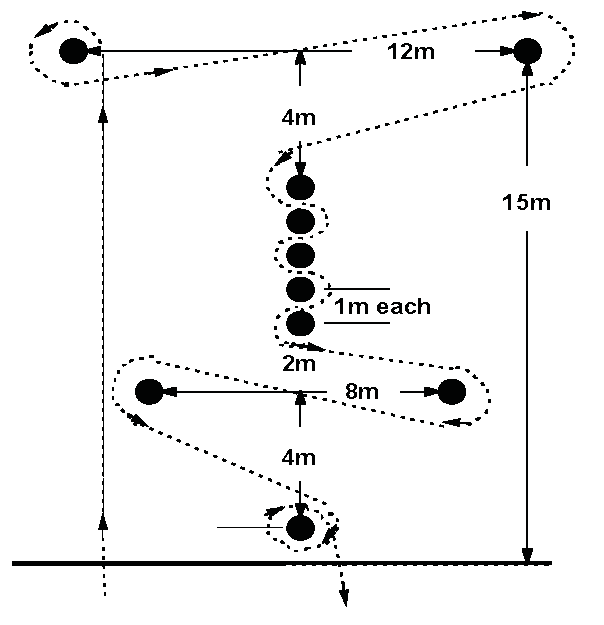
\includegraphics{iuf_slalom}
\end{center}
\vspace{-20pt}
\caption{IUF Slalom Course \label{fig:iuf_slalom}}
\vspace{-10pt}
\end{figure}
At right is the IUF Slalom, in which you must ride around 10 cones in the correct pattern.
Arrows marked on the ground should indicate the direction of the turns for riders unfamiliar with the course.
The rider has to start directly behind the Start line (as in other Track races).
The Starter gives the opening, and then the competitor has to start during the next 3 seconds.
The timer is started when the front of the wheel crosses above the Start line.
Cones may be hit, but not knocked over.
The course must be followed correctly, including the direction of turns.
The last cone must be completely circled before the rider's time is taken at the finish line.
Riders who go the wrong way around a cone can go back and make the turn the correct way with the clock still running.
The cones used are plastic traffic cones.
For official competition, cones must be between 45 and 60cm tall, with bases no more than 30cm square.
The course must be set up accurately.
The proper positions of the cones should be marked on the ground for a cone to be replaced quickly after it has been knocked over.
Riders get two attempts.

\section{Jumping Events \label{sec:racing_jumping-events}}
Unicycling versions of the High Jump and Long Jump 
\subsection{High Jump}
The rider and unicycle jump over a bar, without knocking it down, and ride away without a dismount.
There are three parts to a successful jump: 
\begin{enumerate}
\item Riders must mount before the start line, to show they are on the unicycle and in control.
The attempt starts when the rider crosses the start line.
The rider may break off from a jumping attempt before leaving the ground, but must then start again from behind the start line.
That attempt then doesn't count.
\item Riders must jump over the bar without knocking the bar off the apparatus.
The bar can be hit as long as it does not fall.
If the bar falls before the rider crosses the finish line, it counts as an unsuccessful attempt.
\item After landing, the rider must stay in control of the unicycle until he cross the finish line without dismounting, touching a hand to the ground or any other object, or knocking down the bar or any of the high jump apparatus.
Riders get two attempts at each height.
The rider starts at a low height and after each successful attempt, the height increases at set intervals until the rider fails to be successful on both attempts.
When the rider fails both attempts, the maximum height that was completed is recorded.
\end{enumerate}

\subsubsection{Unicycles}
Standard unicycles must be used (see definition).
No restriction on wheel or crank size.
For best results, metal pedals should be allowed for their strength and better grip.
This may make it impossible to hold this event on a sensitive track surface.
\textbf{Note:} In addition to the required safety gear for racing, helmets are required.

\subsubsection{Setup}
Around the High Jump apparatus a circle with a radius of 3 meters must be marked.
This circle is start and finish line.
The rider can cross it wherever he wants.
Riders must ride or hop across the finish line for the attempt to count.
Successfully crossing the finish line is judged the same as in racing (see section \ref{sec:racing_finishes}).
The bar must be held loosely in the jumping apparatus so it can fall or break away if the rider does not complete the desired height.
Magnetic systems are not allowed.
The bar shall have a minimum diameter of 2cm.

\subsubsection{Broken Unicycle}
If the unicycle breaks during an attempt, a new attempt must be given to the rider.

\subsection{Long Jump}
The rider jumps as far as possible from a jump marker, to a landing without a dismount.
The rider must then continue riding across a finish line to show control.
Riders must clear 3 markers (jump marker, landing marker and finish line) to make the jump count.
Riders may jump with the wheel going forward or sideways.
After landing, the rider must stay in control of the unicycle for the remainder of a 5-meter distance from the jump marker without dismounting, or touching a hand to the ground or any other object.
If the tire touches the jump marker before takeoff or the landing marker, it counts as a foul.
Riders may break off in a run as long as he is between start line and jump marker but if they cross or touch the jump marker, the attempt counts, including fouls.
Riders get two attempts for each length.
The farthest non-fouling, successful jump is recorded.

To avoid endless competitions, the length to jump will always increase by 5cm for each round.
Once there are only 5 riders left, it's up to the riders to decide in which steps they continue.
For each age group the minimum length should be adjusted to a useful level such as 150cm for 15+ and 70cm for 0-15.
The host can adjust this depending on the level at his competition.

\subsubsection{Unicycles}
Same as for High Jump.
\textbf{Note:} In addition to the required safety gear for racing, helmets are required.

\subsubsection{Setup}
The riding area consists of a start line, a jump marker, a landing marker and a finish line 6 meters beyond the jump marker.
Riders must ride or hop across the finish line for the attempt to count.
Successfully crossing the finish line is judged the same as in racing (see section \ref{sec:racing_finishes}).
The start line must be in the minimum 15 meters in front of the jump marker to be able to accelerate; behind the finish line must be an area which is 7 meter long and 2 meter wide in the minimum as safety zone.
Riders may use all or part of the 15 meters between start line and jump marker.
They are also allowed to start from beside to be able to do accelerated side jumps.
Markers for takeoff and landing (jump marker and landing marker) should be similar in shape to a meter stick, and be at least one meter in width (across the runway), no more than 5mm in height (above the runway), and no less than 3 centimeters in depth (front to back).
A Long Jump competition needs a minimum area of 28x2 meters.

\subsubsection{Judging}
The rider must clear the jump marker and the landing marker without touching them; he also has to clear the finish line to make it a valid jump.
Jump distance is measured between the outer edges of the jump and landing marker.
There has to be at least one judge (better two) to look at the markers.
For national championships and Unicons, two judges are always needed; one to observe each marker.

\subsubsection{Broken Unicycle}
If the unicycle breaks during the jump or landing, the rider will be given a new attempt.

\section{Alternate, Optional or Fun Events \label{sec:racing_alternate-optional-fun-events}}
These are optional events, not guaranteed to be included in every unicycle convention.
They can be held with as much, or as little, level of formality and importance the host chooses.
Age group breakdown is also up to the host.
All of the events in this section have been run before, using these rules.
If a large convention advertises events with the names of the ones detailed in this section, they must use the rules provided here.
If hosts desire to do variations on these rules, the events must be labeled accordingly.
Example: ``Track Gliding; Modified''.
In cases such as this, hosts must remember to provide detailed rules for these events at the same time the events are announced.

\subsection{4 x 100m Relay}
Usually 100m x 4.
The same rules as for track races apply.
Mixed male/female teams may be used.
Riders may remount if necessary, and must pick up the baton if it is dropped.
Usually there are no age groups.
If the baton is not handed over within the marked areas, the team will be disqualified.

\subsection{Coasting Events}
An event to determine which rider coasts the furthest distance.
Riders' coasting distances are measured from a ‘starting line' with a 5 meter minimum, which will be marked by a `qualifying line.'
If the rider does not cross the qualifying line it will count as a failed attempt.
The farthest distance from the line wins.
The distance is measured to the rearmost part of the rider that touches the ground when dismounting, or to the rear of the tire where the rider stops coasting.
Remounting is not allowed.
Riders must not touch any part of their tires, wheels or pedals while coasting.
Riders get two attempts.
If a rider crosses the coasting line (front of the tire) not in coasting position, he or she is disqualified in that attempt.
The riding surface should be as smooth and clean as possible, and it may be straight or curved.
Ample time must be allowed for all competitors to make some practice runs on the course before the official start.
The type of event(s) to be used should be announced well in advance of the competition.
Crank arm rules do not apply in any coasting or gliding events.

\subsubsection{Road Coasting}
This event is best held on a roadway with a very slight downward slope.
Riders are allowed an unlimited distance to speed up and start coasting before the starting line.

\subsubsection{Track Coasting \label{subsubsec:racing_alternate-optional-fun-events_coasting_track-coasting}}
30 meter starting distance.
This event is held only on a track, or a very level, smooth surface.
Wind must be at a minimum for records to be set and broken.
This event can be compared with other races at different tracks worldwide.

\subsubsection{Downhill Coasting}
This is a speed coasting event, with the same rules as section 
\subsubsection{``Downhill Glide,'' except riders must be coasting}
instead of gliding.
Dismounts before the finish line disqualify the rider in that attempt.
The slope must be very gradual for this event to be safe, and helmets are mandatory.

\subsubsection{Indoor Coasting}
30 meter starting distance.
This event is held indoors in a gym, or on a very level, smooth surface.
Rider will coast in a circle on the outer edge of the gym, separated by cones.
Both directions are allowed for the start (clockwise or counterclockwise), and rider will have a maximum of 30m before beginning to coast.
Indoor coasting is the recommended coasting competition at a Unicon.

\subsection{Gliding Events}
Gliding is like coasting, but with one or both feet dragging on top of the tire to provide balance from the braking action.
These events are similar to the coasting events above, with riders gliding for time or distance from a given point.
The rules are the same as for the coasting events (above) with the addition that the riding surface must be dry.
Coasting is allowed.

\subsubsection{Slope Glide Or Track Glide}
A slope glide can be done on a small hill.
Riders start on the hill, gliding down to level ground and continuing as far as they can before stopping.
This event can have a limited starting distance, or no starting distance at all, with riders gliding from a dead stop.
If it is a Track Glide, it is held on a track with the same rules as Track Coasting (see section \ref{subsubsec:racing_alternate-optional-fun-events_coasting_track-coasting}).

\subsubsection{Downhill Glide}
A downhill race for speed.
Riders start from a standstill, or speed up to the ‘starting line.' Riders are timed over a measured distance to the finish line.
Dismounts before the finish line disqualify the rider in that attempt.
Helmets are mandatory.

\subsection{Slow Forward}
The object is to ride in a continuously forward motion as slowly as possible without stopping, going backward, hopping, or twisting more than 45 degrees to either side.
Two different board sizes are used: Age 0-10: 10m x 30cm.
Age 11-UP: 10m x 15cm.
The Slow Race is measured using the bottom of the unicycle wheel.
Riders start with the bottom of the wheel on the starting line.
On command by the Starter, the rider must immediately start forward motion and let go of starting posts.
The timer stops the watch when the bottom of the tire touches either the finish line, or the ground after the line on boards that end at the finish line.
Riders can be disqualified for very slight stops or backward motions, twisting more than 45º to the side, riding off the sides of the board, or dismounting.
Riders get two attempts.
There are no crank arm length or wheel size restrictions for this event.
No safety gear is required.

\subsection{Slow Backward}
This is the same as the slow forward race \textit{except}: 0-10 ride on 60cm board, 11-Up ride on 30cm board.

\subsection{700c Racing}
Races of any length and type can also be conducted in a 700c wheel category.
\begin{itemize}
\item Maximum wheel diameter: 75cm.
\item If these races are intended to exclude 24$"$ wheels, sizes must be greater than 618mm.
\item No restrictions on crank length.
\item Beyond these, 700c unicycles must comply with all other requirements for racing unicycles.
\item The host may choose age groups.
\end{itemize}

\subsection{Unlimited Track Racing}
An unlimited race is one in which there are no unicycle size restrictions.
Any size wheels, any length crank arms, giraffes or any types of unicycles (see definition) are allowed.
All other Track racing rules apply.
Helmets are mandatory.

\subsection{Juggling Unicycle Race}
The traditional distance is 50m.
Riders use the 5m line from the One-Foot Race, and must be juggling when they cross this line.
Three or more non-bouncing objects must be used.
If an object is dropped (hits the ground) or the juggling pattern is otherwise stopped, the rider is disqualified.
Two balls stopping in one hand during a 3-ball cascade is defined as stopping.
Riders who start by juggling four or more objects may drop one, as long as their pattern continues, unbroken, into three.
The juggling pattern must be ‘in control' when the rider crosses the finish line.
‘Control' is determined by the Referee.

\subsection{Ultimate Wheel Race}
An ultimate wheel is a unicycle with no frame or seat.
The traditional distance is 10m for 0-10 riders, and 30m for 11-UP riders.
Maximum wheel size is 618mm (24$"$) for all ages, with 125mm minimum crank arm length or 250mm between pedal holes.
The host may allow other limitations, or none, if these details are announced well in advance.

\subsection{50m Fast Backward}
Riders must face and pedal backward.
The Starter lines up the rear of the tire above the start line.
Helmets are mandatory.
Timing is stopped when the rear of the tire crosses the finish line.

\subsection{Medley}
This is a race involving riding several different ways of riding.

\textbf{Example:} Forward 25m, seat in front 25m, one foot 25m, hopping 10m, with 5m transition areas.
Rules are set by the host.
Remounting is allowed.

\subsection{Slow Giraffe Race}
This is the same as slow forward, but on giraffes.
Helping hands can be used as starting posts.
No limits on size or gear ratio, but unicycles must have their pedal axle above the wheel axle, with a chain, belt, or other form of drive system.

\subsection{Road Races}
These are races held usually on roadways or bike paths, generally for longer distances than our events on the track.
All riders may race together and be separated by age group afterward.
If large numbers of riders will be on a narrow course, they must be started in smaller groups to facilitate passing and safety.
Water/food stations are recommended for events expected to last 30 minutes or more.
Helmets are required for all Unlimited riders, and for any Standard wheels larger than 29$"$ (768mm).
Personal music systems are not allowed for any races on public roads where there may be motorized traffic.
Non-lane passing rules apply (section \ref{subsec:racing_lane-use_non-lane-races}), but drafting is allowed.
Riders can be divided by age and/or unicycle type, such as 24$"$ and 29$"$ track unicycles, Standard (any size wheel and cranks), and Unlimited (see definitions).
24$"$ and smaller wheels are not recommended for very long races.
Traditional road race distances have been 10k and Full Marathon (42.195k).
Any distances can be used, but if specific distances are advertised, the race course must be measured to be the correct distance.

\section{Mountain Unicycling (MUni) \label{sec:racing_muni}}
For purposes of these rules, MUni refers to off-road races over any type of terrain.
Races can vary from a single heat race with all riders starting together, to a time-trial type of arrangement with riders going singly, at intervals.
Mountains are not required.
Terrain can be anything from dirt to paved areas, hills, ditches, curbs, rocks, sand, mud, or grass.
Unless otherwise noted, there are no restrictions on wheel size, crank arm length, brakes or gearing.

\subsection{Required Dress}
For all MUni events, riders must wear shoes, kneepads, gloves/wristguards and helmets (definitions, section 1.26). %TODO: ref needed
The IUF allows no exceptions to this for MUni events.
Additional equipment such as shin, elbow or ankle protection are optional.

\subsection{MUni Race Courses}
Courses must be clearly marked, so the first riders can easily see where to go.
Unless otherwise noted, non-lane passing rules apply (see section \ref{subsec:racing_lane-use_non-lane-races}).
A great MUni racecourse is often not the same as a great MUni trail, as there must be room to pass.
Though there can be narrow sections, a race course must allow enough room for riders to change positions in proportion to the amount of riders per heat.
For a mass-start race, there must be a wide enough starting area, and sufficient length at the beginning for riders to sort themselves by speed before the course narrows down.
A doubletrack, for instance, does not allow passing if there are too many riders in the same place.
A section of road or wide uphill area can provide space, as well as time to let riders spread out.
Mass-start events require multiple wide areas to allow passing.
All courses should strive for a balance of speed, excitement, and safety.
When course building, it is important to imagine what it would be like for ten or more people to fight over it at top speed.
Avoid trails that will not work for this, or plan for additional heats with smaller numbers of riders.
Look for areas that will create bottlenecks, such as technical spots and uphill areas, and plan the course so these areas do not have too many riders at the same time.

\subsection{Dismounts And Dismounted Riders}
Dismounts are allowed in all MUni races unless otherwise noted.
In mass-start events, dismounted riders must yield to mounted riders behind them as quickly as possible after a dismount, and until re-mounted.
Riders may not impede the progress of mounted riders when trying to mount.
If necessary they must move to a different location so mounted riders can pass.
If riders choose not to ride difficult sections of the course, they must not pass any mounted riders while walking or running through them.
In time trial-type events, see below for variations based on the other event details.
Violations of these non-riding rules may result in disqualification or a time penalty, to be determined and announced before the race start.
Riders must also ride completely across the finish line, as described in section \ref{sec:racing_finishes}.

\subsection{Uphill Race}
An Uphill MUni race challenges riders' ability to climb.
Courses may be short and steep or longer, endurance-related challenges.
Generally it is a timed event, but on an extremely difficult course, riders can be measured as to how far they ride before dismounting.
The race can be offered as a no-dismounts challenge, which either measures who gets the farthest, or disqualifies anyone who doesn't complete the distance without a dismount.
Multiple tries can be allowed, or the race can be a simple timed event.

\subsubsection{Dismounted Riders, Uphill}
If the Uphill race is run as a time trial, riders are intended to ride the entire distance.
In the event of a dismount, the rider must remount the unicycle:
\begin{itemize}
\item At the point where the dismount occurred if the unicycle falls back down the course toward the start.
\item Where the unicycle and/or rider come to a stop after dismounting.
Excessive running/walking/stumbling after a dismount may be grounds for a penalty at the discretion of race of the Referee.
\item Riders may also choose to back up (toward the start line) from one of those spots to remount, if they prefer the terrain there.
\end{itemize}

\subsection{Downhill Race}
A Downhill MUni race is a test of speed and ability to handle terrain.
Courses must be primarily downhill but may include flat or uphill sections.
Recommended course length is 2.5km, or 1km at a minimum, depending on available terrain, trails and schedule time.
Riders should race one at a time, released at regular time intervals.
If the schedule has a small time window for the race, riders should be run in heat sizes that allow passing on the course, and do not bottleneck at the beginning.

\subsubsection{Dismounted Riders, Downhill}
Dismounted riders must not impede the progress of, or pass mounted riders.
They must remain aware of riders coming from behind, and not block them with their unicycles or bodies.
Running is not allowed, except momentarily to slow down after a dismount.
Riders may walk if necessary.
Riders may receive a time penalty or be disqualified if they disregard this rule.

\subsection{Cross Country (XC)}
A Cross Country race should be at least 5km or longer, depending on available terrain, trails and schedule time.
It is basically any MUni race that is not specifically focused on downhill or uphill.
The course can contain any amount of uphill or downhill riding and is to be about fitness, and ability to ride fast on rough terrain.

\subsubsection{Dismounted Riders, XC}
If the event is held as a time trial, dismounted rider restrictions must be announced before the start of the race.
Depending on course length and difficulty, dismounted riders may be required to walk, or walk only limited distance, or have no restrictions at all.

\chapter{Freestyle and Standard Skills \label{chap:freestyle}}

\section{The Difference Between These Events}
In Standard Skill, riders demonstrate pure skill and mastery on a standard unicycle, by performing up to 18 skills they have pre-selected.
Standard Skill judging is based on the point value of the skills and quality of their execution, not the ‘show.’ In Freestyle, riders perform to music, with costumes, props and any kinds of unicycles.
Riders are judged not only on skill, but also on how well they entertain and put on a show.
There are Individual, Pair, and Group Freestyle events.

\section{Age Groups}
\textbf{Note:} Age groups may be different for different types of event.
The minimum allowable age groups are listed for each event.
Convention hosts are free to add more age groups.
Age group is determined by the rider’s age on the first day of the convention.
Junior Expert is open to all riders 0-14.
Expert is open to riders of any age, including 0-14.
Riders must state the age group in which they are entering for each artistic event in which they participate.

\textbf{Example:} Riders who enter Individual Freestyle as Experts can enter Pairs in their age group if they wish.
Riders are divided male/female in Standard Skill and Individual Freestyle, but not in Pairs or Group.

\subsection{Riders Must Be Ready}
Riders who are not ready at their scheduled performance time may or may not be allowed to perform after the last competitor in their age group.
The Chief Judge will remember to consider language barriers, and that riders may be engaged in convention work to slow them down.
Except for Standard Skill, a rider may not perform before a different set of judges than those that judged the rest of their age group.

\section{Performance Set-Up}
Competitors are allowed a maximum of two minutes to set up their unicycles and props in the performing area.
Competitors who take too long risk being disqualified.
An extension of the set-up time can be given only by the Chief Judge and must be requested in advance.
Competitors must show a legitimate need when requesting more time, such as numerous props or complicated special effects.

\section{Interruption Of Judging}
An interruption of judging can result from material damage, injury or sudden illness of a competitor, or interference with a competitor by a person or object.
If this happens, the Chief Judge determines the amount of time left and whether any damage may be the fault of the competitor.
Re-admittance into competition must happen within the regulatory competition time.
If a routine is continued and the competitor was not at fault for the interruption, all devaluations coming forth from the interruption will be withdrawn.

\section{Music \label{sec:freestyle_music}}
In Freestyle events, music is included in the judging and competitors should use it.
In Standard Skill music is not judged.
But background music will be provided during all Standard Skill routines, or competitors may provide their own.
Competitors may also, at their request, have no music played.
It is recommended to have one or more backup copies of all music in case of loss or damage.
For recordable disks, competitors are also recommended to test their music on multiple players to make sure it will work at competition time.

\subsection{Media Types}
The host is required to have the capability of playing recordable CDs.
Other media types may also be supported, at the host's discretion.
The Artistic Director is responsible for announcing what media types will be supported, and making sure the necessary equipment is provided.

\subsection{Music Preparation}
Competitors must provide their music in a type that is supported, and has been announced by the Artistic Director.
All music must be clearly labeled with the competitor name(s), age group, event type (such as Pairs), and if needed, the track number.
Whenever possible, competition music should be the first track on the CD.
The DJ (music operator) is not responsible for any errors resulting from unsupported types or mislabeled tracks.

\subsection{Music Volume}
Volume level is controlled by the DJ, at instructions from the Chief Judge.
The base volume for Freestyle music should be loud enough to sound clear, and be heard by all.
For Standard Skill, volume level should not be loud enough to interfere with judge communication, but otherwise similar to the level for Freestyle.
Some competitors' music may start with especially loud or quiet sections, and the DJ should be advised of these so volume levels do not get compensated in the wrong direction.
Some competitors may request that their music be played at lower levels.
These requests can be made directly to the DJ.
Requests for higher volumes must be approved by the Chief Judge, who has the option of passing this responsibility to the DJ.

\subsection{Special Music Instructions}
Some competitors may have special music instructions, such as stopping or starting the music at a visual cue, changing volume level during the performance, etc.
The DJ is not responsible for errors carrying out these instructions.
For best results, the competitor should supply a person to coach the DJ during the performance, so there are no mistakes.
If the DJ receives instructions that sound unusual, the Chief Judge should be consulted for approval.

\section{Announcing Of Results}
Final results will be continuously announced and/or posted for public view.
Results Sheets will be posted after each age category of an event.
The protest period begins at this point.

\section{Protests}
Must be filed in writing, within 15 minutes from the posting of event results.
Protest against judges’ scores is not permissible.
Protest is only possible against calculation mistakes or other mistakes not connected to the scoring.
The Chief Judge must resolve all protests within 30 minutes from receipt of the written form.

\section{Freestyle, Flatland, and Street Comp Judging Panel \label{sec:freestyle_judging-panel}}
There are three (or more) judges each of Technical and Presentation for Age Group competitions; five (or more) judges each of Technical and Presentation for Jr. Expert and Expert competitions (including Group).
All judges must attend a workshop provided as part of the convention schedule before the start of the Freestyle competitions.
Exceptions to workshop attendance are granted by the Chief Judge if judging rules have not changed since the previous judging experience and the judge has high Accuracy Scores.
Unless otherwise noted, judges at a Unicon must either speak English or have translation assistance for the specified language while judging.
Judges at other unicycle conventions should speak the dominant language of that convention or have translation assistance.

Judges' names must be provided to the Chief Judge (via email, FAX, or postal mail) by at least one month prior to the start of the unicycle convention and include the number of freestyle conventions where they have been a competitor, judge, or simply in the audience.
See section \ref{subsec:freestyle_judging-panel_group-freestyle-judges} and \ref{subsec:freestyle_judging-panel_individual-pairs-freestyle-judges} for description of which teams/countries are required to provide judges.
Judges must be at least 15 years of age at the start of the event.
Judges are recommended to be a current freestyle competitor, a former freestyle competitor, an active coach of freestyle routines, a proven judge at prior competitions, or an avid spectator who has observed many freestyle routines.
Details about the Standard Skill judging panel are covered in section \ref{sec:freestyle_std-judging-panel}.

\subsection{Selecting Judges \label{subsec:freestyle_judging-panel_selecting-judges}}
A person should not judge an event if he or she is:
\begin{itemize}
\item A parent, child or sibling of a rider competing in the event.
\item An individual or team coach, manager, trainer, colleague who is member of the same club specified in the registration form, colleague’s family etc.
of a rider competing in the event.
\item More than one judge from the same family judging the same event at the same time.
\end{itemize}
If the judging pool is too limited by the above criteria, restrictions can be eliminated starting from the bottom of the list and working upward as necessary only until enough judges are available.
If there are some candidates who have the same level of restrictions and judging score, their agreement about publishing the results need to be considered.
The eliminations must be agreed upon by the Chief Judge and Artistic Director, or next-highest ranking artistic official if the Chief Judge and Artistic Director are the same person.

\subsection{Assignment Of Age Group Judges}
Judges will be chosen from the list of judges as provided in section \ref{subsec:freestyle_judging-panel_individual-pairs-freestyle-judges}.
Judges who are competing in the event just before or just after the current category are eliminated from the list.
Judges will also be eliminated from the list for the current category as described in section \ref{subsec:freestyle_judging-panel_rating-judge-performance}.
The final selection of judges will be chosen based on their accuracy scores from the remaining list.
If chosen from a large pool of judges, categories with six or fewer entries will have a minimum of three Technical judges and three Presentation judges; categories with seven to twelve entries will have a minimum of four Technical judges and four Presentation judges; categories with over 12 entries will have at least five Technical judges and five Presentation judges.

\subsection{Assignment Of Expert (And Junior Expert) Judges \label{subsec:freestyle_judging-panel_assignment-of-expert-judges}}
Assignments for Expert and Jr. Expert judges will be made by the Chief Judge using the most qualified of all judges available.
Qualifications are determined in the following order of importance: 
\begin{itemize}
\item Highest judging accuracy scores obtained while judging age group (age groups judges must have a minimum of five entrants) or other Jr. Expert and Expert events.
\item Greatest amount of Jr. Expert and Expert judging experience.
\item Greatest amount of international judging experience.
\item Greatest number of Freestyle competition experienced (viewed, judged, or as a competitor).
\end{itemize}
Judges who are competing in the event just before or just after the current category are eliminated from the list.
Judges will also be eliminated from the list for the current category as described in section \ref{subsec:freestyle_judging-panel_selecting-judges}.
Judges will also be eliminated from the list if they exhibit Judging weaknesses during their Age Group judging as described in Section \ref{subsec:freestyle_judging-panel_rating-judge-performance}.
At Unicons, if more than five judges each of Technical and Presentation remain, judges who have not judged at a previous Unicon will be removed from the list.
If there are still more than five each then the final list of judges for the category will be chosen by accuracy scores as defined in section \ref{subsec:freestyle_judging-panel_calculating-accuracy-scores}.

\subsection{Standard Skill Vs. Freestyle Vs. Flatland or Street Comp Judging}
With entirely different sets of rules, qualified judges for Standard Skill are not necessarily qualified to judge Freestyle, the Street Comp, Flatland, and vice versa.
Judges' qualifications must list the types of events they are qualified to judge.

\subsection{Judging Panel May Not Change}
The individual members of the judging panel must remain the same for entire age groups; i.e. one judge may not be replaced by another except between age groups.
In the event of a medical or other emergency, this rule can be waived by the Chief Judge.

\subsection{Rating Judge Performance  \label{subsec:freestyle_judging-panel_rating-judge-performance}}
Judges are rated by comparing their scores to those of other judges at previous competitions.
Characteristics of Judging Weaknesses
\begin{itemize}
\item \textbf{Excessive Ties:} A judge should be able to differentiate between competitors.
Though tying is most definitely acceptable, excessive use of tying defeats the purpose of judging.
\item \textbf{Group Bias:} If a judge places members of a certain group or nation significantly different from the other judges.
This includes a judge placing members significantly higher or significantly lower (a judge may be harsher on his or her own group members) than the other judges.
\item \textbf{Inconsistent Placing:} If a judge places a large number of riders significantly different from the average of the other judges.
\end{itemize}

\subsection{Re-Instating Judges}
If a judge has been labeled as having a Judging Weakness, they may have a chance to be re-instated on the list by:
\begin{itemize} 
\item Discuss with the Chief Judge the scores that were Tied, Biased, or Inconsistent.
\item Practice judge on at least two categories with at least 4 competitors.
\end{itemize}
If the practice judging shows no further examples of Judging Weakness, they may be reinstated on approval by the Chief Judge and Artistic Director.
If the Chief Judge and Artistic Director are the same person, then the next highest-ranking official must agree to the reinstatement.

\subsection{Calculating Accuracy Scores \label{subsec:freestyle_judging-panel_calculating-accuracy-scores}}
The score for each judge will be calculated using a pre-defined calculation that is shared with all judges and other interested people.
The calculation takes into account all types of mistakes and sums each mistake.
A judging score of 0 would be perfect; anything between 10 and 15 shows signs of Judging Weakness; scores of over 15 indicate a Judge with Weaknesses who should be removed from the list of available judges.

\subsection{Group Freestyle Judges \label{subsec:freestyle_judging-panel_group-freestyle-judges}}
Countries must provide a minimum of one judge (either Technical or Presentation) for each group entered in Group Freestyle.
Each country is allowed to provide two more judges than the number of groups competing in the event.
For example: Country-A has three groups competing in Group Freestyle.
Country-A is required to provide at least three judges (one from each group), but no more than five judges.
If a country is having difficulty finding qualified judges, they may ask a known judge from another country to represent them.
Countries without a competing group may also enter a maximum of two judges.
The names of the judges will be provided by either the team leaders of each group and/or primary contact for that country.
If too many names are provided by the team leaders and/or primary contact for the country, the country's judges will be chosen based on the criteria outlined in section \ref{subsec:freestyle_judging-panel_assignment-of-expert-judges}.
Judges who have shown a tendency to be a Judge with Weaknesses (defined in section \ref{subsec:freestyle_judging-panel_rating-judge-performance}) will have their name removed from the pool of available judges.
If more than ten judges are provided, the final judging panel of ten will be selected by their accuracy scores as defined in section \ref{subsec:freestyle_judging-panel_calculating-accuracy-scores}.

\subsection{Individual And Pairs Freestyle Judges\label{subsec:freestyle_judging-panel_individual-pairs-freestyle-judges}}
Countries must provide a minimum of one judge for every five entries they have for Individual and Pairs Freestyle.
Number of entries will be rounded up to the next nearest multiple of 5.
For example: If a country has 1 entry, they must supply at least one judge.
If a country has 11 entries, they must supply at least three judges.
If a country is having difficulty finding qualified judges, they may ask a known judge from another country to represent them.
Countries may also apply to the Chief Judge for help in finding judges from outside their country to represent them.
Countries with no entries in Individual or Pairs Freestyle may also enter a maximum of two judges.
The names of the judges will be provided by either the team leaders from the Individual and Pairs competitors and/or primary contact for that country.
Countries not required to supply more than a maximum of ten judges for the Individual and Pairs Freestyle competition.
If a country submits more than ten judges, after elimination of known Judges with Weaknesses (defined in section \ref{subsec:freestyle_judging-panel_rating-judge-performance}), the judges for that country will be chosen based on their accuracy scores.

\subsection{Not Providing Judges}
At Unicons, countries that are unable to provide their required number of judges (either Group or Individual/Pairs) may have their competitors removed from that competition.
Exceptions will be granted on a special basis with a letter to the Chief Judge, Artistic Director, and Unicon Director.

\subsection{Judges Workshop}
The hosts of the convention must provide for a judge’s workshop at least 24 hours prior to the start of the Freestyle competition.
A minimum of 3 hours must be set aside, in a classroom or similar environment.
If possible, it is strongly recommended to have more than one workshop to accommodate schedules.
Variations on this can be approved by the Chief Judge.
Workshop schedule(s) must be announced to all judges at least three weeks prior to the start of the competition.

Judges should have read the rules prior to the start of the workshop.
The workshop will include a practice judging session.
Each judge will be required to sign a statement indicating they have read the rules, attended the workshop, agree to follow the rules, and will accept being removed from the list of available judges if their judging accuracy scores show Judging Weaknesses.

\section{Scoring}
In all events except Standard Skill, the scores of each judge are transferred into placing points, which represent the ranking of each competitor by that judge.
The highest scoring competitor gets 1 placing point, the next one gets 2, and so on.

\textbf{Note:} The ranking number, or highest placing point available for a competitor depends on the number of entries in that category.
If two or more competitors have the same score, they are awarded equal portions of the total number of placing points available for the places they occupy in the ranking.

\textbf{Example:} Seven competitors.
Four of them tie for 2nd place.
7th place gets 7 points, 6th place gets 6 points, and 1st place gets 1 point.
For the other four competitors, add up the other placing points numbers: $2+3+4+5=14$.
Divide this by the number of competitors (4) to get 3.5 placing points each.

\subsection{Removing The High And Low}
After determining placing points as above, discard the highest and lowest placing score for each rider.
If Rider A has scores of 1,2,1,3,2, take out one of the ones, and the three.
Then Rider A has 1,2,2, for a total of 5.
If Rider B has scores of 2,2,2,2,2, he will end up with 2,2,2, a total of 6.
The winner is the competitor with the lowest total placing points score after the high and low have been removed.

\subsection{Ties}
If more than one competitor has the same placing score after the above process, those riders will be ranked based on their placing scores for Technical.
The scoring process must be repeated using only the Technical scores for the tied riders to determine this rank.
High and low placing scores are again removed in the process.
If competitors' Technical ranking comes out equal, all competitors with the same score are awarded the same place.

\section{World Champions \label{sec:freestyle_world-champions}}
Winners in the Expert category of each event are the \textbf{World Champions}.
In the individual events, separate titles are awarded for male and female.
Winners in the Jr. Expert category are the \textbf{Junior World Champions}.

\newpage
% Freestyle Rules

\section{Individual Freestyle Overview}

\subsection{Minimum Age Groups}
 0-14, 15-UP, Expert.
The decision to enter as Expert or Jr. Expert is optional, but must be stated in advance.

\subsection{Time Limits}
2 minutes for riders 0-14 (except Jr. Expert), 3 minutes for all other age groups (except Expert).
Jr. Expert has a maximum of 3 minutes and Expert has a maximum of 4 minutes.

\subsection{Unicycles}
Any type and any number.

\subsection{Music, Costume and Props}
All are judged, and must be considered in the performance.
Check the rules of the specific convention for prop restrictions.
Fire and sharp objects (i.e. juggling knives) are prohibited.

\subsection{Judging Method}
Riders’ scores are divided into two parts called Technical and Presentation, each receiving 50\% of the score.
Read the Freestyle Judging section to learn more.

\subsection{Maximum Number of Competitors for Jr. Expert and Expert}
\textbf{Non-Unicon:} Organizers of non-Unicon events can choose to limit the number of competitors using the guidelines below or have no limit.
\textbf{Unicon:} Each country can submit a maximum of three individuals in each category to compete at Unicon in the Individual Freestyle events (three in Jr. Expert Male, three in Jr. Expert Female, three in Expert Male, three in Expert Female).
If a country has placed 1st, 2nd, or 3rd in Individual Freestyle at the previous Unicon, they can submit one additional competitor for each placing in that category.
For example, if Country-A wins first place in Expert Male at the previous Unicon, they may submit up to four individuals for Expert Male at the current Unicon.
If Country-B wins second and third place in Jr. Expert Female at the previous Unicon, they may submit up to five individuals in Jr. Expert Female at the current Unicon.

\subsection{Method for Limiting the Competitors at Unicon}
A country that wishes to submit more than their allocated number of individuals should select individuals by their own way.
Any type of competition using the IUF judging methods to determine their competitors is recommended.
If a country is unable to hold a competition, a country can choose individuals by their own rating method.
For example, if a country has placed 1st, 2nd or 3rd in Individual Freestyle at the previous Unicon, it can give these individuals a higher rating, because they brought additional number of individuals to a country.
If a country did not place in the top three, it can give only the highest placing individual a higher rating.
It is strongly recommended to complete the selection at least three months prior to the start of the Unicon.
If a country cannot select by then, the method and schedule of the selection must be communicated to the Chief Judge and Artistic Director at least three months prior to the start of the Unicon.

\section{Pairs Freestyle Overview}

\subsection{Minimum Age Groups}
Age group (all ages), Expert.
Each rider may enter only once.
The age group of the older rider is the age group for the pair.
Expert is treated as the ``oldest'' age group, followed by Jr. Expert, and then all other age groups.
The decision to enter as Expert or Jr. Expert (if used) is optional, but must be stated in advance.

\subsection{Time Limits}
Same as Individual Freestyle.

\subsection{Unicycles}
Any type and any number.

\subsection{Music, Costume and Props}
Same as Individual Freestyle.

\subsection{Judging Method}
Same as Individual Freestyle, 50\% for Technical, and 50\% for Presentation.
In Pairs, there is extra emphasis on teamwork; two person skills, etc.
(see Judging Criteria).

\subsection{Maximum Number of Competitors for Jr. Expert and Expert}
\textbf{Non-Unicon:} Organizers of non-Unicon events can choose to limit the number of competitors using the guidelines below or have no limit. 
\textbf{Unicon:}Each country can submit a maximum of three pairs in each category to compete at Unicon in the Pairs Freestyle events (three in Jr Expert Pairs, three in Expert Pairs).
If a country has placed 1st, 2nd, or 3rd in Pairs Freestyle at the previous Unicon, they can submit one additional competitor for each placing in that category.
For example, if Country-A wins first place in Expert Pairs at the previous Unicon, they may submit up to four Pairs for Expert Pairs at the current Unicon.
If Country-B wins second and third place in Jr Expert Pairs at the previous Unicon, they may submit up to five pairs in Jr Expert Pairs at the current Unicon.
If a pairs team is submitted consisting of members from two countries, that team must choose one of their two countries to represent.

\subsection{Method for Limiting the Competitors at Unicon}
A country that wishes to submit more than their allocated number of pairs should select competitors by their own way.
Any type of competition using the IUF judging methods to determine their competitors is recommended.
If a country is unable to hold a competition, a country can choose pairs by their own rating method.
For example, if a country has placed 1st, 2nd, or 3rd in Pairs Freestyle at the previous Unicon, it can give these pairs a higher rating if BOTH partners from the previous Unicon still be pairs, because they brought additional number of pairs to a country.
If a country did not place in the top three, it can give only the highest placing pairs a higher rating.
It is strongly recommended to complete the selection at least three months prior to the start of the Unicon.
If a country cannot select by then, the method and schedule of the selection must be communicated to the Chief Judge and Artistic Director at least three months prior to the start of the Unicon.

\section{Group Freestyle Overview}

\subsection{Minimum Age Groups}
None.

\subsection{Minimum Number of Riders}
Three.
Each rider may enter Group Freestyle only once.
A rider may appear in a second Group Freestyle performance with permission of the Chief Judge, to replace a rider due to illness, injury or other mishap.

\subsection{Time Limit}
Six minutes.

\subsection{Unicycles}
Any type and any number.

\subsection{Music, Costume and Props}
Same as Individual Freestyle.

\subsection{Juding Method}
Same as Individual Freestyle, but with additional emphasis on teamwork and multiple person skills, such as formation riding.
Extra consideration will be given to account for widely different group sizes, relative skill levels, and relative ages of riders.

\subsection{Maximum Number of Competitors for Jr. Expert and Expert}
\textbf{Non-Unicon:} Organizers of non-Unicon events can choose to limit the number of groups using the guidelines below or have no limit.
\textbf{Unicon:} Each country can submit a maximum of two groups to compete at Unicon in the Group Freestyle event.
If a country has placed 1st, 2nd, or 3rd in Group Freestyle at the previous Unicon, they can submit one additional group for each placing.
For example, if Country-A wins first place at the previous Unicon, they may submit up to three groups at the current Unicon.
If Country-B wins second and third place at the previous Unicon, they may submit up to four groups at the current Unicon.

\subsection{Method for Limiting the Competitors at Unicon}
A country that wishes to submit more than their allocated number of groups should select groups by their own way.
Any type of competition using the IUF judging methods to determine their groups is recommended.
If a country is unable to hold a competition, a country can choose groups by their own rating method.
For example, if a country has placed 1st, 2nd, or 3rd in Group Freestyle at the previous Unicon, it can give these groups a higher rating, because they brought additional number of groups to a country.
If a country did not place in the top three, it can give only the highest placing groups a higher rating.
Not all members from the previous Unicon are required to be members of a new group.
It is strongly recommended to complete the selection at least three months prior to the start of the Unicon.
If a country cannot select by then, the method and schedule of the selection must be communicated to the Chief Judge and Artistic Director at least three months prior to the start of the Unicon.

\section{Deadline For Signing Up}
These events have a deadline for entry, which must be specified in the registration form.
If not specified in the registration form, the deadline is one month before the official convention start date.
A maximum of ten Individuals, ten Pairs routines, and two groups will be allowed to be added after this time to account for difficulties in travel planning or other valid reasons that are communicated about in advance.
These will be added in the order of their request to the Chief Judge and Convention Director via email or fax.
Participants who attempt to sign up less than 36 hours prior to the beginning of the specified competition will not be allowed to enter.
Changing Pairs partners is allowed up to 36 hours prior to the actual competition as long as the category does not change.
Adding or subtracting the members of a group routine is allowed up to 36 hours prior to the start of that competition.

\section{Size Of Performing Areas}
Required spaces for the various events are listed below.
But riders, especially large groups, will want to know the overall amount of space that will be possible to ride on.
Hosts must publicize the dimensions of the available performing area as far in advance of the competition as possible, and organizers of international championships at least three months prior to the event.

\subsection{Individual And Pairs Performing Area}
For international competitions, the performing area must be no smaller than 14m wide x 11m deep.
At smaller events, smaller sizes can be used, but no smaller than 12m wide x 9m deep.
The boundaries of the performing areas must be clearly marked on the floor, with lines at least 3cm wide.
The distance between the outer edges of the performing areas and walls, poles or other stationary objects must be no less than 50cm.
Individuals or pairs who go outside the performing area may get a reduced score (see Judging Criteria).
Skills performed outside the Technical Judging Area (TJA), which is the same size as standard skill, will not affect the Technical score.
Presentation will be judged both inside and outside the TJA.
Going outside the TJA does not give a reduced score in Presentation.
The TJA is recommended to be placed in the middle of the performing area, and the layout of the TJA is also required to be publicized by the hosts as far in advance of the competition as possible.

\subsection{Group Freestyle Performing Area}
For international competitions, the performing area must be no smaller than 26m wide x 14m deep.
Groups who go outside the boundaries may get a reduced score, if the boundary is marked on the floor (see Judging Criteria).

\section{Order Of Performance}
Performance order for Jr. Expert and Expert in Pairs/Individual/Group freestyle are defined by an open drawing without a computer.
The drawing/selection should be done publicly and transparently, at a time that is pre-announced, so people can witness it.
The method to determine performance order for age groups is completely up to the Artistic Director.

\section{Start Of Performance}

\subsection{Freestyle Events}
The judging, the stopwatch, and the ‘performance’ all start at the same time.
The Timer starts the watch at the beginning of the music, or at a signal from competitors, whichever comes first.
The signal can be a nod, wave, bow, verbal cue (``Start!'') or any clearly understandable means.
An acoustic signal (such as a whistle) will indicate that the timing and judging have started.
Any non-unicycling activities such as dancing, posing, acrobatics, etc., must be included within the time limit of the routine to be judged.
In all Freestyle routines, an acoustic signal will indicate when there are 30 seconds left.
In all artistic events, two acoustic signals or a different signal will indicate the end of the riding time and end of the judging.

\section{End Of Performance}
The performance ends at a signal from the rider, such as a bow or ``Thank you,'' an obvious endpoint, or at the end of the time limit.
Nothing that occurs after the time limit may affect judging scores.

\subsection{Freestyle Events}
An acoustic signal will indicate the end of the time limit.
Any figures or performing that are done after the end of the time limit will not be judged Performing past the time limit will reduce the rider’s score.
All time limits are maximums.
Riders need not fill the entire time, but a routine that is very short may suffer in points over a routine with more content.
However, a routine that is boring, repetitive or ‘padded’ may lose points for being too long.
The rider must decide what makes the best performance.

\subsection{Performance Time Announcement}
When a Freestyle performance is finished, the timer will report the actual length of the performance.
The time can be either displayed visually or announced publicly.
A visual display must be visible to the judges and audience, such as on an electronic timing board or written on a whiteboard.
If the routine ran overtime, only the maximum time need be displayed (example: 4:00 for Experts), or nothing at all.
For public announcements by voice, the announcement should happen after the performer has exited, or clearly finished performing.
In other words it is preferred to wait if the performer has an artistic exit, even though it cannot be judged.
Then the announcement should be made, in a form similar to ``The performance time was two minutes, forty two seconds.'' This announcement must be made without delay, as it is a factor in the judging of the performer.
If the performance ran overtime, no voice announcement is needed.

\section{Rider’s No-Signal Option}

\subsection{Freestyle Events}
A rider may have a well-planned routine to music that he or she knows is under the time limit, and does not wish for the acoustic signals to detract from his or her performance.
When riders sign up with the Rider Liaison they can request ``No acoustic signals.'' This will eliminate the ‘Start’ signal, and the 30-second warning.
The Timer will still keep the time, and if the rider exceeds the time limit, the Timer will make the ‘double acoustic signal’ to indicate the rider has run overtime.

\section{Clean-Up}
In unicycling, a clean, dry riding surface is essential.
After a performance, the riding area must be left the way it was before the performance.
Riders and their helpers must clear all props, unicycles, and debris from the performing area within two minutes.
The next rider may also be setting up during this time.

\section{Messy Performing Area}
Riders who are thinking of using messy props in their performances must carefully consider the above rule.
Popping balloons, dirt or powder, confetti, water, pies, etc.
may take longer than two minutes to remove.
Special permission must be received from the Chief Judge or Artistic Director before any such props are used.
Competitors who make messes they are unable to remove may be disqualified from the event.

\newpage
%Freestyle Judging

Judging for Individual, Pairs, and Group Freestyle is divided into two components, Technical and Presentation.
Qualified judges may judge only Technical, only Presentation, or both.
For each component, judges give four scores from 0 to 10, or 0 to 15, high scores being better.
Scores such as 2.0, 2.2, or even 2.25 are encouraged to help differentiate between riders of similar ability.

The scores given should match the description of the Example Scoring.
For example, if there are only two competitors in a category where the first rider has 2 major dismounts and the second rider has over 20 major dismounts, a score of 10 should not be given for ``Dismounts'' for the first rider even though the dismounts were significantly fewer.
Judging for Flatland and the Street Comp is described in sections 4.11 and 4.13. %TODO: references
Each judge gives scores for the complete performance.

\section{Individual Freestyle - Technical Score \label{sec:freestyle_individual-technical-score}}
The Technical part of the judging is broken into four parts.
Four scores will be given by each judge, values ranging from 0 to 10, or from 0 to 15 as follows: 
\begin{itemize}
\item Quantity of Unicycling Skills And Transitions (0-10 points) 
\item Mastery And Quality of Execution (0-15 points) 
\item Difficulty And Duration (0-15 points) 
\item Interpretation: (0-10 points)
\end{itemize}
\textbf{Technical Total:} 50 points

Skills done outside the TJA (Technical Judging Area) are not counted for the Technical Judge.

\subsection{Quantity of Unicycling Skills and Transitions}
\textbf{Quantity} is the number of unicycling skills and transitions successfully executed.
Transitions, before and after the skill, should also be counted.
If a dismount happens during transition but after a skill was successfully executed, only the completed skill is counted and the failed transition should not be counted.
For example, if a dismount happens during standup gliding, only the transition from riding to standup is counted.
If a dismount happens after standup gliding and during the transition from the standup gliding to riding, the previous transition into stand up and the standup gliding are counted.

Only `unicycling skills' will be counted (see Section 1.26 for definitions).
For example, if a rider is juggling while idling, idling is counted as a unicycling skill and juggling will affect the Interpretation: Props and other Presentation scores.
Performing many short skills with quick transitions can increase this score, but will decrease the score as related to the Duration score.

\textbf{Variety:} Different from Variety in Standard skill, different variations of the same type of skill are counted separately.
Skills should be chosen to work with the style of the performance, but performing exactly the same skill multiple times will decrease this score.

Examples:
\begin{itemize}
\item `Drag seat in front' and `drag seat in back' are counted independently.
\item The following variations of `standup gliding one foot' will be counted differently;
	\begin{itemize}
 	\item Arabesque (The free leg is extended behind the body above hip height – at least a 90 degree angle)
	\item Knee hold (one hand supporting the knee of the free leg)
	\item Y-character balance (holding a straightened leg up with one hand and using other hand to form a Y shape)
	\item Catch-foot (the free leg being held in one or both hands)
	\item Biellmann (the free leg grasped from behind and pulled overhead in the Biellmann position) 
	\end{itemize}
\item Face up spins are different from normal upright spins 
\item Combinations of one-rotation spins/turns are different from continuous spins
\end{itemize}

\textbf{Originality:} In Freestyle, new skills are less important than in Flatland.
However, skills with unique variations that are completely new or with new approaches will get more points.
Originality is mainly judged in Presentation (section \ref{sec:freestyle_individual-presentation-score}).

\textbf{Scoring Guidelines for Quantity of Unicycling Skills and Transitions (Variety and Originality):}

\begin{tabular}{|l|p{12.5cm}|}
\hline
10 & Perfect - No room to add more skills with impressive originality \\
\hline
8 & Excellent - Filled with many skills with proper pause and variations and/or some originality \\
\hline
5 & Medium level - average number of skills and variations \\
\hline
2 & Lower number of skills without proper variations \\
\hline
0 & There are no unicycling skills \\
\hline
\end{tabular}

\subsection{Mastery And Quality of Execution}
\textbf{Mastery} is the amount of control shown by the rider(s) during their execution of the skills and transitions.
The body form should demonstrate good control and Mastery of the unicycle.
If a rider is showing good style (section \ref{subsec:freestyle_individual-presentation-score_choreography-style}) during difficult skills, the Mastery score should be high.
Mastery of the unicycling skills is also required to perform the ``additional non-unicycling skills'', such as juggling, dancing, and acrobatics.

There are several viewpoints to check the Quality of Execution, such as Stability, Duration, Speed, Synchronization, and Fluidity of Transition.
These viewpoints don't have to be evenly weighted, but required to check.

\textbf{Duration:} Holding a skill for a longer amount of time and distance also indicates a higher level of mastery and difficulty for that skill.

\textbf{Stability:} High scores should not be given if unintentional jerky body movement, or a wandering spin or pirouette is shown occasionally.

\textbf{Speed:} High score is given when the rider controls the speed (faster or slower) of turns, spins, and transitions excellently.

\textbf{Synchronization:} Being synchronized with the rhythm of the music and timing accuracy should be judged.
High scores are awarded for a routine if timing of the skills is well planned and accurate.

\textbf{Fluidity of Transition:} High scores are given for transitions when the rider performs a skill straight into another skill quickly.
Low scores are given for transitions if several revolutions, idles, hops (or other setup-type skill) need to be performed before performing the more difficult skill - unless it is obvious that these are used to increase the overall choreography and timing of the routine.

\textbf{Scoring Guidelines for Mastery and Quality of Execution (Stability, Duration, Speed, Synchronization, Fluidity of Transition):} 

\begin{tabular}{|l|p{12.5cm}|}
\hline
15 & Perfect - No room to improve; never loss of control; all criteria are perfect \\
\hline
13 & Almost perfect - Almost all criteria are perfect without loss of control \\
\hline
11 & High Level - Excellent Mastery and Quality but some loss of control \\
\hline
8 &  Medium level - All criteria are average level \\
\hline
4 & Low Level - All criteria are lower than average \\
\hline
1 & Beginners Level – None of the criteria are followed \\
\hline
\end{tabular}

\subsection{Difficulty And Duration}
The level of Difficulty is taken into account for successfully executed skills including transitions.
High scores are awarded for a routine packed with a number of skills all with high difficulty.
High scores should not be given if only one or two of the skills are of a high level.
Generally:
\begin{itemize} 
\item Backward skills are more difficult than the same type of Forward skills.
\item `Seat against body' is easier than `Seat not touching body'.
\item Faster spins/turns with smaller diameter are more difficult than slower spins/turns with larger diameter.
\item `Stand up with a hand touching the seat' is easier than `stand up with neither hand touching the seat'.
\item `Jump up from the pedals to the frame removing both feet simultaneously' is more difficult than `Standup with one or both feet on the frame'.
\end{itemize}
If a rider is juggling while idling, for example, the difficulty of idling does not carry the same difficulty as idling without juggling.
The same applies for dancing, and acrobatics.

\textbf{Duration:} Holding a skill for a longer amount of time and distance also indicates a higher level of mastery and difficulty for that skill.

\textbf{Scoring Guidelines for Difficulty and Duration:}

\begin{tabular}{|l|p{12.5cm}|}
\hline
15 & All very difficult skills with long duration \\
\hline
13 & Almost all skills are at high difficulty with enough duration \\
\hline
10 & Many skills at high difficulty but some skills with short durations \\
\hline
8 & Generally average or higher difficulty but some skills with short duration \\
\hline
6 & Generally lower than average or higher difficulty but many skills with short duration \\
\hline
4 & Only one or two skills at high level and/or many skills with short duration \\
\hline
2 & O.K. and skills done reasonably long without compromising flow of routine \\
\hline
0 & Looks like will fall constantly; much repetition of skills; low difficulty when averaged for whole routine. \\
\hline
\end{tabular}

\subsection{Technical Interpretation}
How skills, costume, music, props (if used), and style all work together to present a theme to the whole routine from a technical point of view.
If one part is removed, the whole performance would suffer.
The elements should be consistent and this section rates how well the whole routine is put together.

\textbf{Skills:} Should be chosen to work with the costume, music, and style to create an integrated theme.
If the routine is flowing and smooth with graceful body style, skills that are less graceful (typically seat out skills) should not be used.
The choice of skills is the most important part in Technical Interpretation.

\textbf{Costume:} A costume is chosen to enhance the routine.
If costume(s) are chosen that have the potential to impede riding but the competitor(s) successfully adapt the costume to add to the whole performance, they should be given extra points.

\textbf{Music:} Judges are looking for music that is selected to put whole routine together.
Skills are chosen carefully to match the feeling and tempo of the music.
Music that is simply background or not integral to the routine is considered a poor choice.
A high scoring routine is where the rider uses the sound, beat, theme, or changes in the music as integral parts of the routine.
If music is chosen that is too long for the allowed time, the competitor should be penalized here.

\textbf{Props:} A unicycle, when used for anything but a unicycling skill (handstand on the unicycle while it is lying down, hopping standing on the frame with wheel and seat on the floor) is considered a prop.
Other props can be removable parts of the costume (hats, clothing, etc), items placed to set a scene, a person.
Note that it says ``Use of.'' This score is not awarded for the props, but for the effect of such props on the performance.
The judges are looking not for the props themselves, but how they are used.
It is not mandatory to include props in the performance.
If none are used, the score will not be lower.

\textbf{Style:} The body form is used to express the whole mood or theme of the piece by positioning and movements of the body during the routine.
Routines that show deliberate body form during the whole routine, especially during more difficult skills, should score higher than one with style and poses only during stable riding positions.
Judges look for deliberate movements over uncoordinated movements made to retain balance.
For example, if a graceful balletic routine, style should be graceful and flowing; if a technical/street theme, then the style should match that theme.
Other non-unicycling skills such as dance, mime, comedy, juggling, acrobatics, playing music, etc., are considered with this score.
These skills should add to the theme of the routine.

\textbf{Scoring Guidelines for Technical Interpretation (Skill, Costume, Music, Props if used, Style):}

\begin{tabular}{|l|p{12.5cm}|}
\hline
\textbf{Score} & \textbf{Samples of observed riding}  \\
\hline
10 & Routine is complete - cutting out one part will ruin the whole performance.
Skills chosen to accentuate the overall performance. \\
\hline
8 & If props used, four of the five elements (skills, costume, music, props, style) working together to present a theme but one obviously missing or mismatched.
If props not used, only three of the four elements working together. \\
\hline
6 & If props used, only three of the five elements working together to present a theme but one obviously missing or mismatched.
If props not used, only two of the four elements working together. \\
\hline
2 & Part of routine looks integrated, but several elements are not working (music not matching, costume choice interferes, props clumsy, or skills don't match the music). \\
\hline
0 & Routine looks thrown together, with no thought of whole performance. \\
\hline
\end{tabular}

\section{Individual Freestyle – Presentation Score \label{sec:freestyle_individual-presentation-score}}
The Presentation part of the judging will be broken into four parts.
Four scores will be given by each judge, values ranging from 0 to 10 or from 0 to 15 as follows:
\begin{itemize}
\item Mistakes: Dismounts and Boundary (0-10 points) 
\item Choreography And Style (0-15 points) 
\item Showmanship And Originality (0-15 points) 
\item Interpretation: (0-10 points)
\end{itemize}
\textbf{Presentation Total: 50 points}

Presentation will be judged both inside and outside the TJA (Technical Judging Area).

\subsection{Mistakes: Dismounts and Boundary}
Low scores are given for routines with more than 8 major dismounts, therefore interrupting the flow of the routine.
Medium scores are given for a routine that has approximately 3 major dismounts and a few minor dismounts.
High scores are given for a routine with no major dismounts, and few or no minor dismounts.
Judges need to be able to differentiate between a planned dismount and an unplanned dismount.

\textbf{Major} dismounts are when the unicycle falls and/or a hand or any body part other than the rider's foot or feet touch the floor.
Major dismounts are also when the choreography of a rider's routine is clearly affected.

\textbf{Minor} dismounts are when the unicycle does not fall, only the rider's foot or feet touch down and the choreography of a rider's routine is not affected.
A minor dismount may also be counted when Judges cannot differentiate between a planned dismount and an unplanned dismount.

\textbf{Boundary:} There is a Technical Judging Area (TJA), which is 14m wide x 11m deep, and a Performing Area, which may be larger than the TJA if the facilities permit a larger area.
Both boundaries are marked.
Skills performed outside the TJA are not judged.
Boundary issues are applied when the competitor crosses the performing area boundary.
No penalties are applied if the competitor crosses the TJA boundary.
Major boundary issues are when the rider goes more than one revolution from the performing area boundary.
Minor boundary issues are when rider goes less than one revolution from the performing area boundary.

\textbf{Score can be generated using the following calculations:} \\ 
\begin{tabular}{r l}
Score = 10 & $- 1.0\ \cdot$ (number of major dismount(s)) \\
 & $- 0.5\ \cdot$ (number of minor dismount(s)) \\
 & $- 0.5\ \cdot$ (number of major boundary issues) \\
& $- 0.25\ \cdot$ (number of minor boundary issues) \\
\end{tabular}

\subsection{Choreography And Style \label{subsec:freestyle_individual-presentation-score_choreography-style}}
There are four parts in this section; Composition, Choreography, Style and Synchronization.
Each part does not need to be evenly weighted, but judges are required to consider each part.

\textbf{Composition:} The routine is assembled to use the whole Performing area effectively; line and circle skills are varied in their direction and length; the timing of the routine is considered to maximize the allotted time; the skills are ordered to provide variety; rider does not simply ride from one point to another just to start the next skill.
High points given for routines that have a structure: a distinctive beginning, middle, and end.

\textbf{Choreography} is designed sequences of movements with arms, head, free leg and other possible body in which motion, form, or both are specified.
Any type of movements may performed, not only dance elements from ballet, jazz, modern, tap, but also mime, acrobatics, etc.
The quantity of movements is measured in this section.

\textbf{Style:} The body form is used to express the whole mood or theme of the piece by positioning and movements of the body during the routine.
Routines that show deliberate body form during the whole routine, especially during more difficult skills, should score higher than one with style and poses only during stable riding positions.
Judges look for deliberate movements over uncoordinated movements made to retain balance.
For example, if a graceful balletic routine, style should be graceful and flowing; if a technical/street theme, then the style should match that theme.
Other non-unicycling skills such as dance, mime, comedy, juggling, acrobatics, playing music, etc., are considered with this score.
These skills should add to the theme of the routine.

\textbf{Synchronization} with rhythm of the music and timing accuracy of body movements should be judged.
High scores awarded for a routine if the timing of all movement is well planed and accurate.
Quality of movement is measured in the Style and Synchronization elements.

\textbf{Scoring Guidelines – for Choreography and Style (Composition, Choreography, Style, Synchronization):} 

\begin{tabular}{|l|p{12.5cm}|}
\hline
\textbf{Score} & \textbf{Samples of observed riding} \\
\hline
15 & All parts are utilized effectively. Routine is assembled to use the whole space effectively; the skills are ordered to provide variety; an obvious structure exists in regard to the whole routine; the body form is used to express the whole mood or theme of the piece, rather than for balance.  \\
\hline
13 & Almost perfect - Almost all parts are utilized. \\
\hline
11 & High Level - Many variation for choreography, style and synchronization are excellent. \\
\hline
8 & Medium Level. \\
\hline
6 & Some variation for choreography; style is only shown occasionally. \\
\hline
4 & Low Level - Either fantastic choreography with no style; or fantastic style without any choreography. \\
\hline
0 & All lines or all circles with stationary skills done in same spot; body form does not add to performance; other non-unicycling skills. \\
\hline
\end{tabular}

\subsection{Showmanship And Originality}
There are four parts for this score, Expressiveness, Showmanship, Originality and Total Impression.
These parts do not need to be weighted evenly, but each must be considered.

\textbf{Expressiveness:} A good Freestyle performance is prepared with an audience in mind.
Judges should look for the rider's ability to express the theme of the performance, and to capture the audience by emotions and/or entertainment.

\textbf{Showmanship:} The rider should display his or her confidence in front of the audience with eye contact, facial expressions, and incorporating the audience into the routine.
Poor showmanship is displayed when the rider’s eyes are down, face filled with concentration rather than a smile, curses muttered under the breath at mistakes, and lack of awareness of or connection with the audience.

\textbf{Originality:} The judges are looking for inventiveness in the act as a whole.
High scores are given for a unique routine, or one that contains unique elements.
High points are also awarded for a routine that contributes to further development of Freestyle by a newly applied approach.

\textbf{Total Impression:} High scores are awarded for an attractive routine that appeals to both the judge and the audience in all aspects of the routine, from start to finish.

\textbf{Scoring Guidelines for Showmanship and Originality (Expressiveness, Showmanship, Originality, Total Impression):}

\begin{tabular}{|l|p{12.5cm}|}
\hline
\textbf{Score} & \textbf{Samples of observed riding} \\
\hline
15 & Perfect - All parts are utilized and the audience is connected and enthusiastic. \\
\hline
13 & Almost perfect - Almost all parts are utilized. \\
\hline
11 & High Level - Many parts are excellent. \\
\hline
8 & Medium Level. \\
\hline
6 & Some parts are not excellent. \\
\hline
4 & Low Level – rider fails to satisfy a majority of the parts. \\
\hline
0 & All lines or all circles with stationary skills done in same spot; body form does not add to performance; other non-unicycling skills. \\
\hline
\end{tabular}

\subsection{Interpretation: Costumes, Music and Props}
How costume, music, props (if used) and style all work together to present a theme to the whole routine.
If one part is removed, the whole performance would suffer.
The elements should be consistent and this section rates how well the whole routine is put together.

\textbf{Costume:} A costume is chosen to enhance the routine and does not interfere with skills.
If costume is chosen that have the potential to impede riding but the competitor successfully adapts the costume to add to the whole performance, they should not be penalized, but instead should be given extra points for Style.

\textbf{Music:} Judges are looking for music that is selected to put whole routine together.
Skills are chosen carefully to match the feeling and tempo of the music.
Music that is simply background or not integral to the routine is considered a poor choice.
A high scoring routine is where the rider uses the sound, beat, theme, or changes in the music as integral parts of the routine.
If music is chosen that is too long for the allowed time, the competitor should be penalized here.

\textbf{Props:} A unicycle, when used for anything but a unicycling skill (handstand on the unicycle while it is lying down, hopping standing on the frame with wheel and seat on the floor) is considered a prop.
Other props can be removable parts of the costume (hats, clothing, etc.), items placed to set a scene, a person.
Note that it says ``Use of.'' This score is not awarded for the props, but for the effect of such props on the performance.
The judges are looking not for the props themselves, but how they are used.
It is not mandatory to include props in the performance.
If none are used, the score will not be lower.

\textbf{Style:} The body form is used to express the whole mood or theme of the piece by positioning and movements of the body during the routine.
Routines that show deliberate body form during the whole routine, especially during more difficult skills, should score higher than one with style and poses only during stable riding positions.
Judges look for deliberate movements over uncoordinated movements made to retain balance.
For example, if a graceful balletic routine, style should be graceful and flowing; if a technical/street theme, then the style should match that theme.
Other non-unicycling skills such as dance, mime, comedy, juggling, acrobatics, playing music, etc., are considered with this score.
These skills should add to the theme of the routine.

\textbf{Scoring Guidelines for Interpretation (Costume, Music, Props if used, Style):}

\begin{tabular}{|l|p{12.5cm}|}
\hline
\textbf{Score} & \textbf{Samples of observed riding} \\
\hline
10 & Routine is complete – cutting out one part will ruin the whole performance. \\
\hline
8 & Looks good, but room for improvement. \\
\hline
6 & If props used, three of the four elements (costume, music, props, style) working together to present a theme but one obviously missing or mismatched.
If props not used, only two of the three elements working together. \\
\hline
2 & Part of routine looks integrated, but several elements are not working (music not matching, costume choice interferes, props clumsy, or skills don't match the music). \\
\hline
0 & Routine looks thrown together, with no thought of whole performance. \\
\hline
\end{tabular}

\section{Pairs Freestyle – Additional Judging Criteria}
Pairs judges must consider the performance of two unicyclists together.
All judging criteria and the scoring from Individual Freestyle are used, but the additional factors below must also be considered.
The only exceptions are the scoring guidelines for Pairs Freestyle Difficulty and Duration as mentioned below in section \ref{subsec:freestyle_pairs-additional-judging-criteria_difficulty-duration}.

\subsection{Pairs Freestyle: Quantity of Unicycling Skills and Transitions \label{subsec:freestyle_pairs-additional-judging-criteria_quantity}}
Number of skills should be counted for each rider separately.
If a rider is not riding unicycle and performing nonunicycling skills while the other rider doing unicycling skills, only one skill for a rider is counted.

\textbf{Pairs Vs. Doubles:} `Doubles' refers to two riders on one unicycle.
In case of Doubles, the Quantity is counted as same as the skill by a single rider.

\subsection{Pairs Freestyle: Mastery and Quality of Execution}
\textbf{Synchronization:} Timing-synchronization with each other should be judged in Pairs routines.
High scores awarded for a routine if timing of every skills are well planed and accurate.
Even though riders do not do the same skill/movement at the same timing intentionally in pairs, timing accuracy of each movement can be measured as synchronization with rhythm of the music, in a manner similar to individual routines.
The same rules and chart from Individual Freestyle is to be used for Pairs Freestyle.

\subsection{Pairs Freestyle: Difficulty and Duration \label{subsec:freestyle_pairs-additional-judging-criteria_difficulty-duration}}
The Difficulty level of a multiple person act is determined by the overall level of difficulty displayed by the pair, not by the difficulty of feats presented by a single rider.
If one rider’s skill level is a great deal higher than the other, judges must keep the Difficulty score somewhere between the levels of the two riders.
Number of skills should be counted for each rider separately.
If a rider is not riding unicycle and performing non-unicycling skills while the other rider doing unicycling skills, only one skill for a rider is counted.
A skill in which the two riders obviously support each other will score lower than the same skill performed separately.
Judges must be able to distinguish between ‘support’ and ‘artistic contact.’ Riders who are merely holding hands may not be supporting each other, but if their arms are locked, they probably are.

\textbf{Note:} Some skills are more difficult with riders holding hands, such as one foot riding, side-by-side.

\textbf{Pairs Vs. Doubles:} `Doubles' refers to two riders on one unicycle.
In case of Doubles, the Quantity is counted as same as the skill by a single rider.
Some Pairs performers use lots of doubles moves, with lifting, strength, and the associated difficulty.
Other Pairs acts use no doubles moves at all.
How to compare them? Remember that the skill level of both riders is being judged.
If the ‘top’ rider does not display much unicycling skill when he or she rides, judges must keep that in mind, and rate their average difficulty accordingly.
If the top rider never rides, one can argue that this is not a Pairs act, and give a major points reduction.
Doubles moves are difficult for both persons, but must be weighed carefully against non-doubles performances.

Duration can be increased if a rider pulls or pushes another rider with holding hands, but will decrease the score as related to Quantity (section \ref{subsec:freestyle_pairs-additional-judging-criteria_quantity}).

\textbf{Scoring Guidelines for Pairs Freestyle Difficulty and Duration:}

\begin{tabular}{|l|p{12.5cm}|}
\hline
\textbf{Score} & \textbf{Samples of observed riding} \\
\hline 
15 & All very difficult skills with long duration. Both riders have the same high level of difficulty. \\
\hline
13 & Almost all skills are at high difficulty with enough duration. \\
\hline
10 & Many skills at high difficulty but some skills with short durations. \\
\hline
8 & Generally on average or higher difficulty but some skills with short duration. \\
\hline
6 & Generally lower on average or higher difficulty but many skills with short duration OR one rider has a very high skill level while the second rider is very low. \\
\hline
4 & Only one or two skills at high level and/or many skills with short duration. \\
\hline
2 & O.K. and skills done reasonably long without compromising flow of routine. \\
\hline
0 & Looks like will fall constantly; much repetition of skills; low difficulty when averaged for whole routine. \\
\hline
\end{tabular}

\subsection{Pairs Freestyle: Choreography And Style}
In addition to the description for Individual Freestyle (section \ref{sec:freestyle_individual-technical-score}), judges are looking for teamwork and cooperation.
Do they look like a team or are they riding separately, in their own worlds, to the same music?

\section{Group Freestyle – Additional Judging Criteria}
Everything for Individual and Pairs applies, including the scoring, plus these additional points.
Exceptions are in the scoring detailed in sections \ref{subsec:freestyle_group-additional-judging-criteria_difficulty-duration} and \ref{subsec:freestyle_group-additional-judging-criteria_dismounts-boundary}.
A group of several riders has many more options of what to do and how it can be presented.
Riders may all be of similar skill levels, or of widely different levels.
Some groups will be much larger than others.
These things all need to be considered when judging groups.

\subsection{Quantity of Unicycling Skills and Transitions}
Approximate number of skills may be counted for all members in total.
The number of skills should be weighted by the number of unicycling riders in the group.
If some riders are not on unicycles or are performing non-unicycling skills while the other riders doing unicycling skills, the count is reduced accordingly.

\subsection{Group Freestyle: Mastery and Quality of Execution}
\textbf{Synchronization:} Timing-synchronization with all members should be judged in Group routines.
High scores awarded for a routine if timing of every skills are well planed and accurate.
Even though sub-groups do not do the same skill/movement with other sub-groups at the same timing intentionally, timing accuracy of each movement can be measured as synchronization with rhythm of the music, in a manner similar to individual routines.

\textbf{Mastery} is the amount of control shown by the riders during their execution of the skills.
The body form should demonstrate good control and ‘mastery’ of the unicycle.
Holding a skill for a longer amount of time also indicates a higher level of mastery for that skill.
Performing a skill multiple times can increase the Mastery portion of the score, but will decrease the score as related to Variety and Level of Difficulty.
If the group shows good style (section \ref{subsec:freestyle_individual-presentation-score_choreography-style}) during difficult skills, the Mastery score should be high.

\subsection{Group Freestyle: Difficulty and Duration \label{subsec:freestyle_group-additional-judging-criteria_difficulty-duration}}
As in Pairs, judges must seek to find the average Level of Difficulty of what may be a widely varied group of riders.
Top level skills done by only one rider cannot bring the Difficulty score up to top level.
High scores should not be given if only one or two of the skills are of a high level even if done by all riders or with skills that are the same type but with minor variations.
All riders in the routine must be used effectively.
This means that if one or more riders are at a beginner level, they can still ride around in circles, carry banners, be carried by other riders, etc.
Riders should not be left standing on the side.

\textbf{Small Group Vs. Large Group:} Some groups will be much smaller or larger than others, and judges must include this information in their decisions.
Large groups may have a tendency toward formation riding and patterns, while smaller groups may focus more on difficult skills.
With so many possibilities, judges must compare many different factors to get an adequate judgment.
Large numbers alone should not earn a high difficulty score, and neither should a few difficult skills performed by a small number.
The judges must consider the group’s size as a part of the overall performance, including the advantages or limitations that size has on the types of skills being performed.

\textbf{Level of difficulty} is for successfully executed skills.
High scores awarded for a routine packed with a number of skills that have a high variety.
Only ‘unicycling skills’ will be judged; non-unicycling skills only affect Presentation scores.
Dancing, juggling, and other non-unicycling skills can increase only the Presentation score, and have no influence on this score.

\textbf{Scoring Guidelines for Group Freestyle Difficulty and Duration:}

\begin{tabular}{|l|p{12.5cm}|}
\hline
\textbf{Score} & \textbf{Samples of observed riding} \\
\hline
15 & All very difficult skills with long duration.
All riders have the same high level of difficulty. \\
\hline
13 & Almost all skills are at high difficulty with enough duration. \\
\hline
10 & Many skills at high difficulty but some skills with short durations. \\
\hline
8 & Generally on average or higher difficulty but some skills with short duration.
Not all riders have the same high level of difficulty. \\
\hline
6 & Generally lower on average or higher difficulty but many skills with short duration 4 Only one or two skills at high level by a fewer riders and/or many skills with short duration. \\
\hline
2 & O.K. and skills done reasonably long without compromising flow of routine. \\
\hline
0 & Looks like will fall constantly; much repetition of skills; low difficulty when averaged for whole routine. \\
\hline
\end{tabular}

\subsection{Group Freestyle: Dismounts And Boundary \label{subsec:freestyle_group-additional-judging-criteria_dismounts-boundary}}
The number of dismounts should be weighted by the number of riders in the group.
High scores for a routine with no major dismounts, few or no minor dismounts, and which stays within the boundary.
A group with three people cannot get a medium score if they have 5 major dismounts, while a group of 15 people can have 5 major dismounts and still earn a medium score.
Judges need to be able to differentiate between a planned dismount and an unplanned dismount.

\textbf{Major} dismounts are when the unicycle falls and a hand, or any body part other than the rider's foot or feet touch(es) the floor.
Major dismounts are also when the Choreography of a rider’s routine is clearly affected.

\textbf{Minor} dismounts are when the unicycle does not fall, only the rider's foot or feet touch(es) down and the choreography of a rider's routine is not affected.
A minor dismount may also be counted when Judges cannot differentiate between a planned dismount and an unplanned dismount.

\textbf{Boundary:} There is a Technical Judging Area (TJA), which is 26m wide x 14m deep, and a Performing Area, which may be larger than the TJA if the facilities permit a larger area.
Both boundaries are marked.
Skills performed outside the TJA are not judged.
Boundary issues are applied when the competitor crosses the performing area boundary.
No penalties are applied if the competitor crosses the TJA boundary.
\textbf{Major boundary }issues are when the rider goes more than one revolution from the performing area boundary.
\textbf{Minor boundary} issues are when rider goes less than one revolution from the performing area boundary.

\textbf{Score can be generated using the following calculations:}  \\
\begin{tabular}{r l}
Score = 10 & $– 0.5\ \cdot$ (number of major dismount(s)) \\
 & $– .025\ \cdot$ (number of minor dismount(s)) \\
 & $– 0.25\ \cdot$ (number of major boundary issues) \\
& $– 0.125\ \cdot$ (number of minor boundary issues) \\
\end{tabular}

The scores above will be applied using a calculation to adjust for the number of riders in the group.
This is available in an Excel spreadsheet, or can be adapted to other applications as the calculations are straightforward.

\subsection{Group Freestyle: Choreography And Style}
In addition to the description for Individual Freestyle (section \ref{subsec:freestyle_individual-presentation-score_choreography-style}), judges are looking for teamwork and cooperation.
Do all the riders know where they are supposed to be? Do they look as if they’re pulling each other around, rather than riding together? If one rider falls, do the others help him or her up? Etc.

The judges look for movements that cover the performing area uniformly, and use all riders effectively.

\newpage
%Standard Skill Rules

These are the guidelines by which Standard Skill competition is to be executed.
At times, however, situations may occur in which the regulations cannot be followed exactly.
This applies to minor details; not to principal rules.
For instance, if the size of the available accommodation would cause the size of the riding area to be slightly smaller than required, that can be approved by a majority vote of the judging panel.
Whatever differences from the rules are approved must be made known to all participants before competition.
Any situation that may occur for which the rules do not provide a solution, shall be solved by the Chief Judge or by a majority vote in a meeting chaired by the Chief Judge, at which all judges active in the concerned event must be present.

\section{Individual Standard Skill Overview}

\subsection{Minimum Age Groups}
0-14, 15-UP.
Best overall scores determine which competitors reach the Expert ranks.

\subsection{Time Limit}
Three minutes (all ages).

\subsection{Unicycle}
One standard unicycle only (see definition).
No brakes or handlebars.
There are no limitations on wheel or crank arm size.

\subsection{Music}
Music is not judged.
Background music may be provided during routines or competitors may provide their own.
Competitors may also, at their request, have no music played.
See also section \ref{sec:freestyle_music}.

\subsection{Costume and Props}
Clothing has no influence on the score.
Riders are encouraged to dress in the uniform of their national teams or clubs, or in clothing that represents their teams, groups or countries.
No props.

\subsection{Judging Method}
Riders are judged only on the quality of execution of the skills they have chosen to perform.
Each figure has a predetermined point value.
Judges deduct points for mistakes, such as dismounts, poor form, performing figures out of order, etc.

\subsection{Skills to be Performed}
Only skills found in the IUF Standard Skills List may be used.
The proper methods for performing these skills are found in the ‘Descriptions’ section of this list.
If illustrations of figures disagree with their descriptions, the descriptions apply.

\section{Group Standard Skill Overview}
This event is similar to Individual Standard Skill, but with four person teams of any sex, on standard unicycles only.
Rules are published separately.
This event is held at the discretion of the convention host.

\section{Start Of Performance}

\subsection{Standard Skill}
The judging begins when the timer blows a one second whistle signifying the beginning of the three minute routine or when a predetermined piece of music begins; the stopwatch will begin timing immediately following the one second acoustic signal or music.
The rider must begin within the boundaries either on or off the unicycle.
If the rider chooses to go out of bounds for a .5 deduction, he/she must do so after the one-second acoustic signal or the start of the music.
The end of each minute will be indicated by acoustic signals.
This may be made optional as described in section \ref{sec:freestyle_riders-no-signal-option}.
A final one-second acoustic signal will signify the completion of the three-minute allotment.

\section{End Of Performance}

\subsection{Standard Skill}
In Standard Skill, if the rider is in mid-figure, only the part of that figure that was executed before the time ended will be counted (see section \ref{subsec:freestyle_difficulty-devaluations_skill-completion}).
If the figure was less than 50\% complete, a 100\% devaluation will be given.
If between 50\% and 100\% was completed, a 50\% devaluation will be given.
Any figures that have not been performed receive 100\% devaluations.

\section{Rider’s No-Signal Option \label{sec:freestyle_riders-no-signal-option}}

\subsection{Standard Skill}
If a rider provides their own music and wants acoustic signals, they must indicate this when they sign up with the Rider Liaison.
If a rider does not provide their own music, acoustic signals will automatically be used unless the rider requests ``No acoustic signals'' when signing up with the Rider Liaison.
If no acoustic signals, there will not be a `Start' signal or the 1-minute and 2-minute signals.
In all situations, the Timer will still keep the time, and if the rider exceeds the time limit, the Timer will make the `double acoustic signal' to indicate the rider has run overtime.

\section{Floor, Markings And Figure Shapes}
See diagram.
The riding surface must allow flawless riding.
The riding area must be sufficiently illuminated.
An IUF representative will inspect the area to make sure it conforms to the requirements, and declare it rideable.
The surface of the riding floor must be clean, level, smooth and shall not be slippery.
Competition can be held on a floor that has not been declared rideable by the panel, but the results of such competition may not be officially recognized by the IUF, after investigation by the IUF rules committee.

\subsection{Riding Area Boundaries \label{subsec:freestyle_floor-markings-figure-shapes_riding-area-boundaries}}
For international competitions, the outer boundaries must be 11 x 14 meters.
For other competitions, if space does not permit, the size may be smaller but will be no less than 9 x 12 meters.
All lines must be at least 3cm wide and clearly marked, including the outer boundaries.

\begin{enumerate}[a]
\item Center circle (50cm diameter)
\item Long edge of riding area (faces judges)
\item Short edge of riding area
\item Inner circle (4m diameter) for circle figures
\item Outer circle (8m diameter) for line and figure eights Quarter circle marks (length approx. 50cm) on the 4m and 8m circles and at diagonal.
Diagonals marked by going from corner to corner of the riding boundary (approximately 38.2 degrees).
\end{enumerate}

% Need Std Skill Figures

\subsection{Line Figure}
Lines, circles and figure eights may be ridden in any direction.
Line figures start outside the large (8m) circle, cross the center circle, and continue outside the large circle.
The rider must be in position for the figure before the hub crosses over the outside edge of the line.
For seat drag figures where the seat is forward of the riding direction, the rider must be in position before the seat crosses the outside edge of the line.
The line should be straight.
Circles and figure eights can be started at any point, as long as the rider completes the figure by crossing over the starting point.

\subsection{Circle Figure}
Circle figures are ridden in the area between the 4m and 8m circle lines.
If the rider crosses the 4m line while performing the figure, the circle must be restarted from the point where the rider re-crosses to the outside of the 4m circle.
Crossing the 8m line does not invalidate the figure.
Circle figures should be as round as possible.

\subsection{Figure Eight}
The two circles making up the 8 should be the same size, and the orientation of the 8 can be in any direction.
The rider must pass outside the 8m circle on each end of the 8, and cross the center circle at the middle.
The two halves of the figure 8 must be circular, with diameters of at least 4m.

\section{Mounts, Transitions, Axis, Single And Counted Short Skills}
These are all collectively called ``non-riding skills''.
May be performed anywhere in the riding area unless stated differently in the description.

\section{Body Form}
Unless otherwise noted, each figure must be performed with riders sitting up straight with their arms stretched and horizontal.
Hands must be flat with palms down and fingers together.
Arms do not have to be straight out to the sides.
As long as arms are outstretched and horizontal, they may point in any direction.

\section{Dismounts}
All dismounts must be controlled, including the dismount at the end of the routine.
A controlled (intentional) dismount is where the rider comes to a stop and steps off the unicycle.
Dismounts executed otherwise will be considered unintentional.
A dismount occurs any time a rider touches the floor, except in skills where the rider is required to touch the floor, or when a foot on a pedal touches the floor.
The rules demand that the rider dismounts in a sportsmanlike manner at the end of the routine.
Failure to do so will result in a wave for insecure exit.

\section{Assisting Riders}
At international events it is forbidden for a rider to get verbal assistance or helping gestures from a person outside the riding area, since this is interference with the rider by an outside person.
At international events it is forbidden for a rider to use any props (including people) during the 3-minute routine.
Any competitor caught getting assistance (verbal or nonverbal) or using props may be disqualified from the competition.
Also, a rider may not look at the list of skills while performing the routine.
This includes skills written on the competitor's hand, a piece of paper or elsewhere.
Each occurrence of a competitor looking at a skills list will result in a wave.

\section{Standard Skill Judging Sheet}
Before competing in Standard Skill, each rider must fill out and turn in a judging sheet listing his or her routine.
This list includes the number, name, and point value of each figure to be performed in the routine, in the order in which they will be ridden.

\subsection{Skills To Be Used}
The maximum number of figures allowed is 18.
Of those 18 figures, no more than 12 may be other than a riding skill.
Skills with numbers 101 and higher are limited to a maximum of 12.
If a rider only chooses 12 skills for the whole routine, it is allowed for all of these to be non-riding skills.

\textbf{Note:} Each figure number may appear only once on the judging sheet.
This means that, for example, if a rider uses figure 15 b, he or she may not use 15 a, c, d, e, f, g, or h.

\subsection{Skill Order}
The 18 figures must be performed in the exact same order as they appear on the judging sheet.
Figures left out according to their order on the judging sheet will be devaluated 100\%.
This devaluation remains, even if the figure is performed later in the routine.
\textbf{Example:} The skills on a judging sheet are: wheel walk, one-foot, idle, riding backwards.
The rider does the wheel walk, skips the one-foot and idle, then performs the riding backwards, followed by the one-foot and the idle.
The technical judge will mark both the 1-ft and idle with a 100\% devaluation.

\subsection{Filling Out Judging Sheet}
The completed judging sheet must be sent in before the deadline date set by competition organizers.
When filling out the sheet, each figure name must be written out exactly as it appears on the Standard Skills List, with no further abbreviations.
Figure numbers, letters, and point values must be included, and the total Difficulty score (total points for all figures in the routine) must be filled in.
The judges have to check the judging sheets and, if possible in contact with the competitor, correct any mistakes.
Any disadvantage resulting from filling out a judging sheet incorrectly will be at the competitor's expense, and will not be valid grounds for protest.
Judging sheets, once checked and approved for competition, cannot be changed.

\subsection{Competitor and Judging Forms}
If available to the organizers, a computer database should be used to generate forms for both the competitor and the judges, and then be used to calculate the scores.
Either the Writing Judge Form or the traditional Standard Skill Form is required for judging.
The other forms are suggested to help both the competitors and judges.
Suggested forms are: 
\begin{itemize}
\item \textbf{Competitor Form:} Skill Order, Figure number and letter, Description, Score, and Skill Definition.
\item \textbf{Standard Skill Form:} Skill Order, Figure number and letter, Description, Score, and areas to mark 50/100\% technical devaluations and the ~ / + 0 execution devaluations.
An area at the bottom should be included to write in the names of the three judges.
An area at the bottom should also be included to help in manual scoring of the routines.
\item \textbf{Writing Judge Form:} Skill Order, Figure number and letter, Description, Score, and areas to mark 50/100\% technical devaluations and the ~ / + 0 execution devaluations.
An area at the bottom should be included to write in the names of the three judges.
\item \textbf{Difficulty Judge Form:} Skill Order, Figure number and letter, Description, Score, Skill Definition, and area to mark 50/100\% technical devaluations.
The addition of the Skill Definition can help the judge if there is clarification needed for the correct execution of the skill.
\item \textbf{Execution Judge Form:} Skill Order, Figure number and letter, Description, Score, and area to mark the ~ / + 0 execution devaluations.
\end{itemize}

All three judging forms should have grey shading to indicate the relative speed of the skills.
No shading would indicate a slower skill (typically all riding skills), a light grey indicates skills that are quicker than the riding skills (most of the counted short skills), and a dark grey indicates skills that are very quick.
This will help the judges estimate how quickly they must watch for new skills.

\newpage
%Standard Skill Judging

\section{Judging Panel \label{sec:freestyle_std-judging-panel}}
There will be 1 Chief Judge, 2 Difficulty Judges, 2 Execution Judges, 2 Writing Judges, and 1 Timer.
The judging panel will be divided into two judging units, each consisting of one Difficulty, one Execution, and one Writing Judge.
The judges will be appointed to the functions Writer, Execution, and Difficulty, respectively in order of their experience.
At Unicons, all judges for the Expert groups must have previous Unicon judging experience.

\section{Operation Of The Judges}
While the Difficulty and Execution Judges watch the routine, the Writing Judge reads the names of the figures from the list.
The Difficulty Judge indicates if a skill was fully completed, or the reduction percentage if it was not.
The Execution Judge indicates the execution mistakes using symbols, as described below.
The Writer writes down the verbal remarks of both judges on the judging sheet.
For this reason, the Writer is seated between the other two judges.
The position of the judging table must be so that all judges have a clear view of the entire riding area.
There must be enough space between the two judging units to ensure their working independently of each other.

A video of the performance may be reviewed if there are discrepancies in judge scores, or if a judge is in doubt about one or more of his/her scores.
When time allows, video can be reviewed by approval of the Chief Judge.
The Chief Judge should prearrange for routines to be recorded, but this is not a mandatory requirement.

Alternatively, to speed up the competition and judging, video cameras should be used to record the competition.
There must be at least two cameras, one on each of the two corners.
A third camera in the center is also good for a backup.
The recordings should be downloaded to a computer in approximately groups of ten competitors.
The judges will all be in a separate viewing area to watch the videos and make their scores.

\section{Difficulty Devaluations}

\subsection{Skill Verification}
Every figure on the judging sheet must be executed according to its description in the Standard Skills List.
If a performed figure does not correspond with the entry on the judging sheet, 100\% is devaluated.

\subsection{Technical Mistakes}
If a technical mistake occurs during the execution of a skill, 50\% is devaluated.
Technical mistakes include but are not limited to the following: 
\begin{itemize}
\item Part of body other than one hand touching seat in seat out skills
\item Hand holding seat touching body in seat out skills
\item Free foot touching rotating part of unicycle in one foot skills
\item Legs not extended and/or toe not pointed for skills where the leg is quickly extended (including, but not limited to: wheel grab, crank idle kick, hop on wheel kick)
\end{itemize}

\subsection{Skill Completion \label{subsec:freestyle_difficulty-devaluations_skill-completion}}
Every figure on the judging sheet must be performed as entered, from start to finish, without the rider touching the floor, except where required to by the figure description.
This applies to all skills: riding skills (figures in lines, circles and 8's), transitions, axis skills, single and counted short skills, and mounts.
%Standard Skill error figures

\textbf{Riding Skills, Repetitive Axis Skills, and Counted Short Skills:} If a figure is broken off in the first half of its required execution, or performed for less than half of the required execution, 100\% is devaluated.
If a figure is broken off in the second half of the required execution, or performed for less than the required execution, 50\% is devaluated.

\textbf{Riding Skills:} If a rider is not in position for a line figure before crossing the 8-meter circle, but is in position when crossing both 4-meter circle lines, 50\% is devaluated (see figure 1).
If the rider is in position but only crosses one edge of the 4-meter circle, 100\% is devaluated (see figure 2).

\textbf{Transitions and mounts:} Must finish in the end position (one revolution, $2 \frac{1}{2}$ hops, or $2 \frac{1}{2}$ idles) or 100\% is devaluated.
If the end position for a mount is not defined, must perform one revolution, OR $2 \frac{1}{2}$ hops, OR $2 \frac{1}{2}$ idles before stepping off the unicycle.

\textbf{Axis skills:} If the end position for a axis skill is not defined, must perform one revolution before stepping off the unicycle.
The ending position is not required to be the same as the starting position.

\textbf{Single Short Skills:} Unless otherwise defined in the skill description, the ending position is the same as the starting position.
Must finish in the end position (one revolution, $2 \frac{1}{2}$ hops, or $2 \frac{1}{2}$ idles) or 100\% is devaluated.
If the start and end position for a single short skill is not defined, must perform one revolution, $2 \frac{1}{2}$ hops, OR $2 \frac{1}{2}$ idles before stepping off the unicycle.

\subsection{Start Of Figures}
All figures start when the rider gets into the position required for that figure.

\subsection{Figure Order}
Figures left out according to their order on the judging sheet are devaluated 100\%.
This devaluation remains, even if the figure is performed afterward.

\subsection{Figure Patterns}
Riding figures that the rider doesn’t attempt to be ridden as described in section \ref{subsec:freestyle_floor-markings-figure-shapes_riding-area-boundaries} should receive 100\% devaluation.

\textbf{Example:} The line figure is described as ``…start outside the large (8m) circle, cross the center circle, and continue outside the large circle''.
If the rider does not attempt to cross the center circle and performs the line circle completely outside the 4m circle, then 100\% is devaluated.

\section{Execution Devaluations}

\subsection{Wave (~) = -0.5 Point}
A wave is scored once per skill for each of the following execution mistakes listed below.
More than one wave can be applied to each skill, but if a rider makes the same mistake twice during one skill, they should only receive one wave.

\textbf{Example:} During wheel walking, a rider may have jerky body movements and fingers not together at the beginning – two waves should be applied.
If the rider then smoothly wheel walks for a while and then has jerky body movements again, a third wave should not be applied.
\begin{itemize}
\item insecure entrance or exit 
\item cramped, insecure execution 
\item jerky body movements 
\item not sitting up straight 
\item fingers not together 
\item free leg not stretched, toes not pointed 
\item waving arms 
\item jerky pedal movement 
\item line not straight 
\item circle not round 
\item crossing the 4 m circle when performing a skill in a circle 
\item failure to cross center circle in line or figure 8 
\item circles of figure 8 not the same size 
\item pedal, or foot on pedal touching floor 
\item wandering spin or pirouette 
\item circle size exceeds 1 meter diameter in a spin 
\item going outside riding area boundary 
\item looking at the standard skills order 
\item arms not stretched 
\item arms not horizontal 
\item palms not down 
\item arms touching the body during seat out skills
\end{itemize}

\subsection{Line (/) = - 1 Point}
A line is scored every time loss of control occurs.
Loss of control includes:
\begin{itemize}
\item loss of proper body form 
\item breaking off and restarting a skill 
\item loss of proper body form before or after transitions
\end{itemize}

\subsection{Cross (+) = - 2 Points}
A cross is scored each time an unintentional dismount occurs with the competitor landing on his or her feet without the unicycle being dropped.

\subsection{Circle (0) = - 3 Points}
A circle is scored each time an unintentional dismount occurs with a part of the rider other than his or her feet touching the floor (hand, knee, rear, etc.) or with the unicycle being dropped.
Seat drag skills only have this score applied if a part of the rider other than the feet touches the floor.

\subsection{Applying Lines, Circles, Crosses}
Lines, circles and crosses are scored every time they occur during and between all skills, whether entered on the score sheet or not.
Only the highest applicable devaluation symbol shall be imposed per execution mistake.
Most waves are not scored if they occur between skills listed on the judging sheet.
Waves can only be scored between skills if they are unrelated to body form.

\textbf{Example:} A competitor will not get a wave if the competitor's arms are not in proper form between skills listed on the judging sheet, but a competitor will get a wave for exceeding the riding area boundary.

\section{Totaling Scores}
After the routine is finished, the percentages and symbols from the judges are converted into numbers.
These numbers are subtracted from the rider's starting score.
Then, the scores of the two judging units are added together and divided by two to get the finishing score of a competitor.
The winner in the Standard Skill event is the competitor with the highest score.
If more than one competitor have the same score, placing is decided by the highest Execution score.
If those scores are also the same, the competitors receive tie scores.

\newpage
%Standard Skills List

\section{General Remarks About Standard Skill Riding}
Only figures listed in the following skills list can be used for the assembly of Standard Skill routines.

\subsection{Riding Position}
Unless stated differently in a figure description, it is to be executed with the rider seated and with both feet on the pedals.

\subsection{Body Form}
The rider must show proper body form and shall not change this form during the execution of the entire figure.
Proper body form must also be shown for the figure before and after transitions, even if not listed on the judging sheet.
The body form may be relaxed when not performing figures, except for figures before and after transitions.

\subsection{Riding Direction}
Unless stated differently, all riding figures are to be performed riding forward, this being the direction in which the rider faces.

\subsection{Pattern}
Unless stated differently in a figure description, it is to be executed in a line.
Exceptions are mounts, stationary skills and transitions, axis skills, single and counted short skills, which can be executed at any spot in the riding area.

\subsection{Transitions, And Single Short Skills}
Unless stated differently in the description of a transition, it starts and ends with the rider seated with both feet on the pedals.
Before and after transitions, and single short skills entered on the score sheet as figures, at least one revolution of the wheel must be ridden in the start and end positions.
If the start or end position of a transition or single short skill is a counted short skill, that skill must be executed at least 50\% as described, whether or not it is listed on the judging sheet.

\textbf{Example 1:} For the transition ``Riding to Seat in Front'', the rider must ride at least one full revolution of the wheel with the seat in front.

\textbf{Example 2:} For the single short skill, 180$^\circ$ uni spin to idling 1ft, the rider must idle one foot $2 \frac{1}{2}$ cycles.

\subsection{Axis Skills}
Unless stated differently in the description, it starts and ends with the rider seated with both feet on the pedals.
Before axis skills entered on the score sheet as figures, at least one revolution of the wheel must be ridden in the start position.
After axis skills, at least one revolution of the wheel must be ridden.
The ending position is not required to be the same as the starting position.

\subsection{Mounts}
Unless stated differently in the description of a mount, it is to end with the rider seated with both feet on the pedals.
After all mounts listed on the judging sheet as figures, at least one full revolution of the wheel must be ridden in the end position.
For mounts ending in counted short skills, the skill must be executed at least 50\% as described, whether or not it is listed on the judging sheet.

\textbf{Example:} For the Side Mount, the rider must ride at least one full revolution of the wheel in the riding position after mounting.

\subsection{Seat Out Figures}
Unless stated differently in seat out figures, the rider shall have no contact with the seat other than one hand holding the seat.
The hand holding the seat as well as the corresponding arm shall be extended away from the rider’s body and shall not touch any part of the rider’s body.

\subsection{One Foot Figures}
Unless stated differently in one foot figures, the free foot is to be placed on the frame so that there is no contact between the free foot and any rotating part of the unicycle.

\subsection{Wheel Walk Figures}
Unless stated differently in wheel walk figures, the feet are to push only the tire, and shall have no contact with the pedals or crank arms.

\subsection{Coasting}
Unless stated differently in coasting figures, the feet are to have no contact with any rotating part of the unicycle (pedals, crank arms, or tire).

\subsection{Transitions, Single Short Skills, Mounts Involving Seat Out Skills}
Unless stated differently in the description of the figure, those beginning or ending in seat out skills are allowed to have one or both hands touching the seat, and the seat touching the body for the final or first hop, idle, or revolution.
This includes, but is not limited to: unispins to seat out skills, transitions into and out of seat in front or back, leg around skills, side ride to seat in front, transitions out of seat drag in front or back, hopping wheel to pedals.

\subsection{Transitions To/From Stand Up Wheel Walk}
In all transition skills from/to stand up wheel walk position, a second foot may briefly touch the wheel during the transition, but only one foot pushes the wheel forward.
Unless clearly stated in the description, the rider must perform stand up wheel walk forward.

\subsection{Spins And Pirouettes}
The rider must make a minimum of three full rotations for spins and pirouettes.
Spins must be ridden around a fixed point and must not exceed a 1 meter diameter.
If rider rotates more than required minimum number, the last required rotations are judged for spins.
Pirouettes must be executed on 1 spot and the pedals may not move backward or forward during the pirouette.
If rider rotates more than required minimum number, the first required rotations are judged for pirouettes.

\subsection{Leg Around Skills}
All variations may begin or end with feet on the cranks or pedals and begin or end either riding, idling, or hopping unless otherwise specified.

\subsection{Idling Figures}
In idling figures, a minimum of 5 consecutive cycles (back and forth motions) must be executed.

\subsection{Twisting Figures}
In twisting figures, a minimum of 5 consecutive cycles (side to side motions) must be executed.

\subsection{Stillstands}
The minimum time for stillstands is 3 seconds.

\subsection{Hopping Figures}
In hopping figures, a minimum of 5 consecutive hops must be executed.

\section{Standard Skill Scores and Descriptions}
The following descriptions are meant to explain the correct way to execute the skills.
Any illustrations are intended to clarify the descriptions.
If illustrations and descriptions disagree, the descriptions always apply.

%Full list of Standard Skills
\part{Flatland and Street}
\parttoc

\chapter{Flatland Street}

\section{Difference Between These Events}
In Flatland, riders perform in a flat area with no obstacles or props. There is no judging of music and costume, and the
emphasis is on originality and creativity. Street is about using the environment, such as ramps, rails, stairs and platforms,
to do tricks in the style of skateboarding and. Riders are judged on the skill and creativity of moves and combinations they
do.\\
\textbf{Note:} These rules apply to both Flatland and Street unless otherwise noted.

\section{For Signing Up}
These events have a deadline for entry, which must be specified in the registration form. If not specified in the registration
form, the deadline is one month before the official convention start date. A maximum of ten Individuals for each event will
be allowed to be added after this time to account for difficulties in travel planning or other valid reasons that are communicated about in advance. These will be added in the order of their request to the Chief Judge and Convention Director via email or fax. Participants who attempt to sign up less than 36 hours prior to the beginning of the specified competition will not be allowed to enter.

\section{Size Of Performing Areas }
Hosts must publicize the dimensions of the available performing area as far in advance of the competition as possible, and
organizers of international championships at least three months prior to the event.

\subsection{Street Comp Performing Area}
The street course is to be composed of three “zones”. Each zone should have multiple obstacles, but each obstacle
should encourage a specific type of skill. The list below is an example of three typical things that can be used for the
zones; however designers of the street comp area should not limit themselves to the exact list.\\
\newpage
\textbf{Zone 1}: A ramp with a skate park rail in the middle, and a ledge on either side. This zone will encourage technical
grinds, without giving an advantage to a right of left footed grinder.\\
\textbf{Zone 2}: Two different manny pads (a smooth platform of at least 3m x .5m and between 7cm and 15cm in height), one with two revs of length, and one with just one rev of length. This will encourage the ability to perform technical flip tricks and other street moves while having to set up quickly for the move down.\\
\textbf{Zone 3}: A set of 5 stairs and a set of 7 stairs with a handrail in the middle of each (that are of a similar size to one that you would find in a city, not extremely steep). This section would encourage the ability to perform bigger moves of all types.

\subsection{Street Comp: Problems With Required Obstacles}
The required obstacles must be built strong enough to endure many hours of heavy use. They need to survive the competition without changing their shape or stability. If one of the required obstacles is broken or made unusable during the competition, it must be repaired if one or more competitors say they need to use the damaged part. If no competitors have a problem with the damage, no repair is necessary except for safety reasons, such as in the event of sharp exposed parts. 

\subsection{Flatland Competition Performing Area}
A 11 x 14 meter area is required. The audience may be as close to the boundaries as possible. It can be done indoor and outdoor depending on the host's possibilities and weather conditions. For indoor competitions the host should think about the free use of unicycles and protect the ground. 

\subsection{Riders Must Be Ready}
Riders who are not ready at their scheduled performance time may or may not be allowed to perform after the last competitor in their age group. The Chief Judge will remember to consider language barriers, and that riders may be engaged in convention work to slow them down. A rider may not perform before a different set of judges than those that judged the rest of their age group.

\section{Interruption Of Judging}
An interruption of judging can result from material damage, injury or sudden illness of a competitor, or interference with a competitor by a person or object. If this happens, the Chief Judge determines the amount of time left and whether any damage may be the fault of the competitor. Re-admittance into competition must happen within the regulatory competition time. If a routine is continued and the competitor was not at fault for the interruption, all devaluations coming forth from the interruption will be withdrawn.

\section{Music}
In Flatland, competitors may optionally bring their own music but is not judged. For Street Comp, background music will be played.

\subsection{Media Types}
The host is required to have the capability of playing recordable CDs. Other media types may also be supported, at the host's discretion. The Artistic Director is responsible for announcing what media types will be supported, and making sure the necessary equipment is provided.

\subsection{Music Preparation}
Competitors who bring music must provide it in a form that is supported, and has been announced by the Artistic Director. All music must be clearly labeled with the competitor name, age group and the track number. Whenever possible, competition music should be the first track on the CD. The DJ (music operator) is not responsible for any errors resulting from unsupported types or mislabeled tracks.

\subsection{Music Volume}
Volume level is controlled by the DJ, at instructions from the Chief Judge. The base volume should be loud enough to sound clear, and be heard by all. Some music may start with especially loud or quiet sections, and the DJ should be advised of these so volume levels do not get compensated in the wrong direction. Some competitors may request that their music be played at lower levels. These requests can be made directly to the DJ. Requests for higher volumes must be approved by the Chief Judge, who has the option of passing this responsibility to the DJ.

\section{Announcing Of Results}
Final results will be continuously announced and/or posted for public view. Results Sheets will be posted after each age category of an event. The protest period begins at this point.

\section{Protests}
Must be filed in writing, within 15 minutes from the posting of event results. Protest against judges’ scores is not permissible. Protest is only possible against calculation mistakes or other mistakes not connected to the scoring. The Chief Judge must resolve all protests within 30 minutes from receipt of the written form.

\section{Judging Panel}
For Flatland, there must always be an odd number of judges. For Street, there are three judges for the preliminary rounds, and five judges for the finals.

\subsection{Selecting Judges}
A person should not judge an event if he or she is:\\
\begin{enumerate}
\item A parent, child or sibling of a rider competing in the event.
\item An individual or team coach, manager, trainer, colleague who is member of the same club specified in the registration form, colleague’s family etc. of a rider competing in the event.
\item More than one judge from the same family judging the same event at the same time. 
If the judging pool is too limited by the above criteria, restrictions can be eliminated starting from the bottom of the list
and working upward as necessary only until enough judges are available. If there are some candidates who have the same level of restrictions and judging score, their agreement about publishing the results need to be considered. The eliminations must be agreed upon by the Chief Judge and Artistic Director, or next-highest ranking artistic official if the Chief Judge and Artistic Director are the same person.
\end{enumerate}

\subsection{Standard Skill Vs. Freestyle Vs. Flatland or Street Comp Judging}
With entirely different sets of rules, qualified judges for Standard Skill are not necessarily qualified to judge Freestyle, the Street Comp, Flatland, and vice versa. Judges' qualifications must list the types of events they are qualified to judge.

\subsection{Judging Panel May Not Change}
The individual members of the judging panel must remain the same for entire age groups; i.e. one judge may not be replaced by another except between age groups. In the event of a medical or other emergency, this rule can be waived by the Chief Judge.

\subsection{Rating Judge Performance}
Judges are rated by comparing their scores to those of other judges at previous competitions. Characteristics of Judging
Weaknesses:\\
\begin{itemize}
\item \textbf{Excessive Ties}: A judge should be able to differentiate between competitors. Though tying is most definitely
acceptable, excessive use of tying defeats the purpose of judging.\\
\item \textbf{Group Bias}: If a judge places members of a certain group or nation significantly different from the other judges. This includes a judge placing members significantly higher or significantly lower (a judge may be harsher on his or her own group members) than the other judges.\\
\item\textbf{Inconsistent Placing}: If a judge places a large number of riders significantly different from the average of the other judges.
\end{itemize}

\subsection{Judges Workshop}
The hosts of the convention must provide for a judge’s workshop at least 24 hours prior to the start of the first competition. A minimum of 3 hours must be set aside, in a classroom or similar environment. If possible, it is strongly recommended to have more than one workshop to accommodate schedules. Variations on this can be approved by the Chief Judge. Workshop schedule(s) must be announced to all judges at least three weeks prior to the start of the competition.//
Judges should have read the rules prior to the start of the workshop. The workshop will include a practice judging session. Each judge will be required to sign a statement indicating they have read the rules, attended the workshop, agree to follow the rules, and will accept being removed from the list of available judges if their judging accuracy scores show Judging Weaknesses.

\section{World Champions}
Winners in each event are the World Champions. Separate titles are awarded for male and female, unless only one competition group is offered.

\section{Flatland Overview}
\textbf{AGE GROUP}: Junior (0-14) and Senior class (15-UP), male/female separated (3 riders are the minimum requirement for each category). If there are less than 3 riders for one of the categories, those riders will compete in the older age groups. If there are less than three females or less than three males overall, the male and female categories are merged. \\
\textbf{TIME LIMIT}: Preliminary round: Two minutes. Competitors are allowed to finish a line that was started before the limit
elapsed, and as long the line is continued without interruption. If more than 20 competitors are present, the chief judge may choose to reduce the time to 1:30 if time restrictions are present.\\
\textbf{DEFINITIONS}: A Flatland skill is any unicycle skill performed on a flat surface. Flatland encourages riders to
demonstrate a high level of technical difficulty and variety, as well as combinations and transitions between skills. Skills typically known from freestyle should be judged with equal weight. \\
\textbf{BATTLE FINALS}: Each battle will last two minutes total. No rider may ride for over 15 seconds at one time without allowing the other rider to perform. A timekeeper is responsible for keeping track of time for both riders. If a rider exceeds the 15 - second limit, a beep will indicate they must dismount. Riders do not need to ride for the whole 15 seconds; they should generally perform two to three tricks then allow the other rider to go. The championship battle will last three minutes.\\
\textbf{UNICYCLES}: Standard unicycles only (see definition), though any number can be used.\\
\textbf{MUSIC, COSTUME AND PROPS}: Riders may provide their own music, but it is not judged. Costume isnot judged. Props and obstacles are not allowed.\\
\textbf{COMPETITION FORMAT}: Riders perform a two-minute preliminary run and the top riders continue on to tournament-style Battle finals.\\
\textbf{BATTLE-STYLE OVERVIEW}: In a flatland battle, riders compete head-to-head in groups of two, taking turns performing lines of tricks. The winner of each battle is determined immediately following the battle by the judges. The winner continues to the next battle and the loser is eliminated. \\
\textbf{NUMBER OF COMPETITORS ENTERING BATTLES}: The final battles will consist of the top 4 or 8 riders, based
on their scores in the preliminary round. If the judges consider there to be less than 8 top-level riders, the 4 with the highest scores from the Preliminary Round will advance to the Finals. If there are 4 or fewer riders competing, there will be no battles and the results from the preliminary runs will be final results.\\
\textbf{FINAL TRICKS}: Preliminaries: With 15 seconds left, the announcer will announce “last trick.” At that time, the rider
will attempt their final trick. If they fail, the rider will be given one more attempt. The rider is not obligated to try the
same trick in every attempt. A final trick cannot last longer than 15 seconds to complete.\\
\textbf{FINAL TRICK IN BATTLES}: Once the 2-minute battle is completed, the announcer will announce that it is time for the final tricks. Each rider has three attempts to land their final trick\\

\section{Flatland Judging and Scoring}

\subsection{Number of Judges}
There must always be an odd number of judges to prevent ties. 

\subsection{Performing Area}
A 11 x 14 meter area is required. The audience may be as close to the boundaries as possible. It can be done indoor and outdoor depending on the host's possibilities and weather conditions. For indoor competitions the host should think about the free use of unicycles and cover the ground.

\subsection{Preliminaries}
Difficulty, consistency, variety, and last trick contribute to the total score. Scoring: A total of 40 points is possible. Higher numbers are better scores. The judges will add up all scores for each competitor and rank then accordingly. Rankings from individual judges are averaged to determine overall ranking. The points are allocated as following: 

\subsubsection{Variety/Combos:}
(Score of 1-15 is given) High scores are awarded to competitors who perform a wide range of tricks and combos. Lots of repeated tricks or similar tricks will receive low scores. Combos are combinations; the linking of two or more tricks together without returning to a neutral riding position. Creative combos will receive higher scores than tricks done at a time.

\subsubsection{Consistency/Flow:}
(Score of 1-10 is given) Fewer falls relative to number of landed skills results in higher score. Higher points are rewarded to skills completed smoothly with minimal corrective hops or drastic movements to regain balance.

\subsubsection{Difficulty:}
(Score of 1-10 is given) Technical, difficult tricks result in high scores only if they are completed successfully. If a rider completes part of a flat line then falls, they are awarded points for everything they did up until the fall. A longer line of difficult tricks deserves a higher score than a short one, or one that is broken by a dismount.

\subsubsection{Last Trick:}
(Score of 0-5 is given) The last trick is supposed to judge how strong the rider is (physically and mentally) in the end. Partial points may be given for a trick that is almost landed. The best attempt counts, other failed attempts do not subtract from the score.

\subsection{Battle}
Battles are judged using the same criteria as the preliminary round. Judges must determine a winner individually, then the chief judge holds a vote to decide on the winner of that battle. Judges are not required to write down scores for each category during battles. If a rider repeatedly rides longer than their allowed time, distracting the audience and other rider, the judges may choose to eliminate that rider.

\subsubsection{Battle Assignments:}
In the first round of battles, the riders who competed best in the preliminary round will compete against the lower scoring competitors. For example, 1 will battle 8, 2 will battle 7, etc. The rest will follow the following chart. (http://uniflatland.com/flatbattles.png)

\subsubsection{Finals/Semi-Finals:}
The two competitors who make it to the last battle compete for 1st and 2nd place in the Finals. The two competitors who lose in the
second round of battles will continue to the Semi-Finals where they will battle for 3rd and 4th place.

\subsection{Flatland Scoring}
In the preliminary round, raw scores from the judges are added to determine the placing of the riders. The highest and lowest scores are removed. If there are two riders with equal points in places 1–8, the rider with most points in “last trick” get an additional fraction of a point to break the tie. The additional fraction of a point cannot result in that rider receiving a higher score than any previously higher-scoring rider. If the riders' “last trick” scores are equal, they must show a last line and the judges must vote for the best, like later in battles. Once place 1–8 is figured out, the battles can be configured like described in 4.5.4.1. \\
For battles, judges must decide on a single rider to vote on, they cannot tie the riders. If a judge feels both riders
performed equally based on their judging criteria, they must look at the "last trick." The rider with the best score for "last trick" will be the winner.
 
\section{Street Comp Overview}
\textbf{MINIMUM AGE GROUPS}: None.\\
\textbf{PRELIMINARIES}: Riders will be put into groups of three or four (preferably 4, but in some cases, there may need to be up to 3 groups of 3 depending on the number of competitors). Each group will be given a starting time, and they will proceed to their starting Zone. They will be given 5 minutes in each zone to perform as many tricks as possible. The riders are assigned an order and they may only attempt a trick when it is their turn. The order should be presented in writing as well as announced before the competition. Riders may choose to skip their turn in the event of an injury or any other reason. The group will then move on to the next zone (so it will take each group 25 minutes to finish, with 5 minutes after for discussion, and it will take 10n+20 minutes to finish prelims, where n is the number of groups). \\
\textbf{JUDGING}: Each of the three judges will rank the riders (see Section 4.11) based on the number of tricks done, and the difficulty of the tricks. Consistency should not be considered, because it is inevitable that a consistent rider will land the most tricks.\\
\textbf{FINALS}: The top 5 or 6 riders will be chosen to participate in the finals, which should be a few hours later, or the next day. Finals should preferably not be before noon, because we want a lot of spectators, and we want to riders to have a chance to warm up and be ready to be at their best. In the finals, the same 3 zones will be used, and all riders will go at the same time for 12 to 15 minutes (open for discussion) in each zone. The riders are assigned an order and they may only attempt a trick when it is their turn. The order should be presented in writing as well as announced before the competition. Riders may choose to skip their turn in the event of an injury or any other reason There will be 5 judges in the finals, and these can be made up from some of the judges of prelims, or even riders that may not have performed their best in prelims, and did not make it into the finals.\\
\textbf{ZONES}: See section 4.3.1 for detailed description.\\
\textbf{UNICYCLES}: Any type and any number. Trials unicycles with metal pedals and marking tires are allowed, so this competition is generally intended for outdoors. \\
\textbf{DRESS}: Riders must wear the same footwear as required for unicycle racing (see Section 2.3), plus shin pads and helmets.
Riders found not to wearing the minimum required safety gear will be first called to order as a reminder and
disqualified if continue to not wear the proper safety gear.\\
\textbf{MUSIC}: Music is not judged. Background music may be played.\\
\textbf{COSTUME AND PROPS}:Clothing has no influence on the score. Riders are encouraged to dress in the uniform of their national teams or clubs, or in clothing that represents their teams, groups or countries. No props allowed, other than what is included in the performing area.\\
\textbf{JUDGING METHOD}:Riders scored in four equal categories: Height/Distance, Technical Difficulty, Originality/Variety, and Consistency/Flow.\\

\section{Street Comp Judging}
There will be three judges for each zone for the preliminaries, and five judges for each zone for the final. \\
The judges will have 5 minutes after each session to discuss the tricks. They should use their preferred system for taking notes during competition (for example: they may take notes of tricks that were landed in that zone or assign point values). It is recommended to ask riders about specific tricks (other riders should be present to justify the response), but neither the riders nor judges may discuss relative difficulty as it could influence the score. After the judges have seen ALL of the riders at a single zone, they will rank the riders from best to worst. Each judge is responsible for one set of rankings at their zone; they must judge all riders against each other even if they are in different groups. Each place is awarded points as follows:\\
\textbf{1st:} 10 points\\
\textbf{2nd:} 7 points\\
\textbf{3rd:} 5 points\\
\textbf{4th:} 3 points\\
\textbf{5th:} 2 points\\
\textbf{6th:} 1 point\\
\textbf{7th and Beyond:} 0 points\\
The ranking should be influenced by the number of tricks done, and the difficulty of the tricks. Consistency should not be considered, because it is inevitable that a consistent rider will land the most tricks. However, note that the number of tricks
should also not always be the deciding factor on who wins. Some one who performs 18 easy tricks should not be scored higher than someone who performs 3 outstanding tricks. Once the judges assign places for every zone, the points will be added and the final results can be calculated (either to decide who makes it to the finals in the case of prelims, or who wins the competition in the case of finals).









\chapter{Trials}

\section{Definition Of Freetrials Competitions}
The object of Freetrials is to ride over obstacles. 
A Freetrials competition takes place on a ``course'' containing different obstacles called ``sections''. 
Each section is worth one point, and courses typically contain 15 – 40 or more sections.

Riders earn points by successfully riding (``cleaning'') each section from start to finish. 
The objective is to earn as many points as possible by cleaning as many sections as possible.

At the end of a specified time period, the rider with the highest overall number of points (who has cleaned the most number of sections) is the winner.

\section{The Course}
The competition takes place within a specified time period (2+ hours depending on the number of obstacles), on a collection of 15 to >40 independent, numbered sections of any length (typically 3 m to 20 m long). 
Sections may include narrow beams or logs, steep climbs, rocks, etc.

The average difficulty level of sections will vary between competitions depending on the ability level of the riders participating. 
In all competitions, section difficulty should be evenly represented at all levels from the most beginner to the most expert riders. 
See Appendix 1 for more information on setting sections. %ref

At each section are posted instructions that identify the section number, its difficulty level, and a description of the section.
Section boundaries are defined by flagging tape and/or instructions that designate a start line, section boundaries, and a finish line.

\section{Competition Time Duration}
The competition time duration is based on the number of obstacles and competitors. 
The typical time duration is 2 hours with an approximate formula of 2-3 minutes per obstacle to allow each rider time to attempt each obstacle multiple times, if necessary. 
The size of the course, number of sections, and number of riders competing at one time can also factor into the time duration of the competition.

All riders must stop riding at the end of the time limit. 
If a rider is mid-way through an attempt when the time limit is reached, they are allowed to finish that attempt.

\section{Competition Categories}
Competitors are divided up into different categories for the purpose of awarding prizes. 
Rider age groups should include 0-14, 15-29 and 30-UP as the minimum. 
Depending on the host, additional breakdown of ages could be used (for example:0-12, 13-14, 15-19, 20-29, 30-39, 40-UP). 
The age groups should also be split male and female with a minimum of 6 (3) riders in a group following 1.2.2. %ref
Due to the size of the course and the number of competitors, the competition may be split into several time slots. 
Splitting the time slots by age group is preferred. 
Competitors who think they have a chance at the final competition should be in the same time slot and indicate this preference on the registration form.

\subsection{Final Round}
When the competition has been completed, the top riders for male and female would compete in the final round for the championship.
The minimum number of top riders would be 6 for each male and female with the upper limit up to the host. 
There should be at least 6-10 additional lines that represent the difficulty of the top riders. 
Male and female finalists may have different lines depending on the overall ability of each gender.

In the finals, long lines with multiple skills can be built completely new or combined from existing lines which were used in the preliminaries. 
The host should take attention that the lines for the final are close together and on a place that is good for spectators. Depending on the used obstacles, there should be 20 - 30 minutes of competition time for each group. 
Between the competition and the final should be a minimum of a 1-hour delay, or on another day.
 
\section{Section Restrictions For Competition Categories \label{sec:trials_section-restrictions-for-competition-categories}}
Normally, all riders of all categories are free to attempt any sections they wish, in the entire course.

In cases where there is a wide range of rider ability, or if there are space or time restrictions, the Event Director may use the following system which allows the top level riders to skip the sections that were set for beginner riders.

The sections must be sorted into ``blue'' (beginner lines), ``red'' (midrange lines), and ``black'' (Pro lines). 
Each line should be marked with one of these colors. 
A dot (on the section description card) is acceptable, but it is recommended to color the complete line marking in the fitting color. 
Also on the judging paper the rider had to find all line numbers with the right color then to get an easy overview what to do.

All riders that successfully ride all the red lines will automatically receive the points from all the blue lines.
Blue, red and black should be divided in the following way.
\begin{itemize}
\item Blue lines are all obstacles that require jumps up to two pallets high (30cm), with a low technical skill, and/or gaps less than 40cm.
\item Red lines are with jumps from three to six pallets high, and/or technical difficult sections (for example: small rails, difficult angles...). The gaps can be up to 1.20m.
\item Black lines require jumps from seven pallets or higher, technical very difficult installations, gaps from more than 1.20m, deep drops, and so on. 
\end{itemize}
A typical course should provide up to 25 blue lines, 50 red lines and 25 black lines.


\section{Scoring Points}
Each section is worth one point, and the objective is to score points by successfully riding (``cleaning'') as many sections as possible within the specified time period.

\subsection{Definition Of ``Cleaning''}
Cleaning a section is defined as follows:

\begin{enumerate}
\item \textbf{Riding into a section.} This is defined as the moment a rider's front axle crosses over the start line.
\item \textbf{Riding through the section without ``dabbing''.} Dabbing is defined as follows:
	\begin{enumerate}[a.]
	\item Allowing any part of the rider's body to touch the ground or obstacle. 
	If loose clothing brushes against the ground or obstacle but does not influence the rider's balance, then this is acceptable (does not constitute a dab).
	\item Allowing any part of the cycle except the tire, rim, spokes, crank arms, pedals, bottom bracket, bashguard or bearing housings to touch the ground.
	\item Riding or hopping outside the boundaries of the defined section.
	The axle(s) of the cycle must be within the boundaries of the section at all times, even if the rider is in the air (e.g., a rider cannot hop over a section boundary that turns a corner, even if they land back inside the section).
	\item Breaking the flagging tape or other markers that are delineating a section boundary. 
	Touching or stretching the tape does not constitute a dab, as long as the axle(s) remain inside the section boundary.
	\item Riding a section in any way that is not consistent with the instructions outlined for that problem.
	\end{enumerate}
\item \textbf{Exiting the section.} A rider exits a section when their axle(s) fully cross over the finish line, or are within a
defined finish area (such as a taped circle on top of a boulder). 
There is no requirement to exit in control.
If a rider falls across the defined finish line but manages to exit without dabbing, they have cleaned the section.
\end{enumerate}

\subsection{Exceptions And Special Notes}
When hooking a pedal on an obstacle, it is acceptable for a rider's heel and/or toe to initially contact the ground, as long
as most of the rider's foot is still on the pedal. 
However, after a rider is established in position, weighting the heel or toe on the ground constitutes a dab.

It is acceptable for a rider’s body to be entirely on one side of the centerline of the cycle.
Riders may attempt any problem multiple times until they succeed or decide to abandon the section.
However, it is not possible to earn additional points by cleaning a section more than once, and no points are awarded if the rider does not clean the entire section.

If there is a lineup for a section, the rider must go to the end of the line after each attempt.

\section{Observers}
Observers are responsible for judging whether a rider has successfully cleaned a section. 
There are several possible ways for an Event Director to organize Observers at an event:
\begin{itemize}
\item One Observer can be assigned to judge at each section. 
This is the best option but is normally not possible because there are normally more sections than Observers.
\item Each Observer can be assigned to judge several sections in the nearby vicinity. 
In this case, it is the responsibility of the rider to ensure that an Observer is watching when they attempt a section.
\item Riders can be split into groups, and one Observer is assigned to each group. 
This Observer would then follow the group around as they go from section to section.
\item At small events, there may not be a need for Observers. 
Riders waiting to attempt a section may serve as Observers for the rider who is currently attempting the section. 
This is termed ``self-judging'', and it is up to the riders to ensure that scores are honestly recorded. 
This is the most common method for smaller competitions.
\end{itemize}

\section{Keeping Score}

\subsection{Method 1}
Method 1 is mandatory for all major competitions and is the recommended method for all other competitions.

Each rider is issued a scorecard (see example) at the beginning of the competition, and must give their card to an Observer prior to attempting a section.
If the competition is self-judged, the rider attempting the section gives their card to another rider who must observe them attempt the section.
If they clean the section, the observer indicates that they have completed the section by initialing or punching the box corresponding to that section. 
At the end of the competition, riders hand in their cards to the Event Director or to a designated person for tallying of scores.

\textbf{Example scorecard:}

\begin{tabular}{|l|l|l|}
\hline 
\textbf{Rider Name:} & \textbf{Category:} &  \\ 
\hline 
Section Number  & Section Number  & Section Number \\ 
\hline 
1 & 6 & 11 \\ 
\hline 
2 & 7 & 12 \\ 
\hline 
3 & 8 & 13 \\ 
\hline 
4 & 9 & 14 \\ 
\hline 
5 & 10 & 15 \\ 
\hline 
\end{tabular}

\subsection{Method 2} 
This method is intended for small events, and is not appropriate for larger events. 
Major events such as Unicon or national meets must not use this system of scoring.

In this method, one or two observers keep track of scores for numbered sections on a computer or paper spreadsheet such as this:

\begin{tabular}{|c|c|c|c|c|c|c|c|c|c|c|c|c|c|c|c|}
\hline 
 & \textbf{Section:} & & &  & &  &  &  &  &  & & & &  &   \\ 
\hline 
\textbf{Rider} & \textbf{Category} & 1 & 2 & 3 & 4 & 5 & 6 & 7 & 8 & 9 & 10 & 11 & 12 & 13 & 14 \\ 
\hline 
Jane Smith & Expert &  &  &  &  &  &  &  &  &  &  &  &  &  & \\ 
\hline 
John Anderson & Sport &  &  &  &  &  &  &  & &  &  &  &  &  &  \\ 
\hline 
 &  &  &  &  &  &  &  &  &  &  &  &  &  &  & \\ 
\hline 
 &  &  &  &  &  &  &  &  &  &  &  &  &  &  & \\ 
\hline 
\end{tabular} 

After cleaning a section, riders must return to the Observer and tell them which section they cleaned.

\section{Participation By The Course Setter(s)}
Due to the grassroots nature of many events, the course setter(s) are allowed to compete. 
Although the course setter may initially be more familiar with course sections than the other riders, this should not result in an advantage because everyone is allowed multiple attempts to complete sections. 
However, if the Course Setter(s) chooses to also compete, they must conform to Rider Responsibility ``F'' (see section ) and refrain from riding on the course prior to the competition, including while they are designing and building the sections. %ref

\section{Safety}
All riders must wear appropriate safety gear, such as helmets, shin and knee protection and gloves or wristguards.
Dangerous sections must not be constructed, and in particular, there should be no dangerous objects to land on if a rider falls off a high object. 
Artificial sections should be constructed so that they do not collapse or fall over under normal riding conditions.

If an Observer or the Event Director feels that safety is compromised by a rider attempting a section that is beyond his/her
ability, they may prohibit the rider from attempting that obstacle. 
In cases where a fall from an obstacle could be particularly dangerous, the Event Director may also permit attempts only by highly skilled riders who believe they will qualify for the Finals.

\section{Rider Responsibilities}
\begin{itemize}
\item The rider must know the rules.
\item The rider must gauge their time. 
No allowance will be made for riders who spend too much time at one obstacle and cannot complete the course before the end of the competition time period.
\item The rider is responsible for knowing where a section starts and ends, and which route he or she is supposed to take.
\item If two or more sections overlap, it is recommended that only one rider at a time attempt any of the overlapping sections. 
If two or more riders are on overlapping sections at one time, the rider who started first has the right-of-way.
\item The rider is responsible for his or her scorecard. 
If it becomes damaged, the rider can ask the Event Director for a new one. 
If it becomes lost, the rider will be issued a new card but their score will return to zero.
\item No rider may attempt any obstacle prior to the start of the competition. 
Ideally there should always be a separate practice area set up outside the competition area, for warming up prior to competing.
\item Intentional modification of a section by riders or spectators is prohibited. 
Note that kicking objects to test stability does not constitute intentional modification if an object moves. 
If a section is unintentionally modified or broken by a rider, they should inform the Event Director or Course Setter who will return the obstacle to its original form if possible.
\end{itemize}

\section{Protests And Dispute Settlement}
A protest can be lodged by anyone against an Observer's ruling. 
Protests typically arise when a bystander (another rider, or a spectator) observes a rider make an infraction that is not recorded by the Observer, or when an Observer gives the wrong penalty.

Protests must be lodged with the event director within fifteen minutes of the official results being posted. 
Protests must be in writing, and must note the rider, and section number and a description of the protest.

For small-scale events, the Event Director can act as the sole jury member. 
For larger events there should be a Jury consisting of at least three members, and they should be appointed in advance of the event. 
The Jury should be composed of the Event Director, the head Observer or Event Commissar if applicable, and a riders' representative. 
If there is no head Observer, the Event Director can appoint any person with experience in trials. 
Care should be taken to avoid conflict of interest and, in the event that a protest involves someone close to a Jury member, that person should be replaced for evaluation of the protest in question.

The jury will base its ruling on the input from the relevant parties, including the rider, the Observer, and the person who lodged the protest.
In the evaluation of protests, the benefit of the doubt must go to the Observer. 
The Jury is not obliged to overrule the Observer based on testimony from witnesses. 
Only if all parties present at the incident agree on the facts, and the Observer accepts that he or she made an error in assigning penalties, can an Observer's decision be overturned.

\section{Tie Breaking}
A tie occurs when the competition finishes and one or more riders have completed the same number of sections.
The Course Setter should collaborate with the tied riders to create a new, “tiebreaker section” at an appropriate level of difficulty. 
This section should be relatively long and may consist of several existing sections joined together, or an entirely new section.
The section should contain obstacles of increasing difficulty towards the exit location.

Each tied rider attempts this section and the winner is the person who rides the furthest without dabbing.
Only one attempt is allowed. 
The furthest location of a rider is defined by the part of the cycle that is touching the ground (the crank, pedal, or tire), prior to dabbing. 
There is no requirement for the rider to be in control. 
For example, if a rider lands a drop onto their tire, but immediately dabs, their furthest point would be the location where their tire last touched prior to dabbing.
If more than one rider cleans the tiebreaker section, another tiebreaker should be conducted with a more difficult section.

\section{Cycle Design Restrictions}
Any unicycle may be used. 
There is no restriction on changing unicycles during the competition.

\section{Guidelines For Course Setters}

\subsection{Numbering And Describing Sections}
Course setters should ensure that they have the following material for flagging and describing sections: flagging tape, duct tape, spray-paint, a staple gun, paper or cardboard, a felt marker, and large size Ziploc bags. 
Laminated cards with large letters A, B, C, etc. or 1, 2, 3, etc. are also very useful for labeling obstacles for description purposes.

Each section must be clearly numbered and have clearly marked start and finish locations. 
Be especially careful to clearly define the finish so it is clear when a rider has cleaned a section.

Assigning difficulty ratings to sections is not required. 
However, it is recommended that difficulty ratings be assigned to sections and listed on the rider scorecards, because it allows riders to quickly determine which obstacles they wish to attempt. 
If the restriction system described in section \ref{sec:trials_section-restrictions-for-competition-categories} is used, difficulty ratings on obstacle and scorecards are a must. 
For international competitions it is recommended to add section instructions to each line. 
Those should include the following information:

\begin{enumerate}
\item  Start: Description of the start location
\item Section: Description of the section and section boundaries
\item Finish: Description of the finish location
\item Sketch of the section (optional)
\end{enumerate}
Using sketches is strongly recommended cause all riders do not speak the same language. 
In some cases it can replace written instructions.

\textbf{Example Instructions and Sketch:}

\begin{tabular}{|p{8cm} r|}
\hline
\vspace{1mm}
\textbf{Section 22}

\textbf{Start:} Between the yellow tape, onto Beam A

\textbf{Section:} Ride from Beam A onto Spool 1, then to Box 2.

\textbf{Finish:} Ride off Box 2, staying between the 2 lines of flagging tape.
\vspace{8mm}
&
\raisebox{-1\height}{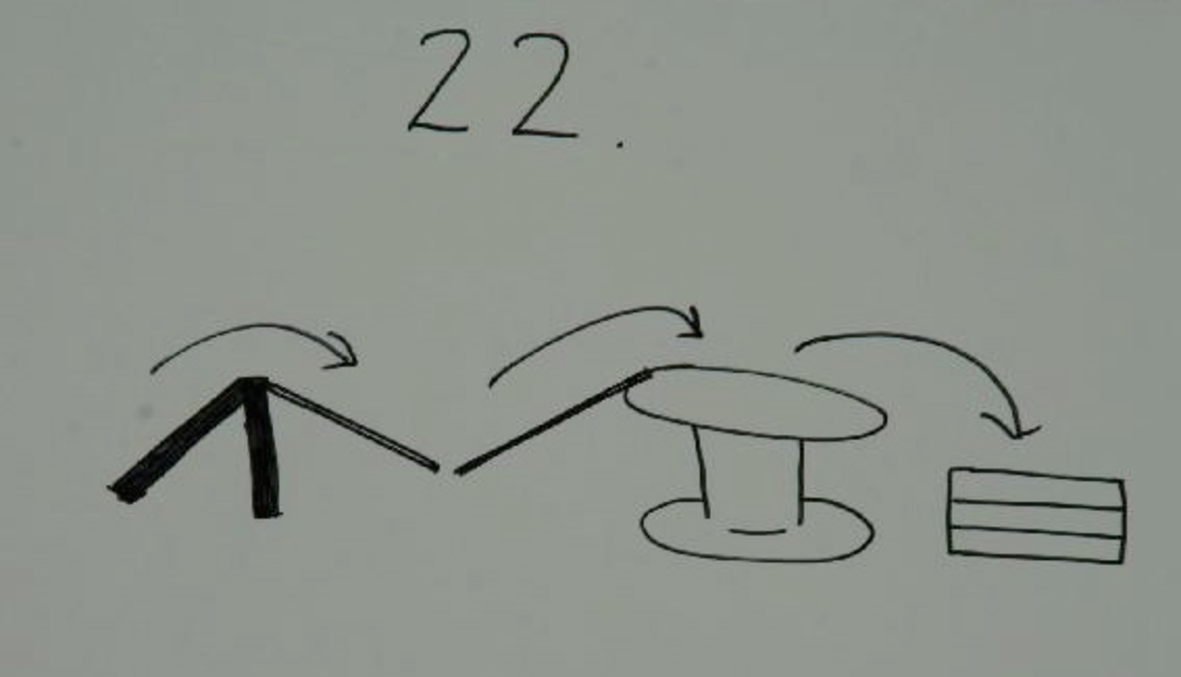
\includegraphics[scale=0.3]{trials} }\\
\hline
\end{tabular}

To make it easier to describe sections, label major obstacles with numbers and/or letters. 
These should be clearly visible at a distance. 
Plastic laminated cards with letters or numbers are good because they can be re-used at other competitions.

One good strategy is to label all boxes with numbers, and all beams with letters. 
This makes it much easier to include section descriptions such as ``ride from Beam A to Box 6, without touching the ground.''
Section instructions should not require or prohibit a rider from using certain techniques to complete a section. 
For example, the instructions must not prohibit the use of pedal grabs or bash guards in order to increase the challenge.

\subsection{Section Difficulty}
The range in difficulty of sections should correspond to the range in ability levels of the participants. 
The easiest sections should be cleanable by all participants after one or two attempts, and the harder sections should require multiple attempts by the best riders.

It is highly recommended to include one or two sections that are so difficult that they may only be cleaned by one rider, or not at all. 
This will help prevent ties for first place, and may also help to increase the technical standards of the sport if a rider succeeds in doing something that has never been done before.

\subsection{Course Planning: Location And Materials}
It is most important to make maximum use of available resources. 
Prior planning and proper site selection are essential.
Expect to take at least one day to set a course for a major competition, plus time to assemble the raw building materials.

If possible, select a course location with an abundance of natural obstacles, or features that can be incorporated into human-constructed obstacles. 
It cannot be overstated that is much easier to make use of what is already there, rather than constructing new obstacles.

Sections may be set on natural features such as bedrock, boulders, logs, and hill slopes, and/or constructed from stacked pallets, railings, truck tires, junkyard cars, obstacles constructed from lumber, or any other material at hand. 
Often it is good to combine natural features with human-constructed obstacles.

It is highly recommended to also build a basic practice area to be set up outside of the competition area. 
This can consist of a small number of random obstacles, and is important for warm-up and to reduce the temptation to ride on the course prior to the event.

Make sure that there is plenty of extra building material (tools, screws, and raw materials) on hand to repair sections damaged during the event.

\subsection{Course Design}
Sections should differ substantially from each other and test a variety of hopping and rolling techniques. 
Often, it is a good idea to mentally make a list of the different techniques in trials, and design sections that test each of them separately or in combination.

The course layout is controlled mainly by the available resources.
If there are abundant natural obstacles, design sections around the most obvious natural features.

For either natural or artificial sections, a good way to maximize resources is to first construct several major structures that can be used as centerpieces, or hubs, and then design sections that center around these hubs. 
For example, a car, spool, or large boulder could serve as a hub, surrounded by smaller structures that lead onto and over the hub in different ways.

Building centralized hubs rather than independent sections allows for high concentrations of sections on less building material.
Unlike conventional bike trials, it is not a problem to design overlapping sections, although sometimes it may cause delays as riders wait for their turn. 
Usually a combination of hubs and independent sections is best.

It is extremely important to design sections that are durable enough that they do not break or change during the competition time period.

Overall, a course should not favor left or right handed riders, or riders with right- or left-foot-forward hopping stances.
For example, the Course Setter should include sections requiring hops to both the right and to the left.

It is best to design sections that provide challenge without undue risk. 
Typically the best-designed sections include moves that test balance and precision, rather than moves that are difficult only because they are big. 
For example, rather than constructing a big, basic drop or gap between easy terrain, increase the difficulty of the takeoff or landing areas by making them smaller or off-angle. 
It is strongly recommended to avoid building any drops to hard, flat ground that are greater than 1.5m height.

There is no requirement that riders exit a section while in full control of their cycle. 
Consequently, a well-designed section should force riders to be in control in order to finish---it should not be common for riders to fall across the finish line. 
The easiest way to do this is to include at least 2 meters of easy ground between the last hard obstacle and the finish line.

A photo album of previously constructed sections is located at www.krisholm.com/sections.

\subsection{Time And Space-Saving Strategies}
If building material is extremely limited and there are very few participants, an alternative competitive strategy is to create an elimination round, instead of setting an entire course.

A small number of sections are set (as little as 1 section at a time), and riders attempt all sections. 
Any rider who cannot clean an obstacle after multiple attempts is eliminated. 
Then a second set of section(s) is set, and the process repeated until only one rider can clean the section(s). 
This option works with minimal resources but should be regarded as a last resort.
\part{Hockey}
\parttoc
\singlechapter{Hockey \label{chap:hockey}}

Attention must be drawn to the safety of the players and spectators.
Thus, the safety rules have to be obeyed strictly and all equipment must be in good condition.
These rules cannot cover every situation.
Teams have to agree on a specific amount of elbow-room before playing.
The different backgrounds of the players and the conditions of the location have to be considered.
Fairness of everyone involved is vital.

\section{Playing Field}

\subsection{Dimensions}

\setlength{\unitlength}{0.1mm}
\begin{picture}(1600,1000)

% field:
\thicklines
\put(850,475){\oval(1300,750)}

% 6.50m line:
\put(400,100){\line(0,1){30}}
\put(400,160){\line(0,1){30}}
\put(400,220){\line(0,1){30}}
\put(400,280){\line(0,1){30}}
\put(400,340){\line(0,1){30}}
\put(400,400){\line(0,1){30}}
\put(400,460){\line(0,1){30}}
\put(400,520){\line(0,1){30}}
\put(400,580){\line(0,1){30}}
\put(400,640){\line(0,1){30}}
\put(400,700){\line(0,1){30}}
\put(400,760){\line(0,1){30}}
\put(400,820){\line(0,1){30}}

% center line:
\put(850,100){\line(0,1){750}}

% 6.50m line:
\put(1300,100){\line(0,1){30}}
\put(1300,160){\line(0,1){30}}
\put(1300,220){\line(0,1){30}}
\put(1300,280){\line(0,1){30}}
\put(1300,340){\line(0,1){30}}
\put(1300,400){\line(0,1){30}}
\put(1300,460){\line(0,1){30}}
\put(1300,520){\line(0,1){30}}
\put(1300,580){\line(0,1){30}}
\put(1300,640){\line(0,1){30}}
\put(1300,700){\line(0,1){30}}
\put(1300,760){\line(0,1){30}}
\put(1300,820){\line(0,1){30}}

% breadth:
\put(100,400){\vector(0,-1){300}}
\put(100,550){\vector(0,1){300}}
\put(80,100){\line(1,0){40}}
\put(120,850){\line(-1,0){40}}

% length:
\put(650,950){\vector(-1,0){450}}
\put(1050,950){\vector(1,0){450}}
\put(1500,930){\line(0,1){40}}
\put(200,970){\line(0,-1){40}}

% 6.50m marks:
\put(400,475){\circle*{15}}
\put(1300,475){\circle*{15}}

% center mark:
\put(850,475){\circle*{15}}

% corner marks:
\put(300,200){\circle*{15}}
\put(300,750){\circle*{15}}
\put(1400,200){\circle*{15}}
\put(1400,750){\circle*{15}}

% goal line:
\put(300,400){\line(0,1){30}}
\put(300,460){\line(0,1){30}}
\put(300,520){\line(0,1){30}}
\put(250,400){\line(0,1){150}}
\put(300,400){\line(-1,0){50}}
\put(300,550){\line(-1,0){50}}

% goal line:
\put(1400,400){\line(0,1){30}}
\put(1400,460){\line(0,1){30}}
\put(1400,520){\line(0,1){30}}
\put(1450,400){\line(0,1){150}}
\put(1400,400){\line(1,0){50}}
\put(1400,550){\line(1,0){50}}

% distances:
\put(1300,650){\vector(1,0){100}}
\put(1400,650){\vector(-1,0){100}}
\put(1400,630){\line(0,1){40}}

% distances:
\put(1400,300){\vector(1,0){100}}
\put(1500,300){\vector(-1,0){100}}
\put(1400,280){\line(0,1){40}}

% text:
\put(900,650){\makebox(0,0)[l]{ center line }}
\put(900,650){\vector(-1,-1){50}}
\put(460,675){\makebox(0,0)[l]{ corner mark }}
\put(460,675){\vector(-2,1){150}}
\put(300,620){\makebox(0,0)[c]{ goal area }}
\put(460,530){\makebox(0,0)[l]{ 6.50~m mark }}
\put(460,530){\vector(-1,-1){50}}
\put(900,530){\makebox(0,0)[l]{ center mark }}
\put(900,530){\vector(-1,-1){50}}
\put(460,230){\shortstack{corners\\rounded or\\beveled}}
\put(450,230){\vector(-2,-1){200}}
\put(700,50){\makebox(0,0)[l]{ side line }}
\put(1250,400){\makebox(0,0)[r]{ goal line }}
\put(1250,400){\vector(2,1){150}}
\put(1250,300){\makebox(0,0)[r]{ 6.50~m line }}
\put(1250,300){\vector(1,-1){50}}
\put(1530,550){\shortstack[l]{ground\\line}}
\put(850,950){\makebox(0,0){length: 35 -- 45~m}}
\put(100,475){\makebox(0,0){\shortstack{breadth:\\20 -- 25~m}}}
\put(1300,700){\makebox(0,0)[l]{ 6.50~m}}
\put(1500,350){\makebox(0,0)[r]{2.50~m }}
\end{picture}

The field has a length of 35 to 45 meters and a breadth of 20 to 25 meters.
It is surrounded by barriers.
The corners are rounded or beveled.

\subsection{Goals}
The posts are 2.50 m in from the ends of the playing field (ground lines), ensuring that the players can go behind them.
The inside dimensions of goal openings are 1.20 m high and 1.80 m wide.
The goals must be made in such a way that the ball cannot enter through the rear or sides. The goals must not have sharp, pointed or protruding parts.

\subsection{Markings}
The center line divides the field into two equal halves, and the center mark is in the middle of the center line.
There are marks in front of each goal at a distance of 6.5 m.
The goal lines connect the posts on the ground.
The corner marks are on the extension of the goal lines, 1.0 m in from each side line.
The 6.5 m lines are parallel to the goal lines and run through the 6.5 m marks.
The goal areas are between the 6.5 m lines and the ends of the field.

\section{Teams}

\subsection{Number Of Players}
A team consists of five players (plus substitutes).
Substituting one player for another is possible at any time.
It is not necessary to indicate it to the Referee.
The new player must enter the field where the other exits it.
Each player can be the goalkeeper at any time.
The goalkeeper has no special rights.
To take part in a game, a team must have at least three players.

\subsection{Clothing}
Shoes must be worn.
All players of a team must wear shirts of the same color.
The color must be clearly different from the opponent's color.
At tournaments and other large events each team should have two different colored sets of shirts.

Clothing suggestions for comfort and safety:
\begin{itemize}
\item Cycling shorts and kneepads, or long pants
\item Gloves
\item Short shoe laces, or laces tucked in
\item Helmet and dental protection
\item Definitely no jewelry (watches, necklaces, earrings)
\end{itemize}

\section{Equipment}

\subsection{Unicycles}
The maximum wheel size is 618~mm (24$"$).
The unicycles must not have sharp or protruding parts anywhere that might cause injuries.
This refers especially to quick-release levers and bolts.
The pedals must be plastic or rubber.

\subsection{Sticks}
All sticks legal for playing ice-hockey or floorball (apart from those for the goalkeeper) can be used.
Cracked or splintered sticks must be taped or repaired before play.
An upper end made of rubber is recommended.

\subsection{Ball}
A ``dead'' tennis ball that reaches 30 percent to 50 percent of its original height after bouncing onto concrete is used.
Alternatively, a street hockey ball can be used.
The choice is made by the hosting organization if the opposing teams do not agree on which ball to use.
The chosen type of ball must be announced well in advance of the competition, and must be obtainable in all participating countries.

\section{Penalties}
In every instance of a violation of the rules the Referee must penalize the offending team, unless the Referee decides not to interrupt the game (advantage).

\subsection{Free Shot}
The free shot is the standard penalty for all violations of the rules.
It is applied in all cases except for those explicitly mentioned in sections \ref{subsec:hockey_penalties_65m}-\ref{subsec:hockey_penalties_bully}.
The free shot is executed from the point where the violation was done.
Exceptions: If a team gets a free shot within the opponents' goal area, the free shot is done from the closest corner mark (corner shot).
If a team gets a free shot within their own goal area, the free shot is done at a distance of 1 m in front of the goal line (goalkeeper's ball).

The free shot is indirect.
The player executing the free shot may only touch the ball once.
Then another player has to touch the ball.
Opposing players must keep a distance with their unicycles and their sticks of at least 2.0 m from the ball.

\subsection{6.5 M \label{subsec:hockey_penalties_65m}}
If legal playing would have led to a direct chance to score a goal, a ``6.5 m'' is given.
This includes fouls outside the goal area.
The ball is placed at the 6.5 m mark.
A player of the defending team goes to the goal and must sit with the bottom of the wheel of their unicycle within 0.5 m of the goal line.
The other team chooses a player to shoot the 6.5 m.
All other players must leave the goal area.
After the Referee's whistle the goalkeeper must ride the unicycle freely and not rest on the goal.
If no goal is scored, play continues as soon as the ball touches the post, the keeper touches the ball or the ball crosses the extended goal line.

\subsection{Penalty Goal}
If the defending team prevents a goal from being scored through an illegal play of the ball and if, in the opinion of the Referee, the ball was traveling directly toward the goal and would definitely have entered the goal without being touched by another player, a penalty goal may be awarded.
In this case the attacking team is awarded a goal.
If there is any doubt as to the certainty of a goal, a 6.5 m must be awarded as described in section \ref{subsec:hockey_penalties_65m}.

\subsection{Bully \label{subsec:hockey_penalties_bully}}
Whenever the game needs to be resumed without penalizing one of the teams, this is done with a bully (face off).
For the bully, the Referee drops the ball between two opposing players.
Playing starts when the ball touches the ground.
A bully during the game is executed where the ball was when the game was interrupted. 
Exception: Within the goal area, the bully is always executed near one of the corner marks.

\subsection{Penalty Box}
The Referee can send a player off the field for two minutes, five minutes or for the remainder of the game.
This is done in the case of unsporting behavior and also for intentional or dangerous disregard of the rules.
While a player is in the penalty box, the team may not substitute a replacement for that player.

\section{Course Of The Game}

\subsection{Game Duration}
The play time is given by the playing schedule.
It is a relative play time.
The time only stops if the Referee requests a time out.
The teams change sides during the break.
At the start of each period, all players must be in their own half of the field.
Each period starts with a bully at the center mark.
If the game ends in a draw and a decision is necessary, play is continued for ten more minutes: five-minute break and change sides, five minutes of play, change sides without a break and five more minutes of play.
If it's still a draw, a decision is reached with a penalty shootout.

\subsection{Penalty Shootout}
Three of the players from each team get one penalty shot each.
If it is still a draw, each team shoots one more penalty until there is a decision.
It is possible that one player can make more than one shot.
However, in all cases at least two other players have to make a shot before the same player can shoot again.

For the penalty, all players except for a defending goalkeeper leave the corresponding half of the playing field.
The goalkeeper must be close to the goal line, at least until the attacking player has had contact with the ball.
The Referee places the ball on the center point and the player taking the shot will, after the whistle of the Referee, play the ball from there, trying to score a goal.
The ball must be kept in motion towards the goal line (no backwards movement allowed) and once it is shot, the play shall be considered complete.
No goal can be scored on a rebound of any kind (an exception being the ball off the goal post, then the goalkeeper and then directly into the goal), and any time the ball crosses the goal line, the shot shall be considered complete.

\subsection{Riding The Unicycle}
The player has to be riding the unicycle freely.
He or she may use the stick as support but must not rest on the goal or the wall or something similar.
It is not sufficient to release the goal only quickly for the time while the goalkeeper takes part in the game.
A short support on the wall to avoid a dismount can be tolerated.
A player who is falling off the unicycle may take part in the game until touching the ground.
A remounting player must sit on the seat and have both feet on the pedals before participating in the game again.
If a player who is not riding a unicycle shoots into their own goal, the advantage rule applies for the attacking team and the goal is valid.

\subsection{Obstacle}
A player who is off the unicycle must not be an obstacle for opponents.
The player is considered an obstacle if the player, the unicycle or stick is hit by the ball and also if an opponent cannot move around freely.
The player should remount at the same spot, but if necessary move out of the way of play first.

\subsection{Contact With The Ball}
The stick, the unicycle and the whole body can be used to play the ball.
It all counts as a contact.
Players are allowed to play the ball with the body twice in a row only if one of the contacts is passive.
When the ball is played with the body, the player must not catch or otherwise hold the ball and the contact with the ball should be instantaneous.
For arms and hands see also section \ref{subsec:hockey_goal-shots_with-arms-or-hands}.

\subsection{Start and Stop}
Starting and resuming the game is always initiated by the Referee's whistle.
When the Referee blows the whistle during the game, it is interrupted immediately.

\subsection{Restart After A Goal}
After a goal, the non-scoring team gets the ball.
All players must go to their own half.
After the Referee's whistle, the game resumes when the ball or a player of the team in possession crosses the center line.
It is legal to directly shoot a goal after passing the center line, for example without passing the ball to another player first.

\subsection{Ball Out Of Bounds}
If the ball leaves the field, the team opposite to that of the player who last touched it gets a free shot or a corner shot, depending where the ball went out.
The free shot is done 1.0 m in from the side line.

\subsection{Moving The Goal}
If a player moves the goal, the game is interrupted and the opposing team gets a free shot.

\subsection{Ball In Spokes}
If the ball gets stuck between the spokes of someone's unicycle, the opposing team gets a free shot (not a 6.5m penalty).

\section{Fouls}

\subsection{General Considerations}
All players must take care not to endanger others.
The game is contactless: the opponents and their unicycles may not be touched.
The players must take care not to hit an opponent with their stick, especially after a shot.
Only in the vicinity of the ball, they may touch an opponent's stick with their stick to block them.
However, this contact may not be hard.
It is illegal to turn the blade of the stick upside down in order to hook into an opponent's stick.
Raising the opponent's stick is allowed in principle, if not done using exaggerated roughness.
If the opponent's stick is raised above the height of their hips, it is always considered exaggerated roughness.

\subsection{Right Of Way}
To keep the game going, rule violations that do not influence the course of the game should not be penalized.
The following rules apply when riders come into contact with each other:
\begin{itemize}
\item No player may endanger another player by forcing them to give way (for example, to push them toward the wall).
\item A player who is idling or resting on the stick must be evaded.
\item The leading of two players riding next to each other may choose the direction of turns. If both are evenly side-by-side, the one having the ball may choose the direction.
\item If two players are approaching each other directly or at an obtuse angle, the one with the ball has the right of way.
\item In all cases not mentioned above, it is up to the Referee to make a decision.
\end{itemize}

\subsection{SUB (Stick Under Bike)}
A player who holds his or her stick in a way that someone else rides over or against it is committing a foul, regardless of intention.
According to the situation the player who was ``subbed'' is given either a free shot or a 6.5 m.

\subsection{SIB (Stick In Bike)}
If a stick gets into the spokes of an opponent, the holder of the stick is committing a foul regardless of intention.
According to the situation the player who was ``sibbed'' is given a free shot or a 6.5 m.

\subsection{Insults}
A player must not insult the Referee or other players.

\subsection{Intentional Fouls \label{subsec:hockey_fouls_intentional-fouls}}
Intentional fouls are considered to be unsporting behavior.
The respective player is sent off the field for at least 2 minutes.

\section{Goal Shots}

\subsection{Goal Shot With Arms Or Hands \label{subsec:hockey_goal-shots_with-arms-or-hands}}
A goal is disallowed if scored with arms or hands.
The defending team gets a free shot (goalkeeper's ball).
This rule does not apply if the ball is shot into one's own goal.

\subsection{Long Shot}
A goal is disallowed if the last contact with the ball was made when the ball was in one's own half.
The defending team gets a free shot (goalkeeper's ball).
This rule does not apply if the ball is shot from the opponents' half into one's
own goal.

\subsection{Ball In The Outside Of The Net}
If the ball becomes lodged in the outside of the goal net, or if the ball entered the goal through the net from the side the back through a hole in the net, a free shot is given against the team whose player last played the ball.

\section{Safety Rules}

\subsection{Throwing Sticks}
A player who intentionally drops or throws his or her stick is sent off the field for at least 2 minutes, at the discretion of the Referee (section \ref{subsec:hockey_fouls_intentional-fouls}).
Also, the opposing team gets a 6.5 m.

\subsection{Top Of The Stick}
The upper end of the stick must always be covered with one hand to avoid injury to other players.
A brief removal of the upper hand from the stick to play the ball with that hand is acceptable provided that this is done in a safe manner.

\subsection{The Lower End Of The Stick}
The lower end of the stick must always be below the players' hips to avoid injury to other players.
Exception: In direct vicinity of one's own goal, the lower end of the stick can be raised as high as the crossbar of the goal.

\subsection{Exaggerated Roughness}
Exaggerated roughness can lead to injuries and must therefore be avoided.

\section{Referee Rules}

 \subsection{Members Of The Board Of Referees}
\begin{wrapfigure}{r}{0.5\textwidth}
\begin{center}
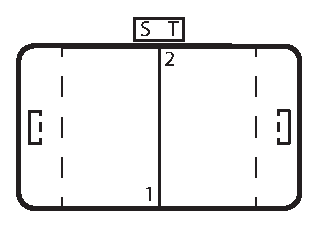
\includegraphics[scale=0.75]{referees}
\end{center}
\end{wrapfigure}
 The Board of Referees consists of:
\begin{itemize}
\item First Referee (1) 
\item Second Referee (2)
\item Secretary (S)
\item Timer (T)
\end{itemize} 

\subsection{The Referees}
The two Referees are positioned one on each side.
They try to stay close to the ball.
They should not ride a unicycle.
The clothes of the Referees must be of different color than those of the players.
Both Referees are responsible for checking all violations of the rules.
The first Referee has three additional tasks:
\begin{itemize}
\item The First Referee overrules the Second Referee, if they disagree.
\item The First Referee restarts the game after every interruption by a long blow of the whistle.
\item The First Referee drops the ball in for the bully.
\end{itemize}

\subsection{The Secretary}
The Secretary sits at the desk and takes care that the scoreboard always shows the current score.
After a goal the Secretary seeks eye contact with the First Referee to check if the goal is declared valid or not.
After the end of the game the Secretary writes the final score into the report.

\subsection{The Timer}
The Timer checks the time of play with a stopwatch.
The watch is started whenever the Referee starts the game by blowing the whistle.
At the end of each period, the Timer stops the game by blowing the whistle.
The Timer also stops the time whenever the Referee requests a time out.

\subsection{Before The Game}
Before the game, the Referees assemble all players on the field (including substitutes).
They check the following:
\begin{itemize}
\item Are the colors of the shirts of the players clearly different?
\item Did all players take off their watches and jewelry that might injure others?
\item Is the ball suitable?
\item Are the unicycles and sticks orderly, without sharp, pointed or protruding parts that might injure others?
\item They explain to the players how strictly they will interpret the rules.
\item If necessary, they tell the players how long the game will be and also if there is extended time in case of a draw.
\end{itemize}

\subsection{General}
The game is interrupted by a short and loud blow of the whistle.
If any players don't hear the whistle, it is necessary to blow the whistle again.
It is not possible to let the game continue after blowing the whistle.

The Referees should set the tone through their positive and calm appearance.
Decisions are explained upon request but they are not discussed with the players.
In an unclear situation, the Referees can ask the players before making a final decision.

Neither the Referees nor the Timer or Secretary may be distracted from the game.
Most of all, they must not talk with the spectators during the game.

If two violations of the rules occur back-to-back, only the first one is penalized.
Exception: Unsporting behavior should be penalized even after the game has been interrupted.

After a goal, the Referee waits until both teams are back in their own halves and ready to continue.
Only then, the first Referee starts the game by blowing the whistle.

If the teams start to play even though the game had not been started by the Referee, it is stopped immediately by two or more quick consecutive blows of the whistle.

To apply the advantage rule, the Referee makes the normal sign for a free shot with one arm pointing in the direction of play of the team who has the advantage.
In addition, the Referee may shout ``Advantage'' or ``Go ahead!'', but does not blow the whistle.
The end of advantage play should be signified, either by blowing the whistle to give a free shot for the original foul in the case where no advantage was gained, or by lowering the arm again and/or shouting ``Advantage over''.

After each interruption of the game the Referee briefly explains the decision.
In addition the corresponding hand sign is shown.

When two or more players fall and it is unclear whether a foul occurred, the Referees can interrupt the game and then continue it with a bully.
This prevents that even more players are drawn into the situation.

The Referees suspend the game if an injury occurs.
Afterwards, a free shot is given to the team that was in possession of the ball at the time of the interruption.
If it is unclear who was in possession, the game is continued with a bully.

\subsection{Referee Hand Signs}
\renewcommand{\arraystretch}{1.5}
\begin{longtable}{|p{3cm}|p{11cm}|}

\hline
\raisebox{-1\height}{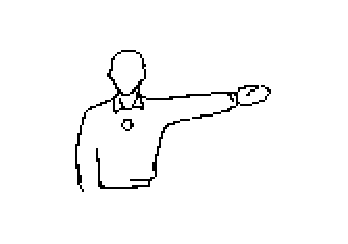
\includegraphics[scale=0.6]{1_h}}
&
\textbf{``Free shot''}

Point with the extended arm in the direction of play.

This sign is also used to indicate the advantage rule. \\
\hline
\raisebox{-1\height}{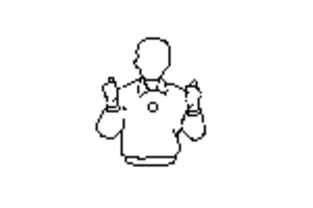
\includegraphics[scale=0.6]{2_h}}
&
\textbf{``Bully''}

Hold both thumbs up.  \\
\hline
\raisebox{-1\height}{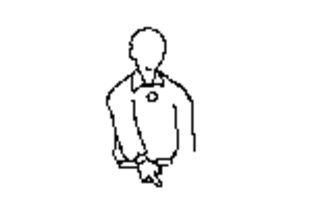
\includegraphics[scale=0.6]{3_h}}
&
\textbf{``6.50 m''}

Point with the index finger to the 6.50 m point. \\ 
\hline
\raisebox{-1\height}{
\includegraphics[scale=0.6]{4_h}}
&
 \textbf{``No Foul''}

Extend both arms horizontally.

This sign is used to indicate that there was no foul in a critical situation. It is not used in conjunction with a blow of the whistle. \\ 
\hline
\raisebox{-1\height}{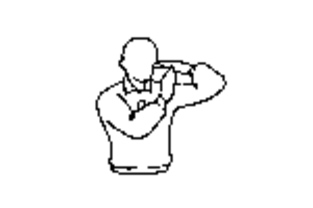
\includegraphics[scale=0.6]{5_h}}
&
\textbf{``Time out''}

Form the letter ``T'' with both hands.

The game is interrupted for example if a player is injured or if the spectators disturb the game. \\ 
\hline
\raisebox{-1\height}{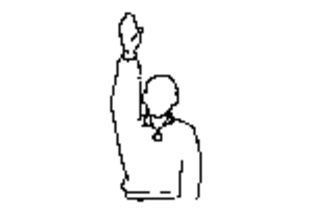
\includegraphics[scale=0.6]{6_h}}
&
\textbf{``Goal''}

Point upwards vertically with one arm.

The Referees should check here that the secretary notes the goal.
To control this it may be useful for the Referees to write down the score themselves. \\ 
\hline
\raisebox{-1\height}{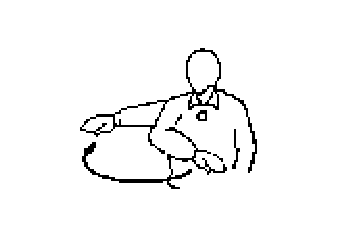
\includegraphics[scale=0.6]{7_h}}
 &
 \textbf{``No goal''}

Move the flat hand horizontally (palm pointing down).

With this hand sign a goal shot is declared invalid.
This is for example the case if the ball was last touched by hand or arm, in case of a long shot, if the ball entered the goal through the net from the outside, or if the game had already been stopped before the ball entered the goal.
The Referees should check here that the Secretary does not inadvertently count the invalid goal.\\ 
\hline
\raisebox{-1\height}{
\includegraphics[scale=0.6]{8_h}}
&
\textbf{``High stick''}

Hold clenched fists next to each other above the head. \\ 
\hline
\raisebox{-1\height}{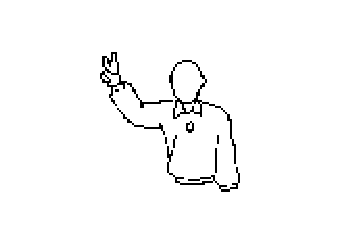
\includegraphics[scale=0.6]{9_h}}
&
\textbf{``Penalty box for 2 minutes''}

and also 

\textbf{``Two consecutive plays with the hand''}

Spread and raise two fingers.  \\ 
\hline
\raisebox{-1\height}{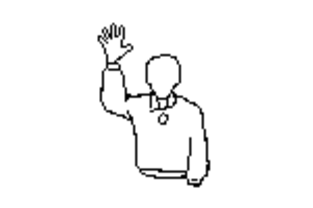
\includegraphics[scale=0.6]{10_h}}
  &
\textbf{``Penalty box for 5 minutes''}

Spread and raise five fingers.\\
\hline
\end{longtable}
\renewcommand{\arraystretch}{1}


In IUF competition, unicycle basketball is played using the international rules for regular basketball with a few changes.\\
The items below, in combination with standard international basketball rules, are what are used for Unicon competition.
\section{Unicycles}
The maximum wheel size is 640mm (25.2”). The unicycles must not have sharp or protruding parts anywhere that might
cause injuries. Quick-release levers and bolts, for example, must be folded back and not excessively long. The pedals must
be plastic or rubber.
\section{Violations}
A violation occurs when the player breaks one of the rules of Basketball. A violation results in the awarding of the ball to
the opposing team. Examples of violations include traveling, double dribble, backcourt violation, palming the ball, and
stepping out of bounds.
\section{Fouls}
A foul is an illegal action that can be committed by a player from one team against a player from the opposing team. If
contact occurs beyond what is deemed to be reasonable, or if a player thereby obtains an unfair advantage from it, a foul is
committed. Examples of fouls include pushing, tripping, striking or holding an opposing player and unsportsmanlike
conduct. A foul results in the awarding of the ball to the opposing team and/or free throws.
\section{Steps And Traveling}
A traveling violation occurs when a player holding the ball steps in excess of the prescribed limits. A step is a half
revolution of the wheel; meaning that each wheel revolution is the equivalent of two steps because pedaling with one leg
only moves the wheel half a revolution. After a player establishes a pivot foot (the bottom foot of an idle), the player may
not switch the idle foot or take a step unless he begins dribbling. If a player is in the act of passing or shooting the ball,
then the player is allowed to take one full step without dribbling.
\section{Idling, Twisting and Hopping}
Idling is equivalent to the pivot foot and therefore is allowed. Twisting, where the pedals stay at the same height, while
you move the unicycle left and right is also considered your pivot foot, and therefore allowed. The player must also stay
within a one-meter radius from the point where the idling or twisting started. A player may not hop (jump up and down
repeatedly with the unicycle) while holding the ball. Hopping while dribbling is permitted.
\section{Mounted Player}
The player can only play the ball while mounted on the unicycle. A player has established position on the unicycle
("mounted") when the player is sitting on the seat, with both feet on the pedals, and is not touching anything else for
support. Once a player is mounted, the player is considered mounted until some part of his body touches the ground. The
player throwing the ball inbound must be mounted.
\section{Unmounted Player}
If contact is made between the ball and an unmounted player or unicycle, the ball shall be awarded to the other team.
Referees may allow incidental contact between the ball and an unmounted player or unicycle if such contact does not
disrupt the flow of the game. An unmounted player must move himself and his unicycle out of the way as soon as possible
without disrupting the flow of play. If not possible, the player must leave the unicycle where it lands until it can be
retrieved without being disruptive. A violation will result in an obstruction foul.\\
An unmounted player's unicycle is considered part of the player. For the purposes of fouls, a stationary riderless unicycle
is considered to have established position; a riderless unicycle that is moving is considered to be out of control. Thus, if
another player is hit by a moving abandoned unicycle, a foul will be called. If an unmounted player intentionally attempts
to play the ball or impede another player, a technical foul will be called.
\section{Four Second Zone}
The three-second zone becomes the four-second zone.
\section{Contact of the Ball with a Unicycle}
It is a violation for a player to intentionally strike or stop the ball with any part of his unicycle or leg, however, incidental
contact with a player's unicycle or legs is not a violation. As long as the player is in contact with the unicycle, riding or
not, it is considered part of a player when a ball bounces out of bounds off the unicycle. If this happens the other team
receives possession of the ball.
\section{Ball on Floor}
Any player may pick up a ball that is rolling or stopped on the ground. This can be dangerous, so care must be taken not to
foul a player that is bent over to pick up the ball. A player may stop a rolling ball with their hand or push a stopped ball to
a teammate to pick up.
\section{Referee Signals}
\textbf{Administrative signals:}
\textbf{Scoring signals:}
\textbf{Violation signals:}

\singlechapter{Skill Levels \label{chap:skill}}

\section{Purpose of the Skill Levels}
These achievement skill levels have been complied from years of research and surveys among unicyclist from all over the world.
They are intended to encourage unicyclists to progress at an even pace over a wide variety of unicycling skills.
These levels are not connected to the competition rules, other than in descriptions of how the skills are to be performed.
Skill levels are useful for helping riders determine a sequence of skills to learn, and to give them ideas for things to try.

\section{Testing of the Skill Levels}

\subsection{Official IUF Skill Level Testers}
The IUF Executive Board authorizes official level testers every two years at Unicon, the International Unicycling Championships and Convention, and at miscellaneous times throughout the year at Regional Clinics.
Any member of the IUF has the potential of being an official tester through the annual IUF Official Skill Level Clinic or Regional Clinic, both administered by a representative appointed by the IUF executive board.
Any member of the International Unicycling Federation may test Level 1 through 3 without going through certification.

\subsection{Becoming an Official Tester}
To become an official skill level tester, an IUF member needs to:
\begin{itemize}
\item Attend the Biannual Skill Level Clinic, offered three to five times during Unicon every two years, or attend a regional clinic, offered by miscellaneous officials throughout the year.
\item Fill out the Skill Level Tester Confirmation Form, available at the clinics.
\item Agree to follow all rules and guidelines presented in the clinic.
\end{itemize}


\subsection{IUF Biannual Skill Level Clinic and Regional Clinics}
The IUF Biannual Skill Level Clinic is a thorough explanation and demonstration of the 10 Official Skill Levels and corresponding rules for potential IUF Official Skill Level Testers.
This clinic will assist in creating a uniform standard of level testing throughout the world.
The Regional Clinics contain the same information and certification program as the Biannual Clinics but are taught at various times throughout the year, to be published on the IUF website.

The purpose for future IUF Skill Level Testers to attend the Biannual Skill Level Clinic or Regional Clinic is to:
\begin{itemize}
\item Qualify to become an Official IUF Skill Level Tester.
\item Be able to recognize and understand all skills in the skill levels.
\item Be able to test at a very accurate, consistent, and professional level.
\item View demonstrations of all skills in levels 1 through 10.
\item Have unanswered questions presented, discussed, and resolved.
\item Be able to understand all rules stated on the skill level card as well as in the IUF Official Rulebook, section 8.
\end{itemize}
Other Clinic Information:
\begin{itemize}
\item Length of each Level Clinic will vary, with an approximate time allotment of one hour.
\item Leader of each clinic will be available following each clinic to answer any unanswered questions.
\end{itemize}

\subsection{Skill Level Tester Confirmation Form}
In addition to attending the Biannual Skill Level Clinic or Regional Clinic, potential testers are also required to sign the Skill Level Tester Confirmation Form, which are available upon completion of the clinic and tutorial.
By signing this document, the potential tester agrees to all rules and responsibilities presented in chapter \ref{chap:skill} of the IUF Rulebook.
Signing also confirms their decision to become certified as an IUF Official Level Tester.
Each potential tester will also be asked to state the level he/she desires to be able to test to.
All completed forms will be examined and considered by the IUF Skill Level Director and within 30 days of signing, an email certification will be sent to all potential testers.
From the day the certification is sent, potential testers have up to 15 days to appeal to the IUF Executive Board for a re-evaluation (i.e. more levels desired to test than actually granted).

\subsection{Responsibilities of an Official Skill Level Tester}
Once an IUF member is confirmed as an Official Skill Level Tester, he/she is required to:
\begin{itemize}
\item Submit all passed skill levels to the IUF by sending them to the current International Skill Level Director's email address.
Submit the name of the person tested, the level(s) passed, the date each level was passed, and the name(s) and country number(s) of the level tester (if applicable).
All levels passed by members are stored in the IUF database.
The level tester must be certified to test the level of the submitted passed skill level.
For Level 8 and above, two certified testers for Level 8 and above must be submitted for verification.
Exceptions may be made by the IUF executive Board on a case-by-case basis, prior to testing.
\item Attend the Biannual Skill Level Clinic and/or Regional Clinic every other year for testing renewal.
This allows for each tester to refresh his/her knowledge as well as get updated on newly passed guidelines.
Certified skill level testers may also be granted permission to teach mini skill level clinics within their country's national convention, clubs or others not within a club, as determined by the IUF.
\item Follow completely and accurately all rules and guidelines presented in section 8 of the IUF Rulebook.
Any questions or concerns must be directed towards the International Skill Level Director immediately.
Failure to do so will result in restrictions and/or loss of ability to test.
\item The IUF will provide testers with a standard template for certificates that can be printed out and given to riders upon completion of each level.
\end{itemize}

\subsection{Restrictions for Official Level Testers}
Questionable knowledge will be confirmed by the International Skill Level Director through personal discussions, practice test situations, and/or outside connections to the potential tester prior to level testing confirmation.
\begin{itemize}
\item Testers are unable to test their own family members.
\item Testers must be at least 14 years old to qualify.
\item Riders and non-riders can test to the level in which he/she has the greatest proven knowledge (as decided by the International Skill Level Director).
\end{itemize}

\subsection{Recognition of Skill Levels}
All Skill Levels successfully passed are to be submitted to the IUF Skill Level Director every six months.
Once submitted, the IUF Skill Level Director will verify the levels.
Any Official Skill Level Tester from any country may test levels, as long as the guidelines highlighted in the IUF Rulebook, Chapter \ref{chap:skill}, are accurately followed.
National organizations must recognize all verified Skill Levels by the IUF independent of the country in which specific levels.

\section{Guidelines of the Skill Levels}

\subsection{General}
\begin{itemize}
\item Rider must perform all skills in the level at the first attempt except for three skills maximum, which must be performed at the second attempt.
This means only one mistake for each skill and maximum of three mistakes per
level.
\item All preceding levels must be passed prior to testing for a higher skill level.
\item All skills (except mounts) must begin and end with the rider sitting on the seat, feet on the pedals, and riding in control for at least three revolutions before and after each skill (complete cycles of the wheel).
\item Skills in each level can be performed in any order.
\item Rider cannot use any external aids during any part of the test for any level.
These include walls, other people, etc.
\item Within a specific level test, the rider must use the same unicycle to pass all skills within that level.
\item All skills within a level must be performed within one hour of the beginning of the test.
\item During the test, the rider may not practice any skills for that level.
(They should not be allowed on their unicycle unless they are certainly testing!)
\item Riders may only test once per day.
Exceptions will be given by consent of the IUF's Executive Board.
\item Interference (i.e. another rider obstructing the rider's path) to a testing rider is up to the discretion of the tester(s).
If the tester rules interference, the rider has another opportunity to complete the interfered skill.
Interference will be based upon visual evidence, outside witnesses, and the integrity of the rider.
\end{itemize}

\subsection{Levels 8 and Above}
\begin{itemize}
\item Two official testers are required for Levels 8, 9, and 10.
It is recommended to have two testers for all levels past Level 5.
\item When testing levels 8 and above, it is highly recommended that the rider perform up to three easier skills before testing more difficult skills in the level.
For example, if a rider is struggling with hand wheel walk, he/she may choose to do three consistent skills before having to attempt hand wheel walk.
This allows for the rider to ease into the testing, but also allows the tester to be relieved of any significant time burdens.
\end{itemize}

\subsection{Circles and Figure Eights}
All circle figures must be greater than 1 meter and less than 8 meters in diameter.
The same applies for each half of the figure eights, between 1 and 8 meters for each circle (unless stated otherwise, as in Levels 2 and 3).

\subsection{Foot Placement for One-Foot Skills}
For all riding (forward and backward) and idling one-foot skills (Levels 4-10), the non-driving foot can be put anywhere the rider desires as long as it is completely out of contact with the pedal and wheel.

\subsection{Seat Out Skills}
In seat out figures, the seat may touch the rider's body but no weight may rest upon it (example: a rider may not sit on the front handle of a saddle during seat in back).
The seat may be held, taken out, and returned back to sitting with 1 or
2 hands.
However, for seat in front one-foot in Level 9, the seat may \textbf){not} come in contact with any part of the body.

\subsection{Hopping and Hop-Twist Skills}
For any hopping or hop-twist skills, the seat may be held with one, two, or no hands.

\subsection{Idling Skills}
One idle is a complete back and forth motion of the wheel.

\section{Descriptions of Specific Skills}
For any skill description and clarification not listed here, refer to the IUF Standard Skill rules (starting at section \ref{sec:freestyle_std-skill-rules}) and
the Standard Skills List (section \ref{sec:freestyle_std-skills-list}).
To pass levels, all skills must be performed as described.

\subsection{Level 1: Ride 50 meters}
In Level 1, the rider must ride 50 meters (36 revolutions on a typical 20$"$ unicycle).
Do not just assume that the length around the gym is 50 meters.

\subsection{Level 2/3/4: Sharp 90/180/360 Degree Turns}
Turns must be made within a 1 x 1 meter square.
Rider must be riding in a straight line prior to entering the square (for example no riding in a spiral and finally doing a 360 degree turn at the end of the spiral) and must be riding in a straight line after coming out of the square.
Riding must be done as diagrammed below.
Riders may turn in excess of the angle required, but not less.

\begin{figure}[h]
\begin{center}
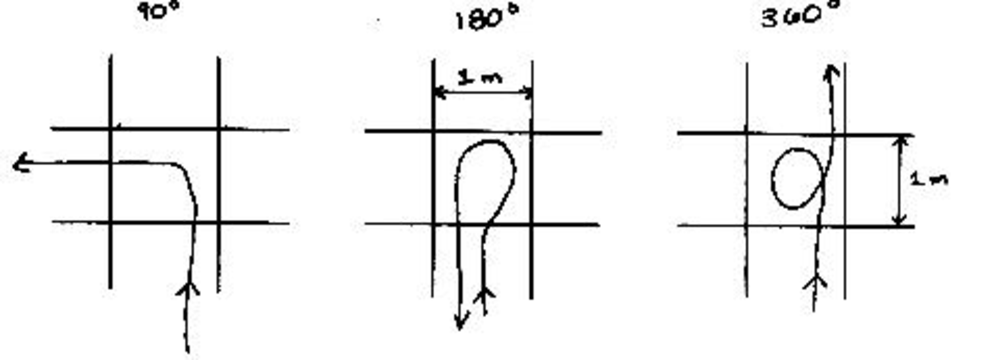
\includegraphics{degree_turns}
\end{center}
\vspace{-20pt}
\vspace{-10pt}
\end{figure}
 
\subsection{Level 3: 10 x 10 cm Obstacle}
The obstacle should be a rigid solid object.
The rider can ride or jump (forward or sideways) over the obstacle, using no external aids, as long as rider begins and ends the skill on the unicycle.

\subsection{Level 3: Hop 5 Times}
No external aids (bungee cords, toe clips, etc.), may be used for hopping.
The rider cannot travel more than 1 meter sideways while performing the skill.
The rider cannot rotate more than 180 degrees during the skill.

\subsection{Level 4/5: Idle 25 Times}
A rider cannot travel more than 1 meter sideways during the skill.
The rider cannot rotate more than 180 degrees during the skill.

\subsection{Level 5: Hop-Twist 90 Degrees}
Rider can be hopping prior to the execution of the skill.
90 degree Hop-twist must be a minimum of 90 degrees and a maximum of 135 degrees.

\subsection{Level 5/6: Seat on Side}
Seat and/or arm and hand can touch the body during this skill.
Seat on side to the right and left may be performed with the seat remaining on the same side for both.

\subsection{Level 6: Back turn/Front turn}
An adequate back turn/front turn is a continuous, linear flow of motion by the body while the wheel changes direction.
The motion should be fluid, and not like a turn, stop and turn, and the proper path looks like a cusp.
Front turns and back turns must be performed within two lines 30 cm apart.
This picture is a back turn.
For a front turn reverse the riding direction.

\begin{figure}[h]
\begin{center}
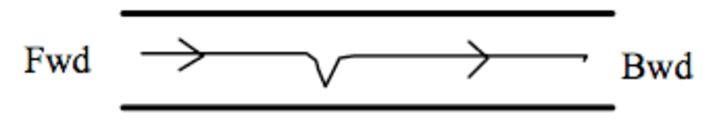
\includegraphics{fwd_bwd}
\end{center}
\vspace{-20pt}
\vspace{-10pt}
\end{figure}

\subsection{Level 6/7/8: Spins}
Spins must be performed within a 1 meter circle around a fixed point---no wandering spins.
Rider must perform 5 full rotations, but may need more than 5 full pedal rotations to complete these five spin rotations; no pirouettes are allowed.

\subsection{Level 7/8/9/10: Wheel Walk One-Footed}
This skill must be executed the full distance with the same foot always in control.
This skill may be performed with the non-pushing foot on the frame or extended.
A rider may not glide more than 1/2 revolution of the wheel during walk the wheel one-footed skills.

\subsection{Level 7: 180 Degree Hop-Twists}
Rider may be hopping prior to the execution of the skill.
180-degree hop-twist must be a minimum of 180 degrees and a maximum of 225 degrees.

\subsection{Level 8: Glide for 10 meters}
Gliding must be done on a level surface (not a slope).
The rider may not push the wheel during a glide (except for before and after the 10 meters of gliding for transitions).
During a glide there must be no contact with the pedals (except for before and after the 10 meters of gliding for transitions).
Gliding may be performed with the second foot on or off the frame.
During gliding, the rider is not allowed to coast (except for before and after the 10 meters of gliding for transitions).

\subsection{Level 8: Hand Wheel Walk}
Rider may be sitting on the seat \textbf{or} with the stomach on the seat.
However, the rider's feet may not touch the wheel, pedals, or the ground.

\subsection{Level 8/9: Pirouettes}
Pirouettes are three full 360-degree rotations and they must be performed with rider and unicycle rotating on a vertical axis.
There should be no pedal movement (forwards or backwards) during the pirouette.
When testing for pirouettes in Level 8 and 9, two testers must watch the pirouettes and come to a mutual agreement.
A rider must ride at least one revolution forwards before performing the forward pirouette.
A rider must ride at least one revolution backwards before performing the backwards pirouette.

\subsection{Level 9: Drag Seat in Front/Back}
When picking up drag seat in front/back, a rider may use either his/her hands or feet.

\subsection{Level 9: Seat in Front One-Footed for 10 Meters}
The rider shall have no contact with the seat other than the hand or hands holding the seat.
The hand(s) holding the seat as well as the corresponding arm(s) shall be extended away from the rider's body and shall not touch any part of the rider's body.

\subsection{Level 10: 180 Unispin}
The unicycle or the body of the rider must turn 180 degrees in a 180-unispin.
This skill may begin with hopping (seat out in front, or otherwise).
The rider must land the jump with both feet on pedals and the skill may end with the seat in
front or sitting on the seat.

\subsection{Level 10: Sideways Wheel Walk for 10 Meters}
Sideways wheel walk may be done with one or both feet.
Rider may not glide more than half revolution during the skill.

\subsection{Level 10: Coasting for 10 Meters}
During coasting you are not allowed to glide (except for before and after the 10 meters of coasting for transitions).
During coasting the rider may not come in contact with the wheel or pedals (except for before and after the 10 meters of coasting for transitions).
Must be performed on a level surface.
Coasting may be performed with either or both foot on the frame or extended.

\subsection{Level 10: Side Ride for 10 meters}
During side ride the rider may touch the seat with hands and body.
The rider's body from the waist down must be on one side of the unicycle.
The rider may choose how to hold the seat with either hands or forearms.
The controlling foot must be on the non-corresponding pedal (i.e. left foot on right pedal) and the other leg may not touch the unicycle.

\section{Mount Guidelines of the Skill Levels}

\subsection{General}
\begin{itemize}
\item For Level 3 and above, riders may not count their left and right foot mounts as different mounts.
\item The rider must declare his or her mount before being able to perform to the tester.
\item If a rider falls during the first attempt of the mount and/or ending, the rider must use that mount (and ending) for the second attempt.
\item The rider \textbf{must} end the mount by sitting on the seat with both feet on the pedals and riding a minimum of 3 revolutions.
For mounts that end in skills besides riding, the rider must do at least three revolutions, idles, or hops in the mounted position, and then end by sitting on the seat with both feet on the pedals and riding a minimum of three revolutions.
\item For Level 3 and above, riders must use the mounts clearly defined in section \ref{subsec:skill_mount-guidlines_mounts-for-level-3-and-above} of the IUF Rulebook.
No other mounts will be permitted by the IUF for reason of accurate and consistent level testing.
In addition, a rider may use a more difficult mount than the level he/she is testing for (i.e.
mount to hop on wheel may be used for Level 4).
\item For Level 7 and above, riders must mount to a skill defined in section \ref{subsec:skill_mount-guidlines_mounts-for-level-3-and-above} of the IUF Rulebook.
No other mountsor skills will be accepted.
\end{itemize}


\subsection{Mounts for Level 3 and above \label{subsec:skill_mount-guidlines_mounts-for-level-3-and-above}}
A testing rider is required to choose his/her mounts for Level 3 and above from the list below.
No other mount variations will be accepted by the IUF.
All selected mounts may be used once per test, but for Level 7 and above the ending skill may be repeated (i.e. wheel walk, 1 foot, seat in front, etc.).
Definitions for these mounts can be found in the Standard Skill portion, section \ref{sec:freestyle_std-skills-list}, of the IUF Rulebook.

\begin{multicols}{2}
\textbf{Level 3}
\begin{itemize}
\item Standard mount
\item Back mount
\item Rolling mount
\item Side mount
\item Reverse side mount
\item Jump mount
\end{itemize}

\textbf{Level 4}

Same as above, plus:
\begin{itemize}
\item Side jump mount
\item Spin mount 180 degrees
\item Floor mount
\end{itemize}
\columnbreak

\textbf{Level 5}

Same as above, plus:
\begin{itemize}
\item Kick up mount
\item Swing up mount to seat in front [Standard Skill 312a]
\end{itemize}

\textbf{Level 6}

Same as above, plus:
\begin{itemize}
\item Mount to wheel walk
\item Mount to hop on wheel
\end{itemize}
\end{multicols}

\textbf{Level 7 through 10}

All mounts must end in a skill as defined below:
\begin{multicols}{2}
\begin{itemize}
\item Standard mount to one foot / seat in front
\item Back mount to wheel walk / one foot idling
\item Side mount to seat on side / wheel walk
\item Rolling mount to one foot / gliding
\item Jump mount to seat in front / wheel walk
\item Floor mount to wheel walk / stand up wheel walk
\item Kick up mount to wheel walk
\item Swing up mount to seat in front [Standard Skill 312a]
\item Mount to hop on wheel
\item Mount to stand up wheel walk
\item Mount to drag seat in front
\item Mount to hand wheel walk
\item Mount to side hopping
\item Side jump mount to wheel walk / seat in back / 1ft idling
\item Mount to sideways wheel walk
\item Mount to side ride
\item Spin mount 360 degrees
\item Seat in front pick up mount [Standard Skill 311a]
\item Mount to seat in side stand-up wheel walk
\item Mount to crank idle
\end{itemize}
\end{multicols}

\newpage
\begingroup
 \small
\begin{multicols}{2}
\textbf{LEVEL 1}\\
mount unicycle unassisted\\
ride 50 meters\\
dismount gracefully with unicycle in front\\\\
\textbf{LEVEL 2}\\
mount with left foot\\
mount with right foot\\
ride 10 meters between two parallel lines 30 cm apart\\
ride a figure eight with circle diameters smaller than 3 meters\\
ride down a 15 cm vertical drop\\
make a 90 degree turn to the left inside a 1 meter square\\
make a 90 degree turn to the right inside a 1 meter square\\\\
\textbf{LEVEL 3}\\
demonstrate 3 types of mounts\\
ride a figure eight with circle diameters smaller than 1.5 meters\\
come to a stop, pedal half a revolution backward and continue forward\\
ride with the stomach on the seat for 10 meters\\
make a 180 degree turn to the left within a 1 meter square\\
make a 180 degree turn to the right within a 1 meter square\\
hop 5 times\\
ride or hop over a 10 x 10 cm.
obstacle\\\\
\textbf{LEVEL 4}\\
demonstrate 4 types of mounts\\
ride backward for 10 meters\\
ride one footed for 10 meters\\
idle with left foot down 25 times\\
idle with right foot down 25 times\\
ride with seat out in front (against body) for 10 meters\\
ride with the seat out in back (against body) for 10 meters\\
make a 360 degree turn to the left inside a 1 meter square\\
make a 360 degree turn to the right inside a 1 meter square\\
\columnbreak

\textbf{LEVEL 5}\\
demonstrate 5 types of mounts ride backward in a circle\\
ride one footed in a figure eight\\
idle one footed with the left foot 25 times\\
idle one footed with the right foot 25 times\\
ride with seat out in front (against body) in a circle\\
ride with the seat out in back (against body) in a circle\\
ride with the seat on the side (against body) in a circle\\
hop-twist 90 degrees to the left\\
hop-twist 90 degrees to the right\\
walk the wheel for 10 meters \\
\\
\textbf{LEVEL 6}\\
demonstrate 6 types of mounts\\
ride backward in a figure eight\\
ride with the seat out in front (against body) in a figure eight\\
ride with the seat out in back (against body) in a figure eight\\
ride backward with the seat out in front (against body) for 10 meters\\
hop standing on wheel 5 times\\
ride with the seat on the side (against body) in a circle to the left\\
ride with the seat on the side (against body) in a circle to the right\\
ride one footed with the left foot for 10 meters\\
ride one footed with the right foot for 10 meters\\
back turn\\
front turn\\
spin \\
\newpage
\textbf{LEVEL 7}\\
demonstrate 7 types of mounts\\
ride backward with the seat out in front (against body) in a circle\\
ride one footed with the left foot in a circle\\
ride one footed with the right foot in a circle\\
walk the wheel in a circle\\
walk the wheel one footed for 10 meters\\
hop-twist 180 degrees to the left\\
hop-twist 180 degrees to the right\\
ride backward with the seat out in back (against body) for 10 meters\\
spin to the left\\
spin to the right\\\\
\textbf{LEVEL 8}\\
demonstrate 8 types of mounts\\
ride one footed with the left foot in a figure eight\\
ride one footed with the right foot in a figure eight\\
walk the wheel in a figure eight\\
walk the wheel one footed in a circle\\
ride backward one footed for 10 meters\\
glide for 10 meters\\
hand wheel walk for 10 meters\\
pirouette\\
backward spin\\
\columnbreak

\textbf{LEVEL 9}\\
demonstrate 9 types of mounts\\
walk the wheel one footed in a figure eight\\
ride backward one footed in a circle\\
ride backward with the seat out in front (against body) in a figure eight\\
ride backward with the seat out in back (against body) in a circle\\
walk the wheel one footed with the left foot for 10 meters\\
walk the wheel one footed with the right foot for 10 meters\\
walk the wheel backward for 10 meters\\
drag seat in front for 10 meters\\
drag seat in back for 10 meters\\
ride backward one footed with the left foot for 10 meters\\
ride backward one footed with the right foot for 10 meters\\
one footed with the seat out in front for 10 meters\\
backward pirouette\\\\
\textbf{LEVEL 10}\\
demonstrate 10 types of mounts\\
ride backward with the seat out in back (against body) in a figure eight\\
ride backward one footed in a figure eight\\
walk the wheel one footed with the left foot in a circle\\
walk the wheel one footed with the right foot in a circle\\
walk the wheel backward in a circle\\
180 uni spin\\
sideways wheel walk for 10 meters\\
coast for 10 meters\\
side ride for 10 meters\\
walk the wheel one footed backward for 10 meters\\
\end{multicols}
\endgroup



\end{document} % Have to typset (ctrl-t) twice (or three times) to get everything to work
